%!TEX root = main.tex

\documentclass[
  % draft,
  % final,
  a4paper,
  % 11pt,
  % twoside,
  % BCOR=1cm,
  twoside=semi,
  % oneside,
  % parskip=half,
  toc=bibliography,
  toc=listof,
  chapterprefix=true,
  version=last,
  cleardoublepage=empty,
]{scrbook}

%!TEX root = main.tex

%%% Grundlegendes

% Verwende etex als zugrundeliegende Implementierung (-> mehr Speicher für Tex!)
\usepackage{etex}
% Encoding
\usepackage[utf8]{inputenc}


%%% Schriften, Lokalisierung und Typographie

% T1 Schriftsystem verwenden
\usepackage[T1]{fontenc}
% LModern als Standard-Schrift
\usepackage{lmodern}
% Typographische Kleinigkeiten
\usepackage{microtype}
% Fraktur-Schriftsatz
\usepackage{eufrak}

%% Lokalisierung

% Deutsche Silbentrennung
\usepackage[english,ngerman]{babel}
% Deutsche Anführungszeichen
\usepackage[babel,german=quotes]{csquotes}

%% Weitere Schriften vordefinieren

\newcommand{\altfont}{\fontfamily{qpl}}
% \newcommand{\altsffont}{\fontfamily{phv}}
\newcommand{\altsffont}{\fontfamily{pfr}\fontseries{l}}

% Zeilenabstand anpassen (MUST NOT USE!)
% \usepackage{setspace}
% \setstretch{1.1}

% Textsatzbereich nach unten vergrößern
% TODO: richtig konfigurieren
% \usepackage[a4paper,twoside,bottom=4cm]{geometry}

%%% Graphiken und Farben

% Graphiken und Farben
\usepackage{xcolor}
\usepackage{graphicx}

% Vordefinierte Farben laden
\definecolor{jgu_rot}{RGB}{193,0,42}
\definecolor{jgu_hellgrau}{RGB}{172,172,172}
\definecolor{jgu_dunkelgrau}{RGB}{99,99,99}
\definecolor{matlab_blau}{rgb}{0.00000,0.44700,0.74100}
\definecolor{matlab_orange}{rgb}{0.85000,0.32500,0.09800}


% Caption anpassen und Subfigures erlauben
\usepackage[style=base,font+=small,labelfont+=bf,margin=1em]{caption}
\usepackage{subcaption}

% Tikz ist kein Zeichenprogramm!
\usepackage{tikz}
\usepackage{pgfplots}
\pgfplotsset{compat=1.12}
\usetikzlibrary{patterns}

% Standalone-Paket, damit die Tikz Bilder extern auch funktionieren
\usepackage{standalone}


%%% Bibliographie

\usepackage[%
    backend=biber,
    style=alphabetic,
    backref=true,
    firstinits=true
]{biblatex}

% Fix für doi2bib generierte Bibliography-Einträge
\newcommand\mathplus{+}


%%% Grundlegende Mathematik-Pakete

% Standardpackages
\usepackage{amsmath}
\usepackage{amssymb}
\usepackage{stmaryrd}
\usepackage{mathtools}

% "Bessere" Theorem-Umgebungen
\usepackage[
    amsmath,
    thmmarks,
    hyperref,
]{ntheorem}


%%% Hyperref

\usepackage[
	colorlinks=true,
	linkcolor=jgu_rot,          % color of internal links (change box color with linkbordercolor)
	citecolor=jgu_rot,        % color of links to bibliography
	filecolor=jgu_rot,      % color of file links
	urlcolor=jgu_rot,
    hypertexnames=false
]{hyperref}


%%% Clevere Referenzen

\usepackage[german,noabbrev,nameinlink,capitalise]{cleveref}
\crefname{equation}{}{}

% Nummern nur für referenzierte Gleichungen
\usepackage{autonum}


%%% Layout und Stil

% Fancyhdr-Ersatz für scrbook
\usepackage[
    automark,
    % headsepline,
    draft=false
]{scrlayer-scrpage}

% Inhaltsverzeichnis anpassen (Schriften angleichen!)
\usepackage{tocstyle}
\usetocstyle{KOMAlike}

%% Chapter-Style und mehr

% Alle Überschriften in TeX Gyre Pagella
\addtokomafont{disposition}{\normalfont\altfont\selectfont}
% Alle Überschriften in Dunkelgrau
% \addtokomafont{disposition}{\color{jgu_dunkelgrau}}

% Einzelne Optionen bei Bedarf
% \addtokomafont{chapter}{\normalfont\altfont\selectfont}
% \addtokomafont{chapter}{\color{black}}
% \addtokomafont{section}{\normalfont\altfont\selectfont}
% \addtokomafont{subsection}{\normalfont\altfont\selectfont}
% \addtokomafont{subsubsection}{\normalfont\altfont\selectfont}
% \addtokomafont{minisec}{\normalfont\altfont\selectfont}
% \addtokomafont{paragraph}{\normalfont\altfont\selectfont}
\addtokomafont{paragraph}{\bfseries}

% Kopfzeile anpassen
\addtokomafont{pageheadfoot}{\color{jgu_dunkelgrau}\normalfont\altfont\selectfont}
% Seitenzahl anpassen
\addtokomafont{pagenumber}{\color{jgu_dunkelgrau}\normalfont\altfont\selectfont}

% Zitatblock für Kapitelanfang
\renewcommand*\dictumwidth{.95\linewidth}
\renewcommand*\dictumrule{}
\renewcommand*\dictumauthorformat[1]{--- #1}
\addtokomafont{dictumtext}{\color{jgu_dunkelgrau}\normalfont\altsffont\fontsize{9}{12}\selectfont\itshape}
\addtokomafont{dictumauthor}{\color{jgu_dunkelgrau}\normalfont\altsffont\fontsize{8}{12}\selectfont}

% Kapitel-Stil
\renewcommand*{\chapterheadstartvskip}{\vspace*{3\baselineskip}}
\renewcommand*{\chapterheadendvskip}{\vspace*{2\baselineskip}}
\renewcommand*{\chapterformat}{%
				\raggedright
				\color{jgu_rot}
                \altfont\fontsize{60}{30}\selectfont\thechapter
                \fontsize{20}{30}\scshape\selectfont\enskip\chapappifchapterprefix
                }
\renewcommand*{\raggedchapter}{\raggedleft}

% Inhaltsverzeichnis
% \addtokomafont{sectionentrypagenumber}{\color{black}}
\addtokomafont{chapterentrypagenumber}{\color{black}\rmfamily}
\addtokomafont{chapterentry}{\rmfamily\bfseries}


%%% Verzeichnisse

% Akronymverzeichnis
\usepackage{acro}
\acsetup{
    page-ref=paren,
    pages=first,
    page-name={siehe S.\@\,},
}

% Symbolverzeichnis
\usepackage[german,intoc]{nomencl}
\setlength{\nomitemsep}{-\parsep}
\makenomenclature


% ntheorem-Umgebungen laden
%%
%% This is file `ntheorem.std',
%% generated with the docstrip utility.
%%
%% The original source files were:
%%
%% ntheorem.dtx  (with options: `standard')
%%
%% IMPORTANT NOTICE:
%%
%% For the copyright see the source file.
%%
%% Any modified versions of this file must be renamed
%% with new filenames distinct from ntheorem.std.
%%
%% For distribution of the original source see the terms
%% for copying and modification in the file ntheorem.dtx.
%%
%% This generated file may be distributed as long as the
%% original source files, as listed above, are part of the
%% same distribution. (The sources need not necessarily be
%% in the same archive or directory.)
\def\filedate{2011/08/15}
\def\docdate{2011/08/15}
\def\fileversion{1.33}
\def\basename{ntheorem}
%% This file may be distributed and/or modified under the
%% conditions of the LaTeX Project Public License, either version 1.2
%% of this license or (at your option) any later version.
%% The latest version of this license is in
%%    http://www.latex-project.org/lppl.txt
%% and version 1.2 or later is part of all distributions of LaTeX
%% version 1999/12/01 or later.
%% \CharacterTable
%%  {Upper-case    \A\B\C\D\E\F\G\H\I\J\K\L\M\N\O\P\Q\R\S\T\U\V\W\X\Y\Z
%%   Lower-case    \a\b\c\d\e\f\g\h\i\j\k\l\m\n\o\p\q\r\s\t\u\v\w\x\y\z
%%   Digits        \0\1\2\3\4\5\6\7\8\9
%%   Exclamation   \!     Double quote  \"     Hash (number) \#
%%   Dollar        \$     Percent       \%     Ampersand     \&
%%   Acute accent  \'     Left paren    \(     Right paren   \)
%%   Asterisk      \*     Plus          \+     Comma         \,
%%   Minus         \-     Point         \.     Solidus       \/
%%   Colon         \:     Semicolon     \;     Less than     \<
%%   Equals        \=     Greater than  \>     Question mark \?
%%   Commercial at \@     Left bracket  \[     Backslash     \\
%%   Right bracket \]     Circumflex    \^     Underscore    \_
%%   Grave accent  \`     Left brace    \{     Vertical bar  \|
%%   Right brace   \}     Tilde         \~}

\theoremnumbering{arabic}
\theoremstyle{plain}
\RequirePackage{latexsym}
% \theoremsymbol{\ensuremath{_\Box}}
\theorembodyfont{\itshape}
\theoremheaderfont{\normalfont\bfseries}
\theoremseparator{}
\newtheorem{Theorem}{Theorem}[chapter]
\newtheorem{theorem}[Theorem]{Theorem}
\newtheorem{Satz}[Theorem]{Satz}
\newtheorem{satz}[Theorem]{Satz}
\newtheorem{Proposition}[Theorem]{Proposition}
\newtheorem{proposition}[Theorem]{Proposition}
\newtheorem{Lemma}[Theorem]{Lemma}
\newtheorem{lemma}[Theorem]{Lemma}
\newtheorem{Korollar}[Theorem]{Korollar}
\newtheorem{korollar}[Theorem]{Korollar}
\newtheorem{Corollary}[Theorem]{Corollary}
\newtheorem{corollary}[Theorem]{Corollary}

\theorembodyfont{\upshape}
\newtheorem{Example}[Theorem]{Example}
\newtheorem{example}[Theorem]{Example}
\newtheorem{Beispiel}[Theorem]{Beispiel}
\newtheorem{beispiel}[Theorem]{Beispiel}
\newtheorem{Bemerkung}[Theorem]{Bemerkung}
\newtheorem{bemerkung}[Theorem]{Bemerkung}
\newtheorem{Anmerkung}[Theorem]{Anmerkung}
\newtheorem{anmerkung}[Theorem]{Anmerkung}
\newtheorem{Remark}[Theorem]{Remark}
\newtheorem{remark}[Theorem]{Remark}
\newtheorem{Definition}[Theorem]{Definition}
\newtheorem{definition}[Theorem]{Definition}
\newtheorem{Annahme}[Theorem]{Annahme}
\newtheorem{annahme}[Theorem]{Annahme}

\theoremstyle{nonumberplain}
\theoremheaderfont{\scshape}
\theorembodyfont{\normalfont}
\theoremseparator{.}
\theoremsymbol{\ensuremath{_\square}}
\RequirePackage{amssymb}
\newtheorem{Proof}{Proof}
\newtheorem{proof}{Proof}
\newtheorem{Beweis}{Beweis}
\newtheorem{beweis}{Beweis}
\qedsymbol{\ensuremath{_\square}}

\theoremstyle{nonumberplain}
\theoremheaderfont{\normalfont\bfseries}
\theoremseparator{}
\theorembodyfont{\normalfont}
\theoremsymbol{}
\RequirePackage{amssymb}
\newtheorem{Problem}{Problem}
\newtheorem{problem}{Problem}
\qedsymbol{}

\theoremclass{LaTeX}
\endinput
%%
%% End of file `ntheorem.std'.



%%% Alles andere

% Querformatseiten
\usepackage{pdflscape}

% Enumerates anpassen
\usepackage{enumitem}
% Numerierte Umgebung für Theoreme definieren
\newlist{thmenumerate}{enumerate}{1}
\setlist[thmenumerate]{label={\upshape(\roman*)}, align=left, widest=iii, leftmargin=*}
\crefname{thmenumeratei}{}{}

% Konturen um Text zeichnen
\usepackage[outline]{contour}
\contourlength{0.09em}

% Gepunktete Linien
\usepackage{dashrule}


%%% "Debugging"

% Labels am Seitenrand anzeigen
\usepackage[
    inline,
    final
]{showlabels}

% todos
\usepackage[%
    german,
    colorinlistoftodos,
    % disable
]{todonotes}

% Todos vordefinieren
\newcommand{\mdo}[1]{\todo[color=yellow!50]{#1}}
\newcommand{\mfix}[1]{\todo[color=red!50]{#1}}
\newcommand{\mwarn}[1]{\todo[color=blue!50]{#1}}

% Blindtext
\usepackage{blindtext}
\blindmathtrue{}

% etoolbox?
\usepackage{etoolbox}

% \usepackage{showframe}



%!TEX root = main.tex

% griechisches Alphabet anpassen
\renewcommand{\epsilon}{\varepsilon}
\renewcommand{\theta}{\vartheta}


%%% Operatoren und anderes mathematisches Geplänkel

% Beträge und Normen
\DeclarePairedDelimiter{\abs}{\lvert}{\rvert}
\DeclarePairedDelimiter{\norm}{\lVert}{\rVert}

% Gauß-Klammern
\DeclarePairedDelimiter{\ceil}{\lceil}{\rceil}
\DeclarePairedDelimiter{\floor}{\lfloor}{\rfloor}

% Skalarprodukte und Duale Paarungen
\newcommand{\skprod}[2]{\left\langle#1,#2\right\rangle}
\newcommand{\Skp}[3]{\left\langle#1,#2\right\rangle_{#3}}
\newcommand{\skp}[3]{\langle#1,#2\rangle_{#3}}
\newcommand{\Dual}[2]{\left(#1,#2\right)}
\newcommand{\dual}[2]{(#1,#2)}

% Inneres und Äußeres
\newcommand{\Int}[1]{#1^\circ}
\newcommand{\Ext}[1]{\overline{#1}}

% Diverse Operatoren
\DeclareMathOperator{\spn}{span}
\DeclareMathOperator{\ee}{e}
\DeclareMathOperator{\ii}{i}
\newcommand{\Transp}{^{\mathrm{T}}}
\newcommand{\Stern}{^{*}}
\newcommand{\grad}{\nabla}
\DeclareMathOperator{\divergenz}{div}
\newcommand{\hesse}{\nabla^2}

% Einschränkung einer Funktion
\newcommand\restr[2]{\ensuremath{\left.#1\right|_{#2}}}

% Ordentlicher Befehl um Mengen zu setzen
\providecommand\given{} % so it exists
\newcommand\SetSymbol[1][]{
   \nonscript\,#1\vert\nonscript\,\mathopen{}\allowbreak}
\DeclarePairedDelimiterX\Set[1]{\lbrace}{\rbrace}{ \renewcommand\given{\SetSymbol[\delimsize]} #1 }

% Vektoren und Matrizen anders setzen
\renewcommand{\vec}[1]{\mathbf{#1}}
\newcommand{\mat}[1]{\mathbf{#1}}

% Differential-d für Integral ordentlich setzen
\newcommand*\diff{\mathop{}\!\mathrm{d}}
\newcommand*\Diff[1]{\mathop{}\!\mathrm{d^#1}}

% wesentliches Supremum
\DeclareMathOperator*{\esssup}{ess\,sup}
\newcommand\blank{{\mkern2mu\cdot\mkern2mu}}

% "Definition-Gleich"
% FIXME: deprecated
\newcommand\deq{\coloneqq}

% dichte Einbettung
% FIXME: zu hoch für Fließtext!
\newcommand\denseinclusion{\stackrel{d}{\hookrightarrow}}

% Schrift einfach anpassen
\newcommand{\changefont}[3]{
\fontfamily{#1} \fontseries{#2} \fontshape{#3} \selectfont}


%%% Textbausteine

\newcommand{\fa}{\text{für alle}~}

% um fremde Begriffe einheitlich mit Übersetzung zu setzen
\newcommand\foreign[2]{#1 \textit{#2}}

%!TEX root = main.tex

\newcommand{\titel}{- in Arbeit - Parabolische partielle Differentialgleichungen und Reduzierte-Basis-Methoden}
\newcommand{\art}{Masterarbeit}
\newcommand{\autor}{Alexej Disterhoft}
\newcommand{\fach}{Mathematik}
\newcommand{\matrikelnr}{2669611}
\newcommand{\erstgutachter}{JProf. Dr. Thorsten Raasch}
\newcommand{\zweitgutachter}{???}
\newcommand{\monat}{Irgendwann}
\newcommand{\jahr}{2015}
\newcommand{\ort}{Mainz}
\newcommand{\logo}{figures/misc/logo_gross.eps}

\hypersetup{pdfinfo={
  Title=\titel,
  Author=\autor}
}

%!TEX root = main.tex

\DeclareAcronym{scft}{
	short            = SCFT,
	long             = selbstkonsistente Feldtheorie,
	long-plural-form = selbstkonsistenten Feldtheorie,
	short-plural     = {},
	foreign          = \foreign{engl.}{self-consistent field theory}
}

\DeclareAcronym{rbm}{
	short = RBM,
	long  = Reduzierte-Basis-Methode
}

\DeclareAcronym{fem}{
	short = FEM,
	long = Finite-Elemente-Methode
}

\DeclareAcronym{bnb}{
	short = BNB,
	long = Banach-Ne{\v c}as-Babu{\v s}ka-Theorem
}

\DeclareAcronym{SCM}{
	short = SCM,
	long = Successive Constraint Method
}


\usepackage{dirtree}

\addbibresource{literature.bib}

\begin{document}
    %%% Frontmatter-Teil
    \frontmatter{}

    % Deckblack / Titelseite
    %!TEX root = ../main.tex

\thispagestyle{plain}
\begin{titlepage}
\begin{center}
% $\;$\\[2em]
\includegraphics[scale=1.5,clip,trim=0em 2em 0em 2.8em]{\logo}\\[3em]
%
% {\fontfamily{qpl}\selectfont{\LARGE{\textbf{\titel}}\par}}
{\fontfamily{qpl}\selectfont{\LARGE{\textbf{Numerische Behandlung von \\Self-Consistent Field Theory-Modellen\\ mittels Reduzierter-Basis-Methoden}}\par}}
\normalsize$\;$\\[1em]
{\large{\textbf{\art}}}\\[1em]
{\normalsize
am Institut für Mathematik,\\
Fachbereich Physik, Mathematik und Informatik\\
der Johannes Gutenberg-Universität\\
in Mainz
}\\[6em]
%
{\large{\textbf{\autor}}}\\[0.4em]
{\normalsize{geboren in Leonidowka}}\\[4em]
%
\begin{tabular}{p{3cm}p{7cm}}\\
Erstgutachter:  & \quad \erstgutachter\\[1.2ex]
Zweitgutachter: & \quad \zweitgutachter\\[3ex]
\end{tabular}

{\ort,~\today}
% {\ort,~\monat~\jahr}
%
\end{center}
\end{titlepage}


    % Danksagung
    % %!TEX root = ../main.tex

\thispagestyle{plain}
\begin{titlepage}
\dictum[Andy Weir, \textit{The Martian}]{\enquote{I guess you could call it a \enquote{failure}, but I prefer the term \enquote{learning
experience}.}}
\vfill{}
\begin{flushright}
% \emph{Für meine Eltern.}
\end{flushright}
\end{titlepage}


    % Abstrakt
    % %!TEX root = ../main.tex

\chapter{Zusammenfassung} % (fold)
\label{cha:Zusammenfassung}

\blindtext

% chapter Zusammenfassung (end)


    % Inhaltsverzeichnis
    \tableofcontents

    % TODO-Liste
    % \listoftodos

    %%% Hauptteil
    \mainmatter{}

    % Kapitel einbinden
    %!TEX root = ../main.tex

\chapter{Einleitung} % (fold)
\label{chapter:einleitung}

Der Begriff \emph{Polymer} bezeichnet einen aus Makromolekülen bestehenden Stoff.
Diese Makromoleküle setzen sich wiederum aus vielen kleineren, sich wiederholenden Molekülen, in diesem Zusammenhang Monomere genannt, zusammen.
Besteht ein Polymer aus nur einer Monomer-Gattung, dann spricht man von einem Homopolymer, sonst von einem Heteropolymer oder auch Copolymer.
Obwohl Polymere in vielen verschiedenen Konfigurationen, beispielsweise ring- oder sternförmig, auftreten können, beschränken wir uns hier auf den Fall eines kettenförmigen Aufbaus.
Weiter interessieren wir uns hier nur für Copolymere, vor allem die sogenannten Blockcopolymere, welche aus mehreren Monomer-Gattungen, die homogene zusammenhängende Blöcke bilden, aufgebaut sind; siehe \cref{figure:polymerketten}.

\begin{figure}[tb]
    \centering
    \begin{subfigure}[b]{\textwidth}
        \centering
        \includestandalone[width=0.7\textwidth]{tikz/einleitung/fig1}
    \end{subfigure}
    \\[0.33em]
    \begin{subfigure}[b]{\textwidth}
        \centering
        \includestandalone[width=0.7\textwidth]{tikz/einleitung/fig2}
    \end{subfigure}
    \\[0.33em]
    \begin{subfigure}[b]{\textwidth}
        \centering
        \includestandalone[width=0.7\textwidth]{tikz/einleitung/fig3}
    \end{subfigure}
    \caption[Skizzenhafte Darstellung verschiedener Polymerarten]{%
        Skizzenhafte Darstellung verschiedener Polymerarten.
        Von oben nach unten: Homopolymer, ein AB-Diblockcopolymer und ein sogenanntes statistisches AB-Copolymer, bei dem die beiden Monomer-Arten zufällig verteilt sind.
    }
    \label{figure:polymerketten}
\end{figure}

Von besonderem Interesse ist nun das Verhalten von Polymerschmelzen (\foreign{engl.}{polymer melt}), das heißt, des flüssigen Aggregatzustands eines Polymers, sowie das Verhalten von Gemischen verschiedener polymerer Stoffe.
So neigen die Gemische vieler Paare von Homopolymeren zu makroskopischer Phasenseparation, wie man es beispielsweise auch von Öl und Essig kennt.
Eine ähnliche Tendenz zur Separation findet man auch bei Schmelzen von Blockcopolymeren, hierbei ist aber aufgrund der Verbindung zwischen den verschiedenen Monomer-Blöcken keine makroskopische Phasenseparation möglich, stattdessen kommt es zu einer periodischen mikroskopischen Separation, vergleiche \cref{figure:phasen}.

Da die experimentelle Bestimmung ohne Vorwissen über mögliche stabile Anordnungen nur wenig erfolgversprechend ist, wird ein theoretisches Fundament benötigt, auf Basis dessen Vorhersagen getroffen werden können, die vorzugsweise auch zu experimentell belegbaren Anordnungen führen.
Wir beschränken uns auf die Betrachtung von Diblockcopolymeren, das heißt, Blockcopolymeren, die aus zwei verschiedenen Monomer-Gattungen bestehen, da diese ein vergleichsweise einfaches System darstellen.

Als nützliches und relativ gut handhabbares theoretisches Modell hat sich die sogenannte \ac{scft} herausgestellt, die im Folgenden eingeführt und erläutert wird.

\begin{figure}[tb]
    \centering
    \begin{subfigure}[b]{0.15\textwidth}
        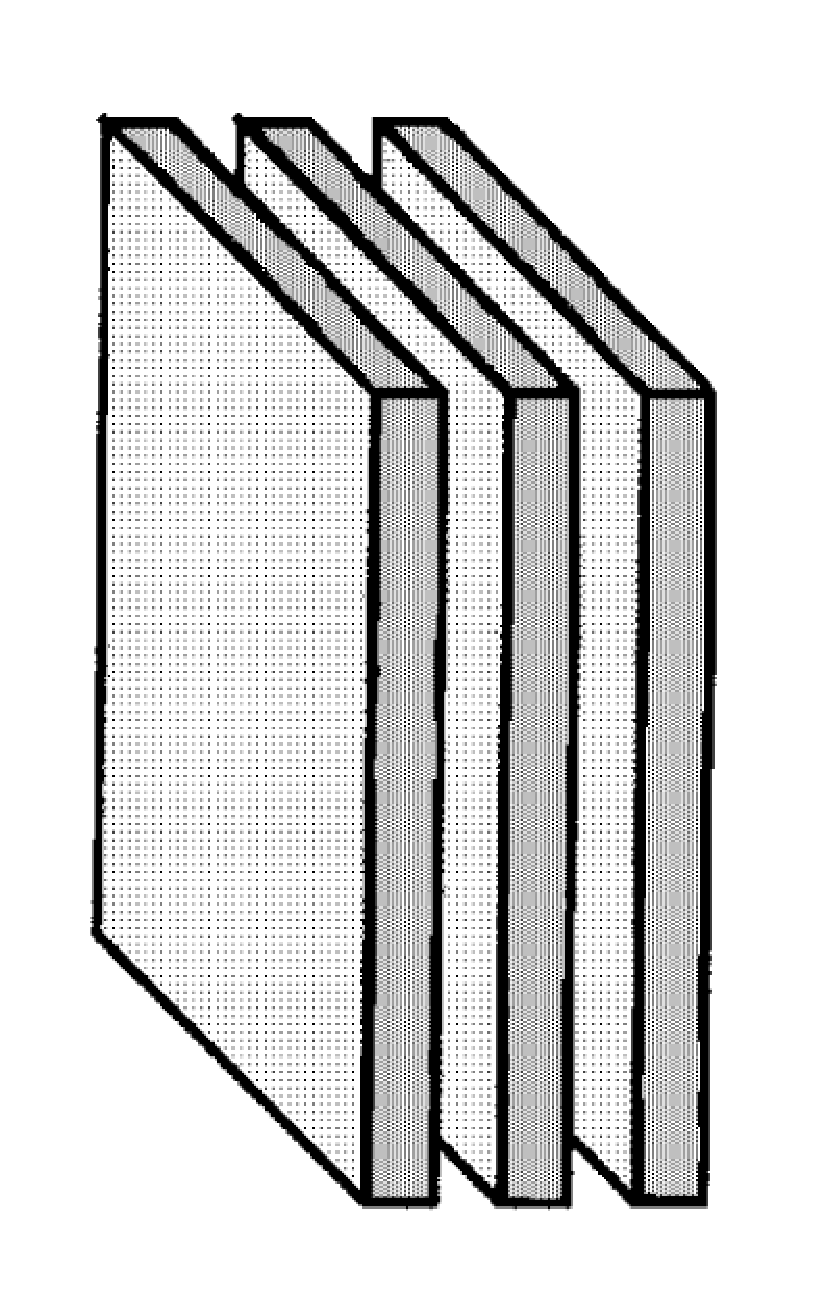
\includegraphics[width=\textwidth]{figures/einleitung/fig1}
    \end{subfigure}
    \begin{subfigure}[b]{0.15\textwidth}
        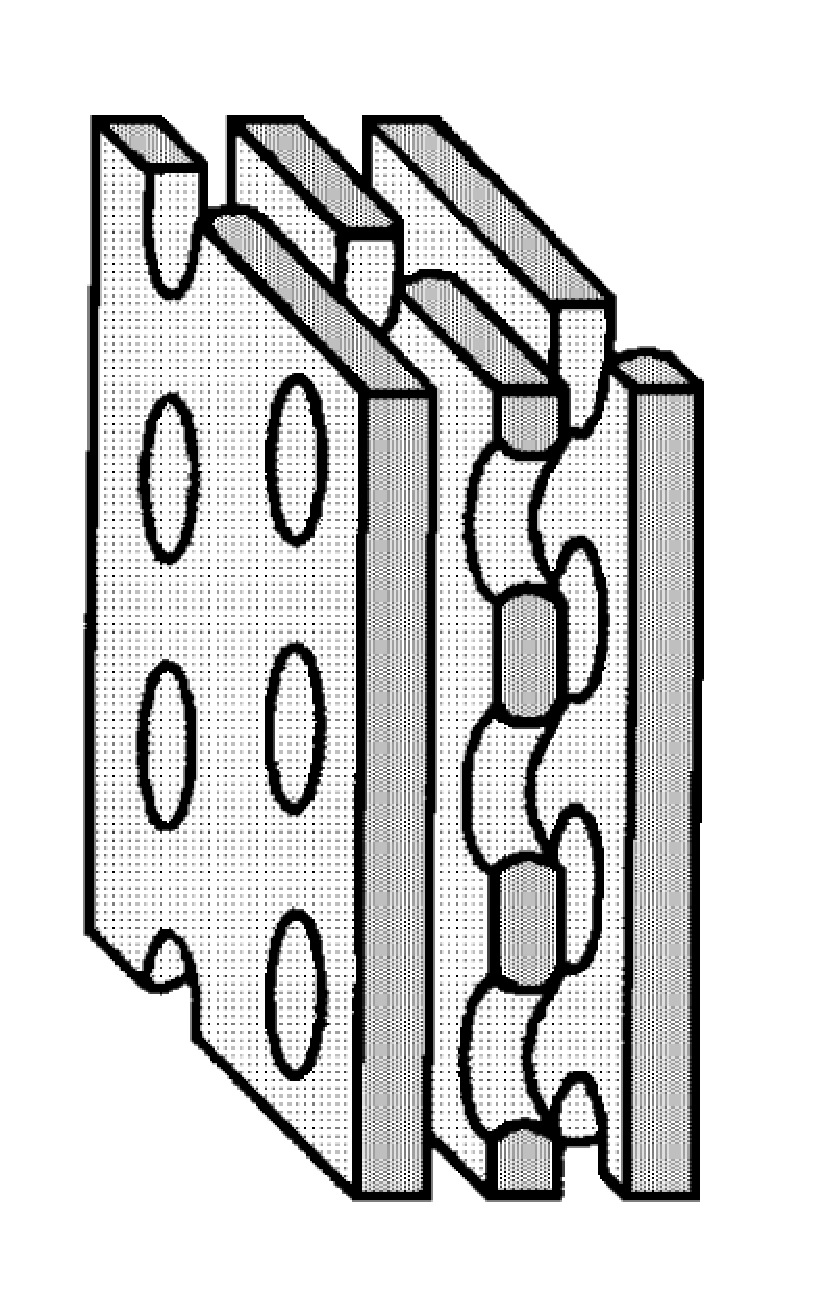
\includegraphics[width=\textwidth]{figures/einleitung/fig2}
    \end{subfigure}
    \begin{subfigure}[b]{0.15\textwidth}
        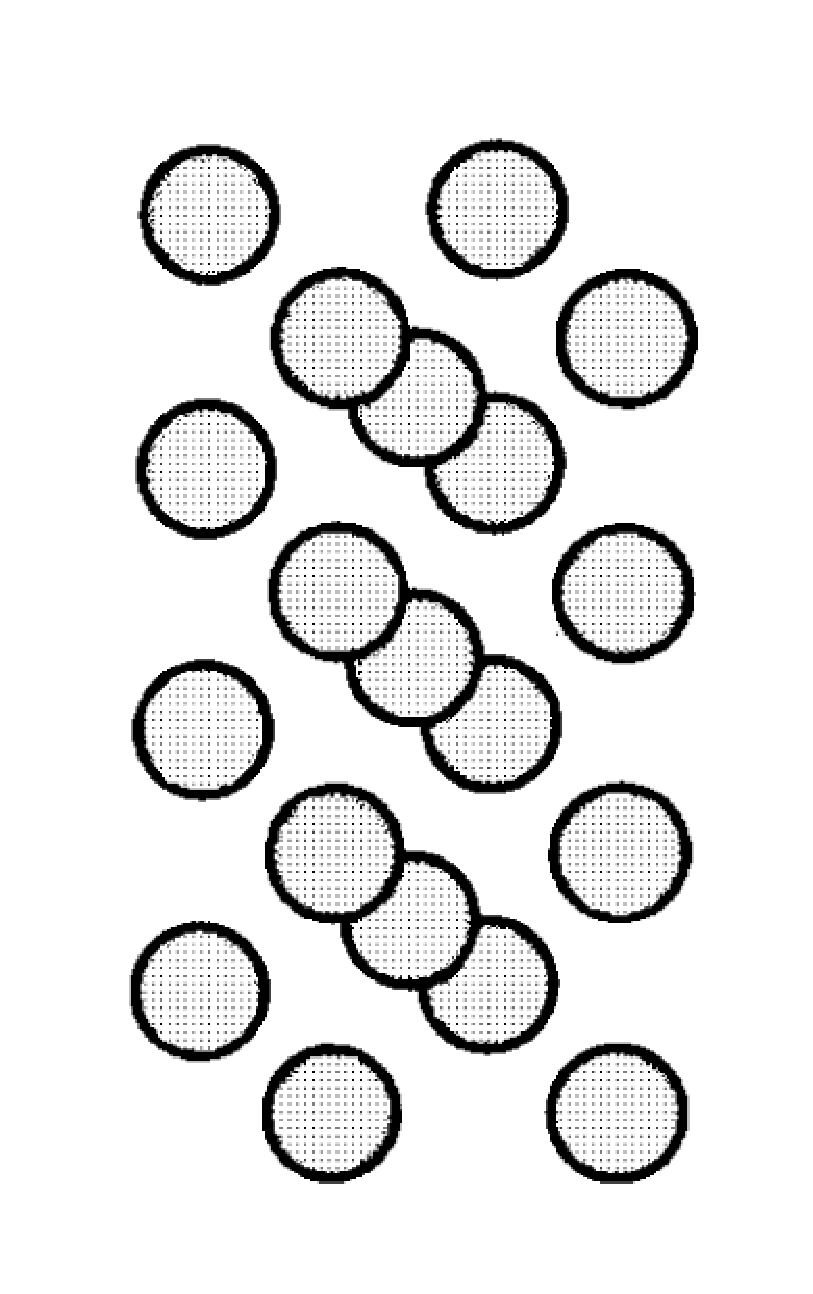
\includegraphics[width=\textwidth]{figures/einleitung/fig3}
    \end{subfigure}
    \begin{subfigure}[b]{0.15\textwidth}
        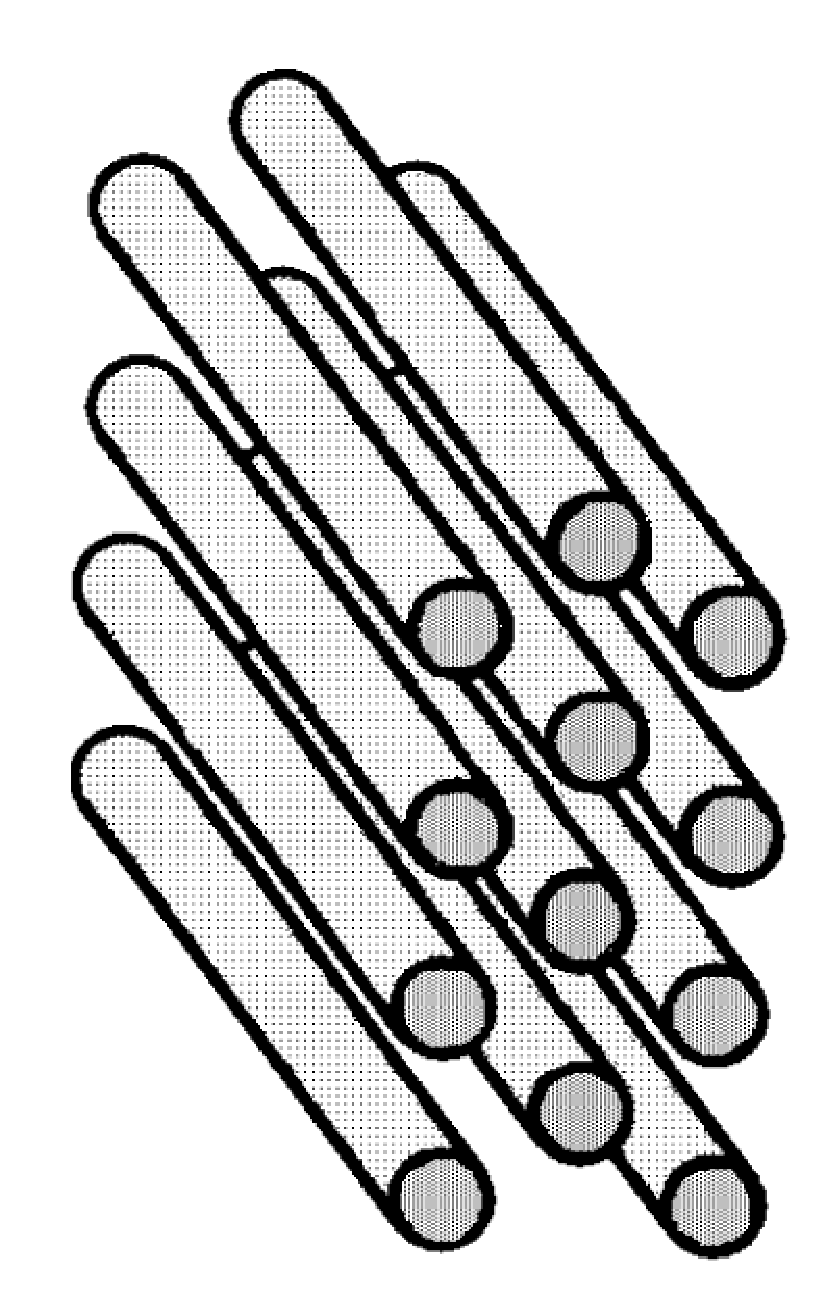
\includegraphics[width=\textwidth]{figures/einleitung/fig4}
    \end{subfigure}
    \begin{subfigure}[b]{0.15\textwidth}
        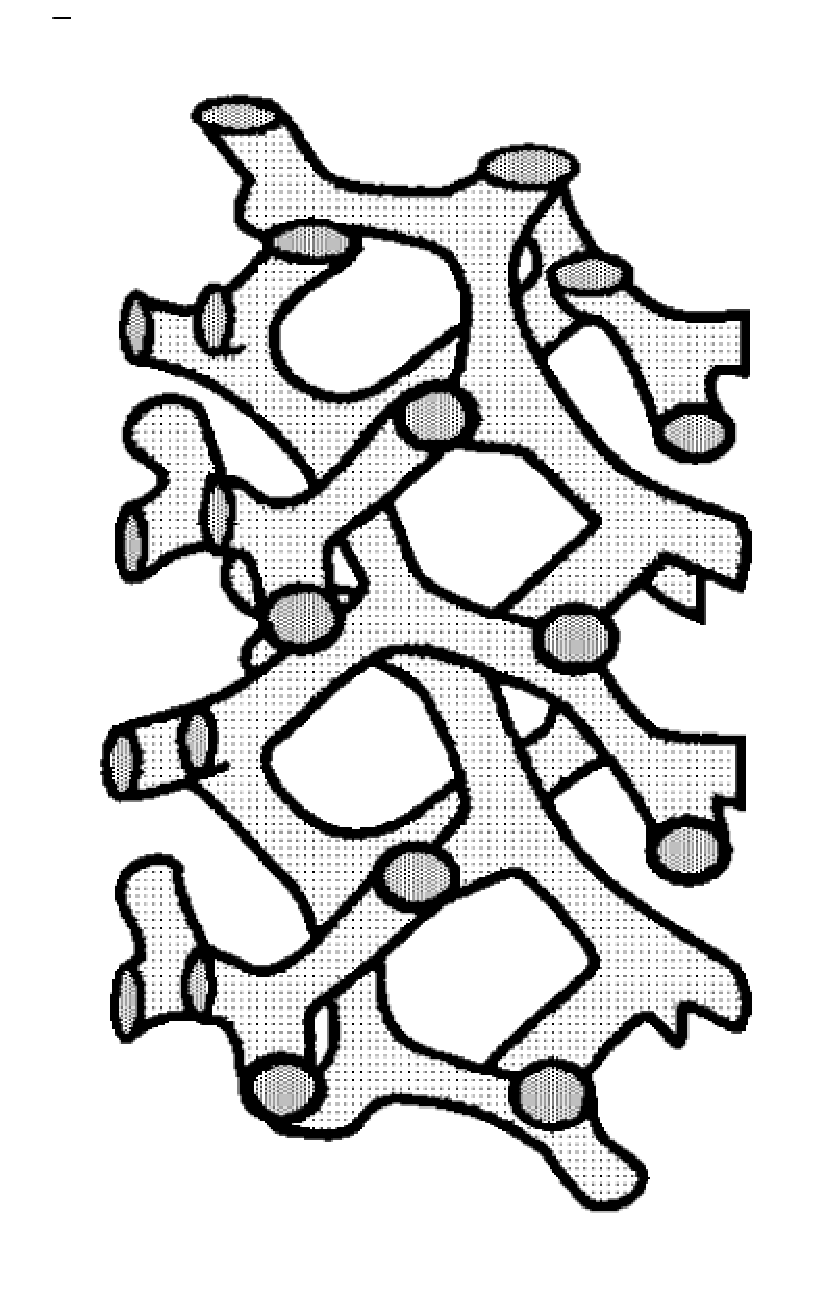
\includegraphics[width=\textwidth]{figures/einleitung/fig5}
    \end{subfigure}
    \caption[Verschiedene Phasen bei Diblockcopolymeren]{%
        Verschiedene Phasen bei Diblockcopolymeren, welche experimentell beobachtet wurden, wobei hierbei nur eine der beiden Monomer-Gattungen dargestellt wird.
        Diese heißen von links nach rechts: lamellar, perforiert-lamellar, sphärisch, zylindrisch, gyroid.
        Diese Abbildung wurde \cite[Figure 1.18]{Matsen:2006ud} entnommen.
    }
    \label{figure:phasen}
\end{figure}

\subsection*{Mathematische Modellierung} % (fold)

Als Grundlage für die \acl{scft} dient eine Modellierung der Polymere als frei bewegliche Ketten (\foreign{engl.}{ideal chain}).
Im Rahmen dieser Arbeit betrachten wir zwar nur die aus dem sogenannten stetigen Gaußschen Kettenmodell resultierende Theorie, erläutern aber zunächst ein diskretes Kettenmodell, welches eine Vorstufe des stetigen darstellt und die Idee dahinter verdeutlicht.
Eine deutlich ausführlichere und vor allem mathematisch begründete Einführung in diese Thematik findet man bei \textcites[Chapter 2]{Fredrickson:2006th}{rubinstein2003polymer}.

Im Folgenden betrachten wir eine nicht näher spezifizierte Volumenzelle und geben mit dem Vektor $\vec{r}$ eine Position in diesem Volumen an.

Das diskrete Modell stellt die Polymerkette als eine diskrete Kette von Partikeln dar, derart, dass aneinanderhängende Monomere ähnlich einem Scharnier frei beweglich sind.
Dabei werden Wechselwirkung zwischen benachbarten Monomeren berücksichtigt, während auf der Kette weit auseinanderliegende Partikel aber ignoriert werden.
Diese Wechselwirkungen können in \cref{figure:kettenmodelle} beispielsweise als Einschränkung des Winkels $\vartheta_9$ durch die gegenseitige Beeinflussung der Partikel $8, 9$ und $10$ auftreten.

Das stetige Gaußsche Kettenmodell, welches man unter anderem auch als stetigen Grenzfall des beschriebenen diskreten Modells erhält, hat sich als besonders nützlich erwiesen, sowohl bei analytischen als auch numerischen Betrachtungen.
Dabei wird die Polymerkette als stetige, linear elastische Faser aufgefasst und durch eine Kurve $\vec{r}(s)$ parametrisiert, wobei $s \in [0, 1]$ eine entlang der normalisierten Kontur der Kette verlaufende Variable ist.

\begin{figure}[tb]
    \centering
        \includestandalone[width=0.6\textwidth]{tikz/einleitung/chains}
    \caption[%
        Polymerkette in diskretem und Gaußschen Kettenmodell
    ]{%
        Schematische Darstellung einer Polymerkette im diskreten Kettenmodell (links) und im stetigen Gaußschen Kettenmodell (rechts).
        Abbildung reproduziert nach \cite[Figure 2.1 und 2.5]{Fredrickson:2006th}.
    }
    \label{figure:kettenmodelle}
\end{figure}

Sowohl das diskrete als auch das stetige Kettenmodell haben einen starken Bezug zur Stochastik, da sie sich auch als Random Walks beziehungsweise stochastische Prozesse auffassen lassen.
Dies stellt einen umfangreichen \enquote{Werkzeugkasten} zur Untersuchung dieser zur Verfügung.
Da die benötigten stochastischen Ausführungen und Herleitungen für diese Arbeit jedoch nebensächlich sind, belassen wir es bei diesen informalen Beschreibungen und widmen uns nun der darauf aufbauenden \ac{scft}.


\subsection*{Selbstkonsistente Feldtheorie} % (fold)

Bei der selbstkonsistenten Feldtheorie handelt es sich um ein weit verbreitetes theoretisches Modell der Physik um das Verhalten von Teilchen unter Einwirkung von Kräften, die durch Wechselwirkungen mit weiteren Teilchen auftreten, zu studieren und sie wird nicht nur im Zusammenhang mit Polymeren sondern zum Beispiel auch in der Thermodynamik oder Informatik verwendet.

Die Grundidee ist die folgende: in einem System vieler wechselwirkender Objekte kann die auf ein einzelnes Teilchen wirkende Gesamtkraft durch Mittelung aller Wechselwirkungen approximiert werden.
Diese gemittelten Einwirkungen werden als externes Feld aufgefasst und ignorieren dabei Fluktuationen, das heißt Veränderungen der wirkenden Kräfte durch das lokale Verhalten, beispielsweise Bewegungen, der einzelnen Teilchen.
Damit erreicht man effektiv die Reduktion eines Mehrkörperproblems auf ein Einkörperproblem und kann so das Verhalten eines solchen Systems untersuchen.

Dieses Prinzip lässt sich auch zur Untersuchung von Polymeren verwenden, da eine einzelne Polymerkette oftmals aus einer hohen vierstelligen Zahl von Atomen besteht und dadurch die Wechselwirkungen auf atomarem Level vernachlässigbar sind.
Aufbauend auf den beschriebenen Modellen, in diesem Fall dem stetigen Gaußschen Kettenmodell, kann so die statistische räumliche Ausrichtung von Polymerketten bestimmt werden.

Wir beschränken uns im Folgenden auf die Beschreibung der \ac{scft} für die inkompressible Schmelze eines AB-Diblockcopolymers und folgen dabei größtenteils den Ausführungen von \textcite{Matsen:1994bz,Stasiak:2011ba}.

Erneut wird eine einzelne Volumenzelle betrachtet, beispielsweise ein Würfel, welche selbst Teil eines größeren Systems sein kann.
Diese Zelle enthalte $n$ AB"=Diblockcopolymere, welche jeweils aus einem A-Block und einem B-Block bestehen, wobei diese wiederum aus $N_{\mathrm{A}}$ Monomeren vom Typ A respektive aus $N_{\mathrm{B}}$ Monomeren vom Typ B zusammengesetzt sind.
Der Polymerisationsgrad, das heißt die Gesamtanzahl an Monomeren in einem Polymer, ist durch $N = N_{\mathrm{A}} + N_{\mathrm{B}}$ gegeben.
Weiter bezeichne $f = N_{\mathrm{A}} / N$ den Anteil an A-Monomeren im gesamten Polymer.
Wie bei der Beschreibung des Gaußschen Modells ist $s \in [0, 1]$ eine normalisierte Distanz entlang der Kontur einer Polymerkette, wobei $s = 0$ und $s = 1$ den beiden Enden entspricht.

Als vereinfachende Annahmen sei die statistische Länge $a$ eines Monomers, auch Kuhn-Länge genannt, der beiden Monomer-Gattungen gleich und ein Monomer beider Gattungen nehme das selbe Volumen $1 / \rho_{0}$ ein.
Das Gesamtvolumen der Schmelze in dieser Zelle ist damit durch $V = n N / \rho_{0}$ gegeben.

Die wichtigsten Größen bei der \ac{scft} sind nun die Konzentrationen $\phi_{\mathrm{A}}(\vec{r})$ und $\phi_{\mathrm{B}}(\vec{r})$ der A- und B-Monomere an einer Position $\vec{r}$ in der betrachteten Zelle und die externen Felder $\omega_{\mathrm{A}}(\vec{r})$ und $\omega_{\mathrm{B}}(\vec{r})$, welche auf die jeweiligen Monomer-Gattungen wirken.

Als Ausgangspunkt für die Bestimmungen möglicher stabiler Anordnungen in der Polymerschmelze dient das sogenannte Freie-Energie-Funktional des Systems, genauer siehe \cite{Matsen:2006ud,Fredrickson:2006th}, welches für die freie Energie $F$ eines einzelnen Polymers die Form
\begin{equation}
\label{eq:freie_energie_funktional}
    \frac{F}{nk_{\mathrm{B}}T} = - \ln \frac{Q}{V} + \frac{1}{V} \int \chi N \phi_{\mathrm{A}}(\vec{r}) \phi_{\mathrm{B}}(\vec{r}) - \omega_{\mathrm{A}}(\vec{r}) \phi_{\mathrm{A}}(\vec{r}) - \omega_{\mathrm{B}}(\vec{r}) \phi_{\mathrm{B}}(\vec{r}) \diff \vec{r}
\end{equation}
hat, wobei $\chi$ der sogenannte Flory-Huggins-Wechselwirkungsparameter für die Wechselwirkungen zwischen den Monomeren vom Typ A und B und $k_{\mathrm{B}} T$ die thermische Energie ist.

Stabile Anordnungen der Polymerketten entsprechen Sattelpunkten des Freie-Energie-Funktionals bezüglich der Konzentrationen $\phi_{\mathrm{A}}$, $\phi_{\mathrm{B}}$ und der Felder $\omega_{\mathrm{A}}$ und $\omega_{\mathrm{B}}$.
Betrachtet man die Funktionalableitungen von $F$ bezüglich dieser Größen, dann bilden diese ein System von Gleichungen, kurz \ac{scft}-Gleichungen genannt, anhand derer die gesuchten Sattelpunkte bestimmt werden können.
Diese Gleichungen bestehen aus der Inkompressibilität der Schmelze
\begin{equation}
\label{eq:inkompressibilitaet}
    \phi_{\mathrm{A}}(\vec{r}) + \phi_{\mathrm{B}}(\vec{r}) = 1
\end{equation}%
sowie der Kopplung der Felder und der Konzentrationen durch
\begin{equation}
\label{eq:felder}
    % \begin{aligned}
        \omega_{\mathrm{A}}(\vec{r}) = \chi N \phi_{\mathrm{B}}(\vec{r}) + \xi(\vec{r}), \qquad
        \omega_{\mathrm{B}}(\vec{r}) = \chi N \phi_{\mathrm{A}}(\vec{r}) + \xi(\vec{r}),
    % \end{aligned}
\end{equation}%
wobei mit dem Lagrange-Multiplikator $\xi(\vec{r})$ die Inkompressibilität \cref{eq:inkompressibilitaet} erzwungen wird.
Weiter erhält man eine Darstellung der Konzentrationen in Form von
\begin{equation}
\label{eq:konzentrationen}
    % \begin{aligned}
        \phi_{\mathrm{A}}(\vec{r}) = \frac{V}{Q} \int_{0}^{f} q(\vec{r}, s) q^{\dagger}(\vec{r}, s) \diff s, \qquad
        \phi_{\mathrm{B}}(\vec{r}) = \frac{V}{Q} \int_{f}^{1} q(\vec{r}, s) q^{\dagger}(\vec{r}, s) \diff s,
    % \end{aligned}
\end{equation}%
wobei $Q = Q[\omega_{\mathrm{A}}, \omega_{\mathrm{B}}]$ die Partitionsfunktion (\foreign{engl.}{partition function}) eines einzelnen Polymers ist und durch
\begin{equation}
\label{eq:partitionsfunktion}
    Q = \int q(\vec{r}, 1) \diff \vec{r}
\end{equation}%
bestimmt wird.

Die in den Gleichungen \cref{eq:konzentrationen,eq:partitionsfunktion} auftretende Funktion $q(\vec{r}, s)$ wird als Vorwärts-Propagator bezeichnet und erfüllt die parabolische partielle Differentialgleichung
\begin{equation}
\label{eq:forward_propagator}
    \frac{\partial}{\partial s} q(\vec{r}, s) = \frac{a^{2}N}{6} \Delta q(\vec{r}, s) - \omega_{\alpha(s)}(\vec{r}) q(\vec{r}, s), \quad
    q(\vec{r}, 0) = 1.
\end{equation}
Analog wird $q^{\dagger}(\vec{r}, s)$ als Rückwärts-Propagator bezeichnet, da dieser eine ähnliche Differentialgleichung der Form
\begin{equation}
\label{eq:backward_propagator}
    -\frac{\partial}{\partial s}q^{\dagger}(\vec{r}, s) = \frac{a^{2}N}{6} \Delta q^{\dagger}(\vec{r}, s) - \omega_{\alpha(s)}(\vec{r}) q^{\dagger}(\vec{r}, s), \quad
    q^{\dagger}(\vec{r}, 1) = 1
\end{equation}%
erfüllt.
Die Abbildung $\omega_{\alpha(s)}$ ist dabei definiert als
\begin{equation}
    \omega_{\alpha(s)}(\vec{r}) = \begin{cases}
        \omega_{\mathrm{A}}(\vec{r}), & 0 \leq s < f,\\
        \omega_{\mathrm{B}}(\vec{r}), & f \leq s \leq 1.
    \end{cases}
\end{equation}

% Der Propagator $q(\vec{r}, s)$ repräsentiert das statistische Gewicht, im Wesentlichen eine nichtnormalisierte Wahrscheinlichkeit, dass man eine Polymerkette findet, welches an einem beliebigen Punkt des Volumens beginnt, und dessen Teilstück, das zur Konturvariable $s$ gehört, sich an der Position $\vec{r}$ befindet.
% Damit lässt sich die Anfangsbedingung $q(\vec r, 0) = 1$ so interpretieren, dass ein Polymer der Länge Null von den externen Feldern nicht beeinflusst wird.
% Der Rückwärts-Propagator hat die selbe Bedeutung, allerdings wird hierbei das andere Ende des Polymers festgehalten.

Je nachdem, welches Szenario betrachtet wird, entweder eine Volumenzelle innerhalb eines größeren Systems, oder eine Zelle, welche durch feste Wände begrenzt wird, erhält man verschiedene Randbedingungen an die beiden Differentialgleichungen.
Ersteres entspricht dabei periodischen Randbedingungen.

Ferner ist an dieser Stelle erwähnenswert, dass das Funktional der freien Energie \cref{eq:freie_energie_funktional} invariant ist bezüglich konstanter Verschiebungen der Felder $\omega_{\mathrm{A}}$ und $\omega_{\mathrm{B}}$, wie beispielsweise \cite{Ceniceros:2006is} entnommen werden kann.
Dies wird sich sowohl in der späteren theoretischen als auch numerischen Untersuchung als äußerst nützlich erweisen.


\subsection*{Einsatz numerischer Methoden} % (fold)

Es gibt verschiedene Ansätze, um die \ac{scft}-Gleichungen zu einem numerischen Verfahren zu verarbeiten.
Oftmals führen diese zu einem, dem nachfolgenden ähnlichen, iterativen Schema, welches Ähnlichkeiten mit einem Newton-Verfahren aufweist:

\begin{enumerate}[label={\itshape\roman*.},ref={\itshape\roman*}]
    \item Zunächst werden zufällig zwei externe Felder $\omega^{(0)}_{\mathrm{A}}$ und $\omega^{(0)}_{\mathrm{B}}$ generiert, um von vornherein auftretende Verzerrungen zu einem bestimmten Sattelpunkt zu verhindern.
    \item\label{enum:iterationsverfahren_punkt_2} Die Differentialgleichungen \cref{eq:forward_propagator,eq:backward_propagator} werden für die Felder $\omega^{(k)}_{\mathrm{A}}$ und $\omega^{(k)}_{\mathrm{B}}$ gelöst.
    \item Die Konzentrationen $\phi^{(k)}_{\mathrm{A}}$ und $\phi^{(k)}_{\mathrm{B}}$ werden durch die Gleichungen \cref{eq:partitionsfunktion,eq:konzentrationen} bestimmt.
    \item Diese Konzentrationen werden nun benutzt, um mittels den Gleichungen \cref{eq:felder} die zugehörigen Felder zu bestimmen.
    Aus diesen Feldern werden mit einem Mixing-Verfahren die neuen Felder $\omega^{(k+1)}_{\mathrm{A}}$ und $\omega^{(k+1)}_{\mathrm{B}}$ für die nächste Iteration erzeugt.
    Das Mixing dient dazu, die Konvergenz des Verfahrens sicherzustellen beziehungsweise zu verbessern.
    Typischerweise gehen hier die Inkompressibilität \cref{eq:inkompressibilitaet} und zurückliegende Iterationen ein.
    \item Wurde ein Sattelpunkt von \cref{eq:freie_energie_funktional} gefunden, so terminiert das Verfahren, ansonsten wird die Iteration ab \cref{enum:iterationsverfahren_punkt_2} fortgesetzt.
\end{enumerate}
%
Bei dem beschriebenen Verfahren stellen sich die folgenden beiden Schritte als besonders wichtig heraus, da sie maßgeblich die Laufzeit des Iterationsverfahren beeinflussen:
\begin{enumerate}[label={\itshape\roman*.}]
    \item das Lösungsverfahren für die Differentialgleichungen \cref{eq:forward_propagator} und \cref{eq:backward_propagator},
    \item das Mixing-Verfahren, mit dem iterativ neue Felder $\omega_{\mathrm{A}}$ und $\omega_{\mathrm{B}}$ bestimmt werden.
\end{enumerate}
%
Auf den zweiten Punkt, das Mixing-Verfahren, werden wir im Verlauf dieser Arbeit nicht weiter eingehen und stattdessen hier einige der verwendeten Ansätze erwähnen.
Da der Mixing-Schritt im Wesentlich als Konvergenzbeschleuniger des Iterationsverfahrens angedacht ist, lassen sich hierfür viele bekannte Verfahren der nichtlinearen Optimierung, aber auch aus anderen Bereichen, anwenden.
Dies reicht von einem Quasi-Newton-Verfahren \cite{Matsen:1994bz} bis zu Integrationsverfahren, wie zum Beispiel Runge-Kutta-Verfahren oder Mehrschrittverfahren.
Ein auf einem solchen Integrationsverfahren basierendes Mixing findet sich in \cite{Ceniceros:2006is}, ferner findet man darin auch ein auf einem CG-Verfahren aufbauendes Mixing.
Als besonders effektiver Ansatz hat sich das sogenannte Anderson-Mixing erwiesen, siehe die Arbeiten \cite{Thompson:2004um,Stasiak:2011ba}.
Dabei werden neue Felder durch Kombination der Felder vieler zurückliegender Iterationen gewonnen.
Weiter wurden in \cite{Drolet:1999bs} Verfahren ähnlich einer Picard-Iteration betrachtet.

Unser Hauptaugenmerk in dieser Arbeit liegt auf dem ersten Problem, dem wiederholten Lösen der parabolischen partiellen Differentialgleichung \cref{eq:forward_propagator}.
Da es, abhängig vom gewählten Mixing-Verfahren, oftmals eine Iterationsanzahl im dreistelligen Bereich oder höher benötigt, bis eine zufriedenstellende Genauigkeit bei der Sattelpunktgleichung erreicht ist, und damit insbesondere auch die partielle Differentialgleichung so oft gelöst werden muss, ist es wichtig, dass das Lösungsverfahren möglichst effizient ist.
Weiter darf zu Gunsten der Laufzeit aber auch nicht die Genauigkeit des Lösers vernachlässigt werden, da sich dies im Iterationsverfahren durch Instabilität und zusätzliche Iterationen niederschlagen kann.

Ähnlich wie beim Mixing-Schritt wurden bereits viele verschiedene Ansätze mit mehr oder weniger zufriedenstellenden Ergebnissen verfolgt.
Da es sich bei \cref{eq:forward_propagator} im Grunde um eine Diffusionsgleichung handelt, lassen sich gut bekannte Methoden, zum Beispiel ein Finite-Differenzen-Verfahren, anwenden.
So wird in \cite{Drolet:1999bs} ein Crank-Nicolson-Verfahren eingesetzt, wobei hierbei explizit der Laufzeit Vorrang gegenüber der Genauigkeit gegeben wurde.

\begin{figure}[tb]
    \centering
    \begin{subfigure}[b]{0.475\textwidth}
        \centering
        \includestandalone[width=1\textwidth]{tikz/einleitung/plot1}
        \caption{Felder}
    \end{subfigure}
    ~
    \begin{subfigure}[b]{0.475\textwidth}
        \centering
        \includestandalone[width=1\textwidth]{tikz/einleitung/plot2}
        \caption{Fourier-Koeffizienten}
    \end{subfigure}
    \caption[%
    Eindimensionales Beispiel einer stabilen Anordnung eines Diblockcopolymers
    ]{%
        Eindimensionales Beispiel einer stabilen Anordnung eines Diblockcopolymers, welche mittels \ac{scft} und Pseudospektralverfahren bestimmt wurde.
        Simuliert wurde auf einem Intervall der Länge $L = 10$ mit den relevanten Größen $f = 1/2$, $\chi N = 25$ und $a^{2} N / 6 = 10 / 3$.
        Monomer-Typ A entspricht den blauen und B dementsprechend den orangen Graphen.
        Die Fourier-Koeffizienten haben die Reihenfolge $\cos(2 \pi x), \sin(2 \pi x), \cos(4 \pi x), \dots$ und der konstante Anteil wurde vernachlässigt.
    }
    \label{figure:felder_nach_iterationsverfahren}
\end{figure}

Als guter Kompromiss zwischen Laufzeit und Genauigkeit haben sich Spektral- und Pseudospektralverfahren etabliert.
Erstere wurden von \textcite{Matsen:1994bz} erfolgreich eingesetzt, wobei hier erst das explizite Berücksichtigen der Symmetrien der zu erwartenden resultierenden Anordnung bei der Konstruktion des Spektralverfahrens zu annehmbaren Laufzeiten führt.
Die damit verwandten Pseudospektralverfahren kommen zwar nicht an die Genauigkeit der Spektralverfahren heran, können aber unter Ausnutzung der Struktur der partiellen Differentialgleichung massiv Laufzeit einsparen.
Dazu wird in \cite{Rasmussen:2002kt} der Differentialoperator mittels Operator-Splitting so zerlegt, dass man das Lösen der Differentialgleichung mittels schneller Fourier-Transformation im Wesentlichen auf komponentenweise Vektor-Multiplikationen zurückführt.
Das daraus resultierende Verfahren zweiter Ordnung wurde von \cite{GarciaCervera:2006uu,Ranjan:2007kl} auf unterschiedliche Weisen zu Verfahren vierter Ordnung erweitert, ohne signifikant Laufzeit einzubüßen.
Eine gute Übersicht über die meisten der hier genannten Methoden findet man bei \textcites[Section 3.6]{Fredrickson:2006th}{Audus:2013ep}.

Obwohl die Literatur zur \ac{scft} für Polymere verschiedenste Verfahren für das Lösen der partiellen Differentialgleichung bietet, ist ein Finite-Elemente-Ansatz basierend auf einer Raum-Zeit-Variationsformulierung unseres Wissens nach bisher nicht verfolgt worden.

Hier knüpfen wir an und betrachten das Problem, eine Lösung für die Differentialgleichung zu finden, losgelöst vom eigentlichen \ac{scft}-Iterationsverfahren, da der Berechnungsaufwand des in dieser Arbeit hergeleiteten Verfahrens eine Integration in das Iterationsverfahren im Rahmen dieser Arbeit unmöglich macht.
Die Grundidee ist die Verwendung eines Galerkin-Verfahrens für die Differentialgleichung mit anschließendem Aufsetzen eines Reduzierte-Basis-Ansatzes.
Für diesen ist es notwendig die Differentialgleichung zu parametrisieren, indem die in der Differentialgleichung auftretenden Felder in einem geeigneten Funktionensystem entwickelt werden.
Dieses sollte so gewählt werden, dass die Entwicklungskoeffizienten möglichst schnell abfallen.
Hierzu sei auf \cref{figure:felder_nach_iterationsverfahren} verwiesen, welche ein Felder-Paar von einem Iterationsdurchlauf und dessen Fourier-Koeffizienten zeigt.


\subsection*{Inhaltlicher Aufbau}

In \cref{chapter:grundlagen} werden zunächst die die funktionalanalytischen Grundlagen eingeführt beziehungsweise wiederholt, welche dann in \cref{chapter:propagator_differentialgleichung} verwendet werden um die parabolische partielle Differentialgleichung, welche im Rahmen dieser Einleitung bereits vorgestellt wurde, unter passenden Rahmenbedingungen zu formalisieren.
Weiter parametrisieren wir die Differentialgleichung und weisen unter bestimmten Bedingungen eine Regularität der Lösungen der Differentialgleichung vom Parameter nach.

Nachfolgend werden in \cref{chapter:galerkin} die ersten numerischen Grundlagen in Form des Petrov-Galerkin-Verfahrens gelegt und an einigen Beispiele analysiert, um dann darauf aufbauend in \cref{chapter:rbm} die Reduzierte-Basis-Methoden einzuführen und diese ebenfalls auf die in dieser Arbeit betrachtete Problemstellung anzuwenden.

Abschließend wird in \cref{chapter:ausblick} ein Résumé der Arbeit und daran anknüpfend ein Ausblick, welcher mögliche Ansatzpunkte für Verbesserungen und Weiterentwicklungen erläutert, gegeben.

% subsection aufbau_der_restlichen_arbeit (end)

% chapter einleitung (end)

    % -*- root: ../main.tex -*-

\documentclass[../main.tex]{subfiles}
\begin{document}

\chapter{Funktionalanalytische Grundlagen} % (fold)
\label{chapter:grundlagen}

Um die in der Einleitung beschriebenen parabolischen partiellen Differentialgleichungen theoretisch und numerisch untersuchen zu können, müssen wir zunächst ein robustes Grundgerüst schaffen.
Dies beginnen wir in diesem Kapitel mit der Einführung respektive Wiederholung der benötigten Grundlagen aus der Funktionalanalysis.
Dabei orientieren wir uns maßgeblich an den Arbeiten von \textcite{Dautray:1992by,Schweizer2013}, in welchen die nachfolgenden Ausführungen weit detaillierter zu finden sind.


\section{Bochner"=Räume} % (fold)
\label{section:bochner_raeume}

Bevor wir uns an die Herleitung einer Raum"=Zeit"=Variationsformulierung parabolischer partieller Differentialgleichungen begeben, müssen wir zunächst die zugrundeliegenden Funktionenräume einführen.
Hierbei konzentrieren wir uns auf die sogenannten \emph{Bochner"=Räume}, welche eine Verallgemeinerung der bekannten Lebesgue"=Räume $L_{p}$ auf Banachraum"=wertige Funktionen darstellen, schränken uns dabei aber stets auf den für uns relevanten Fall eines endlichen Zeitintervalls ein.
Weiter beschränken wir uns in dieser Arbeit auf die Betrachtung reeller Räume und Abbildungen, wobei ein Großteil der Aussagen auch für Strukturen über den komplexen Zahlen gilt.

Wir beginnen nun mit der folgenden Definition der Bochner"=Räume nach \cite[Definition XVIII.1.1]{Dautray:1992by}.

% TODO: eventuell nur auf L_2 beschränken.
\begin{Definition}
\label{definition:bochner_raum}
    Seien $X$ ein Banachraum und $- \infty < a < b < \infty$.
    Als \emph{Bochner"=Raum} $L_{2}(a, b; X)$ bezeichnen wir die Menge (der Äquivalenzklassen) $L_{2}$"=integrierbarer Funktionen $f \colon [a, b] \to X$, das heißt aller auf $[a, b]$ messbaren Funktionen mit
    \begin{equation}
        \norm{f}_{L_{2}(a, b; X)} := \left( \int_{a}^{b} \norm{f(t)}_{X}^{2} \diff t \right)^{1 / 2} < \infty.
    \end{equation}
    Ferner ist der \emph{Bochner"=Raum} $L_{\infty}(a, b; X)$ definiert als die Menge (der Äquivalenzklassen) der für fast alle $t \in [a, b]$ wesentlich beschränkten Funktionen, also aller messbaren Funktionen $f \colon [a, b] \to X$ mit
    \begin{equation}
        \norm{f}_{L_{\infty}(a, b; X)} := \esssup_{t \in [a, b]} \norm{f(t)}_{X} < \infty.
    \end{equation}
\end{Definition}

\begin{Lemma}
\label{lemma:bochnerraum_ist_banachraum_bzw_hilbertraum}
    Der Bochner-Raum $L_{2}(a, b; X)$ ist ein Banachraum.
    Ist ferner $H$ ein Hilbertraum, so auch $L_{2}(a, b; H)$ mit dem Skalarprodukt
    \begin{equation}
        \skp{u}{v}{L_{2}(a, b; H)} := \int_{a}^{b} \skp{u(t)}{v(t)}{H} \diff t, \quad \text{für}~u,v \in L_{2}(a, b; H).
    \end{equation}

    \begin{Beweis}
        Die erste Aussage findet sich in \cite[Proposition XVIII.1.1]{Dautray:1992by}, die zweite in \cite[Abschnitt 1.1.3]{Lions:1972tg}.
    \end{Beweis}
\end{Lemma}

Weiter können wir für Funktionen aus einem Bochner"=Raum eine Zeitableitung definieren, hier nach \cites[471]{Dautray:1992by}[Definition 10.6]{Schweizer2013}.

\begin{Definition}%[Zeitableitung]
\label{definition:zeitableitung}
    Seien $X$ und $Y$ Banachräume mit stetiger Einbettung $X \hookrightarrow Y$ und sei $u \in L_{2}(a, b; X)$.
    Existiert ein $v \in L_{2}(a, b; Y)$ mit
    \begin{equation}
        \int_{a}^{b} v(t) \varphi(t) \diff t = - \int_{a}^{b} u(t) \varphi'(t) \diff t, \quad \fa \varphi \in \mathcal C^{\infty}_{0}((a, b), \mathbb{R}),
    \end{equation}
    so bezeichnen wir diese distributionelle Ableitung $u_{t} := v$ als \emph{Zeitableitung} von $u$.
\end{Definition}

\begin{Bemerkung}
    Der einfacheren Notation wegen werden wir die beiden Schreibweisen $u_{t}$ und $u'$ für die Zeitableitung verwenden.
\end{Bemerkung}

Obige Definition einer Zeitableitung ermöglicht die Definition der Bochner"=Sobolev"=Räume.
Wir beschränken uns hier auf den für uns relevanten Raum erster Ordnung, siehe \cite[Section 5.9.2]{evans2010partial}.

\begin{Definition}
\label{definition:bochner_sobolev_raum}
    Sei $X$ ein Banachraum.
    Als \emph{Bochner"=Sobolev"=Raum} erster Ordnung definieren wir den Raum
    \begin{equation}
        H^{1}(a, b; X) := \Set{u \in L_{2}(a, b; X) \given u' \in L_{2}(a, b; X)}.
    \end{equation}
\end{Definition}

Ferner gilt eine zu \cref{lemma:bochnerraum_ist_banachraum_bzw_hilbertraum} analoge Aussage auch für Bochner"=Sobolev"=Räume.
Da wir im Zuge dieser Arbeit ausschließlich mit Hilberträumen arbeiten werden, wird sich das folgende Konstrukt als grundlegend erweisen.
Die nachfolgende Definition ist eine leichte Abwandlung von \cite[Abschnitt 10.2]{Schweizer2013}.

\begin{Definition}
\label{definition:gelfand_tripel}
    Seien $V$ und $H$ separable Hilberträume mit den Dualräumen $V'$ und $H'$.
    Weiter sei die Einbettung $V \denseinclusion H$ dicht und stetig.
    Durch die Identifikation $H \cong H'$ erhalten wir das sogenannte \emph{Gelfand"=Tripel} $V \denseinclusion H \denseinclusion V'$, wobei die zweite Inklusionen ebenfalls eine dichte stetige Einbettung ist.
\end{Definition}

\begin{Bemerkung}
\label{bemerkung:skalarprodukte_und_duality_pairing}
    Es seien $\skp{\blank}{\blank}{V}$ und $\skp{\blank}{\blank}{H}$ die Skalarprodukte auf $V$ respektive $H$.
    Weiter verwenden wir die Schreibweise $\skp{\blank}{\blank}{V' \times V}$ auch für die duale Paarung auf $V' \times V$, welche die eindeutige stetige Fortsetzung von $\skp{\blank}{\blank}{H}$ ist.
    Dadurch gilt insbesondere
    \begin{equation}
        \skp{u}{v}{V' \times V} = \skp{u}{v}{H}, \quad \fa u \in H, v \in V.
    \end{equation}
\end{Bemerkung}

Mit Hilfe dieser Gelfand"=Tripel können wir nun die Räume definieren, welche wir letztendlich für die schwache Formulierung parabolischer partieller Differentialgleichungen benutzen werden.
Dies geschieht analog zu \cite[Definition XVIII.2.4]{Dautray:1992by}.

\begin{Definition}
\label{definition:bochner_raum_W}
    Sei $V \denseinclusion H \denseinclusion V'$ ein Gelfand"=Tripel.
    Wir definieren den Raum
    \begin{equation}
        W(a, b; V, V') := \Set{u \in L_{2}(a, b; V) \given u' \in L_{2}(a, b; V')},
    \end{equation}
    wobei $u'$ im Sinne von \cref{definition:zeitableitung} zu verstehen ist.
    Es gilt ferner
    \begin{equation}
        W(a, b; V, V') = L_{2}(a, b; V) \cap H^{1}(a, b; V').
    \end{equation}
\end{Definition}

Weiter können wir diesem Raum ein Skalarprodukt und damit auch eine Norm zuordnen.
Dies liefert die folgende Aussage.

\begin{Lemma}
\label{lemma:bochner_W_ist_hilbertraum}
    Versehen wir $W(a, b; V, V')$ mit dem Skalarprodukt
    \begin{equation}
        \skp{u}{v}{W(a, b; V, V')} := \skp{u}{v}{L_{2}(a, b; V)} + \skp{u'}{v'}{L_{2}(a, b; V')}
    \end{equation}
    und der dadurch induzierten Norm
    \begin{equation}
        \norm{u}_{W(a, b; V, V')} = \left( \norm{u}_{L_{2}(a, b; V)}^{2} + \norm{u'}_{L_{2}(a, b; V')}^{2} \right)^{1/2},
    \end{equation}
    so ist $W(a, b; V, V')$ ein Hilbertraum.

    \begin{Beweis}
        Ein Beweis findet sich in \cite[Proposition XVIII.2.6]{Dautray:1992by}.
    \end{Beweis}
\end{Lemma}

Da die von uns betrachteten parabolischen partiellen Differentialgleichungen jeweils mit Anfangsbedingungen versehen sein werden, müssen wir an dieser Stelle klären, in welchem Sinne diese zu verstehen sind.
Dies führt zum sogenannten Spursatz, welchen wir durch die folgende Einbettungsaussage erhalten.

\begin{Satz}
\label{satz:bochner_raum_W_stetige_einbettung_C0}
    Seien $V \denseinclusion H \denseinclusion V'$ ein Gelfand"=Tripel und $a, b \in \mathbb{R}$.
    Ferner sei $\mathcal C([a, b]; H)$ die Menge aller stetigen Funktionen $f \colon [a, b] \to H$.
    Dann ist die Einbettung
    \begin{equation}
        W(a, b; V, V') \hookrightarrow \mathcal C([a, b], H)
    \end{equation}
    stetig.
    Insbesondere stimmt jedes $u \in W(a, b; V, V')$ fast überall mit einer stetigen Funktion aus $\mathcal C([a, b], H)$ überein.

    \begin{Beweis}
        Siehe \cites[Theorem XVIII.2.1]{Dautray:1992by}[Theorem 10.9]{Schweizer2013}.
    \end{Beweis}
\end{Satz}

\begin{Korollar}[Spursatz]
\label{korollar:spursatz}
    Seien $a, b \in \mathbb{R}$ und $u \in W(a, b; V, V')$.
    Dann sind die \emph{Spuren} $u(a), u(b) \in H$ wohldefiniert.

    \begin{Beweis}
        Ergibt sich als direkte Folgerung aus \cref{satz:bochner_raum_W_stetige_einbettung_C0}, siehe auch \cite[Remark XVIII.2.4]{Dautray:1992by}.
    \end{Beweis}
\end{Korollar}

Ferner erhalten wir aus obiger Einbettungsaussage auch das folgende Ergebnis, welches im Rahmen der Betrachtung linearer Evolutionsgleichungen benötigt wird.

% TODO: Beispiel?
\begin{Korollar}
\label{korollar:einbettungskonstante_M_e}
    Seien $a, b \in \mathbb{R}$.
    Die Einbettungskonstante
    \begin{equation}
        \label{eq:einbettungskonstante_M_e}
        \gamma_{e} := \sup_{\substack{u\in W(a, b; V, V')\\u \neq 0}} \frac{\norm{u(a)}_{H}}{\norm{u}_{W(a, b; V, V')}}
    \end{equation}
    ist gleichmäßig beschränkt in der Wahl $V \hookrightarrow H$ und hängt nur im Fall $b \to a$ von $b$ ab.

    \begin{Beweis}
        Siehe \cites[Section 5]{Schwab:2009ec}[Beweis zu Theorem XVIII.2.1]{Dautray:1992by}.
    \end{Beweis}
\end{Korollar}
%
\newglossaryentry{sym:einbettungskonsanten_gamma_e}{
    sort={kEinbettungskonstante_gamma_e},
    name={$\gamma_{e}$},
    description={Einbettungskonstante, siehe \cref{korollar:einbettungskonstante_M_e}},
    type=symbolslist
}

Abschließen wollen wir diesen Abschnitt mit einer alternativen Charakterisierung der hier betrachteten Bochner"=Räume als Tensor"=Produkt, welche erst bei der numerischen Umsetzung in \cref{chapter:galerkin} relevant wird.

\begin{Satz}
\label{satz:bochner_sobolev_raum_als_tensorprodukt}
    Seien $V$ ein Hilbertraum und $a, b \in \mathbb{R}$ mit $a < b$.
    Dann ist der Bochner"=Sobolev"=Raum $H^{m}(a, b; V)$, $m \in \Set{0, 1}$, isometrisch isomorph zum Hilbertraum"=Tensorprodukt $H^{m}([a, b]) \otimes V$, kurz
    \begin{equation}
        H^{m}(a, b; V) \cong H^{m}([a, b]) \otimes V.
    \end{equation}

    \begin{Beweis}
        Siehe \cite[Theorem 12.6.1, Theorem 12.7.1]{Aubin:2000un} für einen ausführlichen Nachweis.
    \end{Beweis}
\end{Satz}


\section{Lineare Evolutionsgleichungen} % (fold)
\label{section:lineare_evolutionsgleichungen}

Nach der Einführung der benötigten Funktionenräume wenden wir uns nun den linearen Evolutionsgleichungen, einer bestimmten Unterart parabolischer partieller Differentialgleichungen, zu.
Wir orientieren uns hierbei an \textcite{Lions:1971wp}, \textcite{Schwab:2009ec} sowie \textcite{Urban:2014kg},
definieren den Begriff der linearen Evolutionsgleichungen, leiten eine schwache Formulierung her und weisen abschließend nach, dass diese korrekt gestellt ist.

Um den Begriff der linearen Evolutionsgleichungen definieren zu können, müssen wir zunächst die richtigen Rahmenbedingungen schaffen.
Sei $V \denseinclusion H \denseinclusion V'$ ein Gelfand-Tripel im Sinne von \cref{definition:gelfand_tripel}, das heißt, $V$ und $H$ seien separable Hilberträume und die Inklusionen seien jeweils dicht und stetig.
Weiter seien $0 < T < \infty$ und $I := [0, T]$.
Wir betrachten nun eine Familie $\Set{A(t) \in \mathcal L(V, V')}_{t \in I}$ von stetigen linearen Operatoren.
Nach dem Rieszschen Darstellungssatz, genauer siehe \cite[Theorem \S{}22.1]{Halmos:1957vd}, können wir diesen Operatoren eine Familie von Bilinearformen $\Set{a(\blank, \blank; t) \in \mathcal L(V \times V, \mathbb{R})}_{t \in I}$ zuordnen, wobei diese durch
\begin{equation}
    \skp{A(t)\eta}{\zeta}{V' \times V} = a(\eta, \zeta; t), \quad \fa \eta, \zeta \in V,
\end{equation}
induziert werden.

Wie wir später sehen werden, stellt die nachfolgende Annahme sicher, dass die auf diesen Operatoren aufbauenden linearen Evolutionsgleichungen gewisse wünschenswerte Eigenschaften wie Lösbarkeit und Eindeutigkeit dieser Lösung besitzen.

% TODO: für fast alle t besser einbauen
\begin{Annahme}
\label{annahme:eigenschaften_der_bilinearform_a}
    Die Familie $\Set{a(\blank, \blank; t) \in \mathcal L(V \times V, \mathbb{R})}_{t \in I}$ von Bilinearformen erfülle die folgenden Eigenschaften:
    \leavevmode
    \begin{thmenumerate}
        \item \emph{Messbarkeit:} die Abbildung $I \ni t \mapsto a(\eta, \zeta; t)$ sei messbar für alle $\eta, \zeta \in V$.
        \item \emph{Stetigkeit:}
        es existiere ein $0 < \gamma_{a} < \infty$ mit
        \begin{equation}
            \label{eq:eigenschaften_der_bilinearform_a:stetigkeit}
            \abs{a(\eta, \zeta; t)} \leq \gamma_{a} \norm{\eta}_{V} \norm{\zeta}_{V} \quad \fa \eta, \zeta \in V \text{ und fast alle } t \in I.
        \end{equation}
        \item \emph{G\r{a}rding-Ungleichung:}
        Es existieren $\alpha > 0$ und $\lambda \geq 0$ mit
        \begin{equation}
            \label{eq:eigenschaften_der_bilinearform_a:garding}
            a(\eta, \eta; t) + \lambda \norm{\eta}_{H}^{2} \geq \alpha \norm{\eta}_{V}^{2} \quad \fa \eta \in V \text{ und fast alle } t \in I.
        \end{equation}
    \end{thmenumerate}
\end{Annahme}
%
\newglossaryentry{sym:stetigkeitskonstante_gamma_a_b}{
    sort={kStetigkeitskonstanten},
    name={$\gamma_{a}$, $\gamma_{b}$},
    description={Stetigkeitskonstanten},
    type=symbolslist
}

Für den Rest dieses Abschnitts nehmen wir stets an, dass die obige Annahme erfüllt ist.
Diese Vorarbeit erlaubt uns nun die nachfolgende Definition.

\begin{Definition}
\label{definition:lineare_evolutionsgleichung}
    Seien $g \in L_{2}(I; V')$ ein \emph{Quellterm} und $u_{0} \in H$ ein \emph{Anfangswert}.
    Als \emph{lineare Evolutionsgleichung} bezeichnen wir die parabolische partielle Differentialgleichung
    \begin{equation}
        \label{eq:lineare_evolutionsgleichung}
        \left\{
        \begin{aligned}
            u_{t}(t) + A(t) u(t) &= g(t)     \quad&&\text{in}~V', \quad \text{für fast alle}~t \in I, \\
            u(0) &= u_{0}                    \quad&&\text{in}~H.
        \end{aligned}
        \right.
    \end{equation}
    % wobei die  Operatorfamilie $\Set{A(t) \in \mathcal L(V, V')}_{t \in I}$ wie oben gegeben sei.
\end{Definition}

Darauf aufbauend leiten wir als nächstes eine Raum-Zeit-Variationsformulierung für \cref{eq:lineare_evolutionsgleichung} her.
Dazu benötigen wir geeignete Ansatz- und Testfunktionenräume, wofür die im vorherigen Abschnitt eingeführten Bochner-Räume verwendet werden.

\begin{Definition}
\label{definition:ansatz_und_testraum}
    Den \emph{Ansatzfunktionenraum} $\mathcal X$ definieren wir als den Hilbertraum
    \begin{equation}
    \label{eq:ansatzraum_X}
        \mathcal X := W(I; V, V') = L_{2}(I; V) \cap H^{1}(I; V')
    \end{equation}
    mit dem Skalarprodukt
    \begin{equation}
    \label{eq:ansatzraum_skalarprodukt}
        \skp{u}{v}{\mathcal X} := \skp{u}{v}{L_{2}(I; V)} + \skp{u'}{v'}{L_{2}(I; V')}.
    \end{equation}
    Der \emph{Testfunktionenraum} $\mathcal Y$ sei als Produkt der beiden Hilberträume $\mathcal Y_{1} := L_{2}(I; V)$ und $\mathcal Y_{2} := H$ definiert als
    \begin{equation}
    \label{eq:testraum_Y}
        \mathcal Y := \mathcal Y_{1} \times \mathcal Y_{2} = L_{2}(I; V) \times H
    \end{equation}
    mit Skalarprodukt
    \begin{equation}
        \label{eq:testraum_skalarprodukt}
        \skp{u}{v}{\mathcal Y} := \skp{u_{1}}{v_{1}}{L_{2}(I; V)} + \skp{u_{2}}{v_{2}}{H}, \quad  u = (u_{1}, u_{2}), v = (v_{1}, v_{2}) \in \mathcal Y.
    \end{equation}
\end{Definition}

Um nun aus~\cref{eq:lineare_evolutionsgleichung} eine schwache Formulierung zu erhalten, \enquote{multiplizieren} wir die lineare Evolutionsgleichung mit $v = (v_{1}, v_{2}) \in \mathcal Y$ und integrieren anschließend im Ort als auch über das Zeitintervall $I = [0, T]$.
% Dadurch erhalten wir die nachfolgende Raum"=Zeit"=Variationsformulierung.

\begin{Definition}
\label{definition:absktrakte_raum_zeit_formulierung}
    Seien $\mathcal X$ und $\mathcal Y$ wie in~\cref{eq:ansatzraum_X,eq:testraum_Y}, $g \in L_{2}(I; V')$ ein Quellterm und $u_{0} \in H$ ein Anfangswert.
    Als \emph{Raum"=Zeit"=Variationsformulierung} der linearen Evolutionsgleichung~\cref{eq:lineare_evolutionsgleichung} bezeichnen wir das folgende Problem:
    \begin{equation}
        \label{eq:absktrakte_raum_zeit_formulierung}
        \text{Finde } u \in \mathcal X \text{ mit} \quad b(u, v) = f(v) \quad \fa v \in \mathcal Y.
    \end{equation}
    Dabei sei die Bilinearform $b \colon \mathcal X \times \mathcal Y \to \mathbb{R}$ durch
    \begin{equation}
        \label{eq:absktrakte_raum_zeit_formulierung:lhs}
        b(u, v) := \int_{I} \left[   \skp{u_{t}(t)}{v_{1}(t)}{V' \times V} + a(u(t), v_{1}(t); t)  \right] \diff t + \skp{u(0)}{v_{2}}{H}
    \end{equation}
    definiert und das Funktional $f \colon \mathcal Y \to \mathbb{R}$ durch
    \begin{equation}
        \label{eq:absktrakte_raum_zeit_formulierung:rhs}
        f(v) := \int_{I} \skp{g(t)}{v_{1}(t)}{V' \times V} \diff t + \skp{u_{0}}{v_{2}}{H}.
    \end{equation}
\end{Definition}

\begin{Bemerkung}
    Die Anfangswertbedingung $u(0) = u_{0}$ in $H$ ist wegen \cref{korollar:spursatz} wohldefiniert.
\end{Bemerkung}

Es bleibt nun zu zeigen, welche Bedingungen hinreichend sind, damit obige Raum"=Zeit"=Variationsformulierung \emph{korrekt gestellt} ist.
Dazu definieren wir zunächst, was wir darunter verstehen wollen und greifen dazu auf die Definition nach \textcite{hadamard1902problemes} zurück.

\begin{Definition}[Hadamard]
\label{definition:sachgemaess_gestellt_nach_hadamard}
    Seien $X$ und $Y$ zwei Hilberträume, $a \in \mathcal L(X \times Y, \mathbb{R})$ eine stetige Bilinearform und $f \in Y'$ ein stetiges lineares Funktional.
    Sei weiter ein abstraktes Variationsproblem gegeben durch:
    \begin{equation}
    \label{eq:hadamard_variationsproblem}
        \text{Finde } u \in X \text{ mit} \quad a(u, v) = f(v) \quad \fa v \in Y.
    \end{equation}
    Wir nennen dieses \emph{korrekt gestellt}, wenn eine eindeutige Lösung $u \in X$ existiert und diese eine a priori-Abschätzung der Form
    \begin{equation}
    \label{eq:hadamard_abschaetzung}
        \norm{u}_{X} \leq c \norm{f}_{Y'} \quad \fa f \in Y'
    \end{equation}
    mit einer von $f$ unabhängigen Konstante $c > 0$ erfüllt.
\end{Definition}

Um dies für die Raum"=Zeit"=Variationsformulierung \cref{eq:absktrakte_raum_zeit_formulierung} nachzuweisen, werden wir indirekt auf den nachfolgenden wichtigen Satz zurückgreifen.
Dieser findet sich in dieser oder ähnlicher Form bei \textcites[Theorem 2.1]{Babuska:1971fx}[Theorem 5.2.1]{Aziz:1972wf}[Theorem \S{}3.3.6]{Braess:2007wm}.

\begin{Satz}[Banach-Ne{\v c}as-Babu{\v s}ka-Theorem]
\label{satz:bnb_theorem}
    Seien $X$ und $Y$ zwei Hilberträume.
    Eine beschränkte lineare Abbildung $A \colon X \to Y'$ ist genau dann ein Isomorphismus, das heißt stetig invertierbar, wenn die zugehörige Bilinearform $a \colon X \times Y \to \mathbb{R}$ die folgenden Bedingungen erfüllt:
    \begin{thmenumerate}
        \item \label{satz:bnb_theorem:stetig}
        \emph{Stetigkeit:}
        Es existiert eine Konstante $0 < \gamma < \infty$ mit
        \begin{equation}
            \abs{a(u, v)} \leq \gamma \norm{u}_{X} \norm{v}_{Y} \quad \fa u \in X,~v\in Y.
        \end{equation}
        \item \label{satz:bnb_theorem:inf_sup_bedingung}
        \emph{Inf-sup-Bedingung:}
        Es existiert eine Konstante $\beta > 0$ mit
        \begin{equation}
            \infsup{u \in X}{v \in Y} \frac{a(u, v)}{\norm{u}_{X} \norm{v}_{Y}} \geq \beta.
        \end{equation}
        \item \label{satz:bnb_theorem:surjektiv}
        \emph{Surjektivität:}
        Zu jedem $v \in Y$, $v \neq 0$, existiert ein $u \in X$ mit
        \begin{equation}
            a(u, v) \neq 0.
        \end{equation}
    \end{thmenumerate}
    Gelten die drei Bedingungen und ist weiter ein Funktional $f \in Y'$ gegeben, dann existiert eine eindeutige Lösung $\hat u \in X$ mit
    \begin{equation}
        a(\hat u, v) = f(v) \quad \fa v \in Y
    \end{equation}
    und es gilt
    \begin{equation}
        \norm{\hat u}_{X} \leq \frac{1}{\beta} \norm{f}_{Y'}.
    \end{equation}
\end{Satz}

\begin{Bemerkung}
\label{bemerkung:bnb_theorem_inf_sup_statt_surjektiv}
    Nach \cite[Remarks, S. 117]{Aziz:1972wf} kann die Surjektivitätsbedingung \cref{satz:bnb_theorem:surjektiv} durch eine weitere inf"=sup"=Bedingung ersetzt werden, denn existiert ein $\beta' > 0$ mit
    \begin{equation}
        \infsup{v \in Y}{u \in X} \frac{a(u, v)}{\norm{u}_{X} \norm{v}_{Y}} \geq \beta',
    \end{equation}
    dann gilt insbesondere auch \cref{satz:bnb_theorem:surjektiv}.
\end{Bemerkung}

Für das abstrakte Raum"=Zeit"=Variationsproblem \cref{eq:absktrakte_raum_zeit_formulierung} wurde für die hier vorliegenden Rahmenbedingungen bereits von \textcite[Section XVIII.3]{Dautray:1992by} nachgewiesen, dass es sich um ein korrekt gestelltes Problem handelt.
Ein alternativer Beweis, welcher die Bedingungen des \acl{bnb}s nachweist und weiter explizite Schranken für die Stetigkeitskonstante $\gamma_{b}$ und die inf"=sup"=Konstante $\beta$ der Bilinearform $b$ aus \cref{eq:absktrakte_raum_zeit_formulierung:lhs} liefert, wurde von \textcite{Schwab:2009ec} geführt.
Wir wiederholen die Kernaussage \cite[Theorem 5.1]{Schwab:2009ec} und verweisen für einen ausführlichen Beweis auf \cite[Appendix A]{Schwab:2009ec}.

\begin{Satz}
\label{satz:ss09:theorem51}
    Seien $\mathcal X$ und $\mathcal Y$ wie in \cref{eq:ansatzraum_X,eq:testraum_Y} und sei $\Set{a(\blank, \blank; t) \in \mathcal L (V \times V)}_{t \in I}$ eine Familie von Bilinearformen, welche \cref{annahme:eigenschaften_der_bilinearform_a} erfüllt.
    Dann ist das Raum"=Zeit"=Variationsproblem \cref{eq:absktrakte_raum_zeit_formulierung} korrekt gestellt, das heißt, für alle $f \in \mathcal Y'$ existiert eine eindeutige Lösung $u \in \mathcal X$ so, dass
    \begin{equation}
        b(u, v) = f(v) \quad \fa v \in \mathcal Y
    \end{equation}
    gilt.
    Ferner existiert eine von $f$ unabhängige Konstante $\beta > 0$ mit
    \begin{equation}
        \norm{u}_{\mathcal X} \leq \frac{1}{\beta} \norm{f}_{\mathcal Y'}.
    \end{equation}
\end{Satz}

Weiter wollen wir im nachfolgenden Korollar die bereits angesprochenen Schranken für die Stetigkeitskonstante $\gamma_{b}$ und die inf"=sup"=Konstante $\beta$ der Bilinearform $b$ angeben.

% TODO: Beispiel?

\begin{Korollar}
\label{korrolar:ss09:theorem51_abschaetzungen}
    Unter den gleichen Voraussetzungen wie in \cref{satz:ss09:theorem51} und der Bedingung, dass die Bilinearformen $\Set{a(\blank, \blank; t)}_{t \in I}$ die G\aa{}rding-Ungleichung mit $\lambda = 0$ erfüllen, gilt
    \begin{equation}
        \label{eq:ss09:theorem51_abschaetzungen:lambda_null:stetig}
        \gamma_{b}  \leq \sqrt{2 \max\Set{1, \gamma_{a}^{2}} + \gamma_{e}^{2}}
    \end{equation}
    und
    \begin{equation}
        \label{eq:ss09:theorem51_abschaetzungen:lambda_null:inf_sup}
        \beta  \geq \frac{\min\Set{\alpha \gamma_{a}^{-2}, \alpha}}{\sqrt{2 \max \Set{\alpha^{-2}, 1} + \gamma_{e}^{2}}}.
    \end{equation}
    Im Fall $\lambda \neq 0$ werden die Abschätzungen zu
    \begin{equation}
        \label{eq:ss09:theorem51_abschaetzungen:lambda_nicht_null:stetig}
        \gamma_{b}  \leq \frac{\sqrt{2\max\Set{1, \gamma_{a}^{2}} + \gamma_{e}^{2}}}{\max\Set{\sqrt{1 + 2 \lambda^{2} \rho^{4}}, \sqrt{2}}}
    \end{equation}
    und
    \begin{equation}
        \label{eq:ss09:theorem51_abschaetzungen:lambda_nicht_null:inf_sup}
        \beta  \geq \frac{ \ee^{-2 \lambda T}}{\max\Set{\sqrt{1 + 2 \lambda^{2} \rho^{4}}, \sqrt{2}}  } \cdot \frac{\min\Set{\alpha \gamma_{a}^{-2}, \alpha}}{\sqrt{2 \max\Set{ \alpha^{-2}, 1} + \gamma_{e}^{2}}}.
    \end{equation}
    Die Größen $\gamma_{a}$, $\alpha$ und $\lambda$ stammen aus \cref{annahme:eigenschaften_der_bilinearform_a},
    während die Konstanten $\rho$ und $\gamma_{e}$, für letztere siehe auch \cref{korollar:einbettungskonstante_M_e}, als die Einbettungskonstanten
    \begin{equation}
        \label{eq:ss09:einbettungskonstanten}
        \gamma_{e} := \sup_{0 \neq u \in \mathcal X} \frac{\norm{u(0)}_{H}}{\norm{u}_{\mathcal X}}, \qquad
        \rho := \sup_{0 \neq \eta \in V} \frac{\norm{\eta}_{H}}{\norm{\eta}_{V}}
    \end{equation}
    definiert sind.

    \begin{Beweis}
        Siehe \cite[Appendix A]{Schwab:2009ec}.
    \end{Beweis}
\end{Korollar}

Abschließen wollen wir dieses Kapitel mit einer Möglichkeit, das Raum"=Zeit"=Variationsproblem \cref{eq:raum_zeit_variationsformulierung} zu einem äquivalenten Problem mit $\lambda = 0$ zu transformieren.
Dazu seien erneut eine Familie von Bilinearformen $\Set{a(\blank, \blank; t)}_{t \in I}$, welche \cref{annahme:eigenschaften_der_bilinearform_a} mit $\lambda \geq 0$ erfüllen, und weiter $u \in \mathcal X$, $v = (v_{1}, v_{2}) \in \mathcal Y$ sowie $g \in L_{2}(I; V')$ und $u_{0} \in H$ gegeben.
Wir definieren
\begin{equation}
    \hat{u}(t) := u(t)\ee^{- \lambda t}, \quad \check{v}_{1}(t) := v_{1}(t)\ee^{\lambda t}, \quad \check{v} := (\check{v}_{1}, v_{2}), \quad \hat{g}(t) := g(t)\ee^{-\lambda t}.
\end{equation}
Weiter definieren wir das transformierte Variationsproblem
\begin{equation}
\label{eq:transformiertes_raum_zeit_variationsproblem}
    \text{Finde } \hat{u} \in \mathcal X \text{ mit} \quad \hat{b}(\hat{u}, \check{v}) = \hat{f}(\check{v}) \quad \fa \check{v} = (\check{v}_{1}, v_{2}) \in \mathcal Y,
\end{equation}
wobei die Bilinearform $\hat{b} \colon \mathcal X \times \mathcal Y \to \mathbb{R}$ durch
\begin{equation}
    \hat{b}(\hat{u}, \check{v}) := \int_{I} \left[ \skp{\hat{u}_{t}(t)}{\check{v}_{1}(t)}{V' \times V} + \lambda \skp{\hat{u}(t)}{\check{v}_{1}(t)}{H} + a(\hat{u}(t), \check{v}_{1}(t); t) \right] \diff t + \skp{\hat{u}(0)}{v_{2}}{H}
\end{equation}
und das Funktional $\hat{f} \colon \mathcal Y \to \mathbb{R}$ durch
\begin{equation}
    \hat{f}(\check{v}) := \int_{I} \skp{\hat{g}(t)}{\check{v}_{1}(t)}{V' \times V} \diff t + \skp{u_{0}}{v_{2}}{H}
\end{equation}
gegeben seien.

\begin{Proposition}
\label{lemma:transformation_zu_elliptischem_operator}
    Sei $\Set{a(\blank, \blank; t) \in \mathcal L(V \times V, \mathbb{R})}_{t \in I}$ eine Familie von Bilinearformen, die die \cref{annahme:eigenschaften_der_bilinearform_a} mit $\lambda \neq 0$ erfüllt.
    Dann ist $u$ genau dann die Lösung des Raum"=Zeit"=Variationsproblems \cref{eq:absktrakte_raum_zeit_formulierung}, wenn $\hat{u}$ die Lösung von  \cref{eq:transformiertes_raum_zeit_variationsproblem} ist.
    Insbesondere erfüllt die Familie $\Set{a(\blank, \blank; t) + \lambda \skp{\blank}{\blank}{H} \in \mathcal L(V \times V, \mathbb{R})}_{t \in I}$ \cref{annahme:eigenschaften_der_bilinearform_a} mit $\lambda = 0$.

    \begin{Beweis}
        Wir beginnen mit der zweiten Aussage.
        Die Messbarkeit der neuen Familie von Bilinearformen ist direkt ersichtlich, ebenso die Stetigkeit, da $\lambda < \infty$ gilt.
        Auch die behauptete G\aa{}rding-Ungleichung mit $\lambda = 0$ folgt direkt aus der Konstruktion.

        Die Äquivalenzaussage lässt sich unter Verwendung der Bilinearität der Skalarprodukte, der dualen Paarung und der Bilinearformen sowie \cref{bemerkung:skalarprodukte_und_duality_pairing} durch direktes nachrechnen nachweisen:
        \begin{equation}
            \begin{aligned}
                \hat{b}(\hat{u}, \check{v})
                &= \int_{I} \left[ \skp{\hat{u}_{t}(t)}{\check{v}_{1}(t)}{V' \times V} + \lambda \skp{\hat{u}(t)}{\check{v}_{1}(t)}{H} + a(\hat{u}(t), \check{v}_{1}(t); t) \right] \diff t + \skp{\hat{u}(0)}{v_{2}}{H}
                \\
                &= \int_{I} \left[ \skp{(u(t)\ee^{- \lambda t})_{t}}{v_{1}(t) \ee^{\lambda t}}{V' \times V} + \lambda \skp{u(t)\ee^{- \lambda t}}{v_{1}(t)\ee^{\lambda t}}{H} \right.
                \\&\qquad \quad
                \left. +\;a(u(t)\ee^{- \lambda t}, v_{1}(t)\ee^{\lambda t}; t) \right] \diff t + \skp{u(0)}{v_{2}}{H}
                \\
                &= \int_{I} \left[ \skp{u_{t}(t)}{v_{1}(t)}{V' \times V} + a(u(t), v_{1}(t); t) \right] \diff t + \skp{u(0)}{v_{2}}{H}
                = b(u, v).
            \end{aligned}
        \end{equation}
        Für das Funktional auf der rechten Seite ergibt sich analog
        \begin{equation}
            \begin{aligned}
                \hat{f}(\check{v})
                &= \int_{I} \skp{\hat{g}(t)}{\check{v}_{1}(t)}{V' \times V} \diff t + \skp{u_{0}}{v_{2}}{H}
                = \int_{I} \skp{g(t)\ee^{- \lambda t}}{v_{1}(t)\ee^{\lambda t}}{V' \times V} \diff t + \skp{u_{0}}{v_{2}}{H}
                \\&= \int_{I} \skp{g(t)}{v_{1}(t)}{V' \times V} \diff t + \skp{u_{0}}{v_{2}}{H}
                = f(v)
            \end{aligned}
        \end{equation}
        und damit die insgesamt die Behauptung.
    \end{Beweis}
\end{Proposition}

\end{document}

    %!TEX root = ../main.tex

\chapter{Propagator-Differentialgleichung} % (fold)
\label{chapter:propagator_differentialgleichung}

Wir greifen nun die in \cref{chapter:einleitung} eingeführten parabolischen Differentialgleichungen \cref{eq:forward_propagator,eq:backward_propagator} auf, welche von den beiden Propagatoren $q$ und $q^{\dagger}$ erfüllt werden.
Im Weiteren Verlauf der Arbeit verwenden wir den Begriff \emph{Propagator"=Differentialgleichung}, den wir noch genauer definieren werden, wenn wir uns
auf die genannten partiellen Differentialgleichungen beziehen.

In diesem Kapitel konkretisieren wir zunächst diese Propagator"=Differentialgleichungen, schaffen geeignete Rahmenbedingungen und leiten eine schwache Raum"=Zeit"=Formulierung her.
Anschließend werden die in den Propagator"=Differentialgleichungen auftretenden Felder $\omega_{i}$ parametrisiert und als Grundlage für eine parametrische schwache Formulierung verwendet.
Für diese weisen wir abschließend nach, dass sie korrekt gestellt ist und unter zusätzlichen Bedingungen eine gewisse Regularität bezüglich der Parameter aufweist.


\section{Eine Raum-Zeit-Variationsformulierung}
\label{section:raum_zeit_variationsformulierung}

Wir wollen nun zunächst das Setting festlegen und die aus der Einführung bekannten Propagator"=Differentialgleichungen in einem allgemeineren Rahmen formulieren.
Dabei halten wir an dem Fall zweier Felder fest, wobei diese Einschränkung nicht notwendig ist, da die nachfolgenden Ergebnisse in gleicher Weise auch für jede andere endliche Felderanzahl nachgewiesen werden können.
Weiter sei an dieser Stelle angemerkt, dass es ausreicht sich auf die Betrachtung des Vorwärts"=Propagators \cref{eq:forward_propagator} zu beschränken, da der Rückwärts"=Propagator \cref{eq:backward_propagator} durch die einfache Transformation $s \mapsto 1 - s$ auf die selbe Form, lediglich mit vertauschen Rollen bei den Feldern, gebracht werden kann.

Seien nun $0 < T_{f} < T < \infty$ reelle Konstanten und $I = [0, T]$ ein reelles Intervall, welches wir in die beiden disjunkten Teilintervalle $I_{1} = [0, T_{f})$ und $I_{2} = [T_{f}, T]$ zerlegen.
Wir interpretieren die Größe $t \in I$ als Zeit, wobei dies einen rein notationellen und keinen physikalischen Hintergrund hat.
Weiter sei $\Omega \subset \mathbb{R}^{n}$, $n \in \mathbb{N}$, ein beschränktes Gebiet, das heißt offen, nichtleer, zusammenhängend und beschränkt, welches einen Lipschitz"=Rand besitzt.

Zunächst wollen wir den Begriff der Felder konkretisieren.
Dies dient vor allem der einfacheren Notation und Benennung, weswegen wir den definierten Abbildungen an dieser Stelle möglichst wenige einschränkende Bedingungen auferlegen wollen.

\begin{Definition}
\label{definition:feld_raum_zeit_feld}
    Unter einem \emph{Feld} verstehen wir eine $L_{\infty}(\Omega)$-Abbildung $w$.
    Seien $w_{1}, w_{2}$ Felder und $\chi_{I_{1}}, \chi_{I_{2}}$ charakteristische Funktionen.
    Wir bezeichnen die Abbildung
    \begin{equation}
    \label{eq:raum_zeit_feld}
        \omega \colon I \times \Omega \to \mathbb{R}, \quad \omega(t, \vec{x}) =
        w_{1}(\vec{x}) \chi_{I_{1}}(t) + w_{2}(\vec{x}) \chi_{I_{2}}(t)
        =
        \begin{cases}
            w_{1}(\vec{x}), & t < T_{f}, \\
            w_{2}(\vec{x}), & t \geq T_{f}.
        \end{cases}
    \end{equation}
    als \emph{Raum"=Zeit"=Feld}.
\end{Definition}

Ebenso wollen wir nun den Begriff der \emph{Propagator"=Differentialgleichung} definieren.

\begin{Definition}
\label{definition:propagator_differentialgleichung}
    Seien $\omega$ ein Raum"=Zeit"=Feld wie in \cref{eq:raum_zeit_feld}, $u_{0} \colon \Omega \to \mathbb{R}$ eine Anfangsbedingung, $g \colon I \times \Omega \to \mathbb{R}$ ein Quellterm sowie $c \in \mathbb{R}_{+}$ und $\mu \in \mathbb{R}$ Konstanten.
    Als \emph{Propagator"=Differentialgleichung} bezeichnen wir die parabolische partielle Differentialgleichung
    \begin{equation}
    \label{eq:propagator_differentialgleichung}
        \left\{
        \begin{aligned}
            u_{t}(t, \vec{x}) - c \Delta u(t, \vec{x}) + \omega(t, \vec{x}) u(t, \vec{x}) + \mu u(t, \vec{x}) &= g(t, \vec{x}) \quad &&\text{auf}~I \times \Omega,\\
            u(0, \vec{x}) &= u_{0}(\vec{x}) \quad &&\text{auf}~\Omega, \\
            u(t, \vec{x})~\text{erfüllt eine vorgegebene Randbe}&\text{dingung} &&\text{auf}~I \times \partial \Omega.
        \end{aligned}
        \right.
    \end{equation}
\end{Definition}

Wie in der Einleitung erwähnt, hat der Mittelwert der Felder keinen Einfluss auf das Ergebnis des dort beschriebenen Iterationsverfahrens, weswegen wir den zusätzlichen Term $\mu u(t, \vec{x})$ einführen können.
Dieser wird sich bei den folgenden theoretischen Untersuchungen und auch numerischen Umsetzung als nützlich erweisen.

Unser Ziel ist es nun, eine Raum"=Zeit"=Variationsformulierung der Propagator"=Differentialgleichung
aus obiger Definition herzuleiten.
Diese wird uns als Ausgangspunkt für die angedachten numerischen Verfahren dienen, weswegen wir uns auch bei der theoretischen Arbeit auf diese konzentrieren werden.

Zunächst führen wir aber eine Einschränkung der möglichen Randbedingungen durch.
Von größtem Interesse sind für uns, bedingt durch die Motivation der parabolischen Differentialgleichung in \cref{chapter:einleitung}, der Fall homogener Dirichlet"=Randbedingungen, also $u(t, \vec{x}) = 0$ auf $I \times \partial \Omega$, und der Fall periodischer Randbedingungen.
Letztere werden am Ende dieses Kapitels wieder aufgegriffen, während wir uns im Rest der Ausführungen auf den Fall homogener Dirichlet"=Randbedingungen beschränken.

Bei der Herleitung der Raum"=Zeit"=Variationsformulierung der Propagator"=Differentialgleichung werden wir Schrittweise vorgehen und zunächst den stationären Fall betrachten, bevor wir darauf aufbauend die schwache Raum"=Zeit"=Variationsformulierung erhalten.
Als Grundlage für die schwache Formulierung im stationären Fall verwenden wir die wohlbekannten Sobolev"=Räume.
Die folgende Bemerkung führt die notwendigen Notationen in diesem Zusammenhang ein.

\begin{Bemerkung}
\label{bemerkung:raeume_und_gelfand_tripel}
    Wir schreiben kurz $V = H^{1}_{0}(\Omega)$ und $H = L_{2}(\Omega)$ für den bekannten Sobolev- respektive Lebesgue"=Raum auf $\Omega$.
    Dabei handelt es sich jeweils um einen Hilbertraum; wir kennzeichnen durch den jeweiligen Index die entsprechenden Skalarprodukte $\skp{\blank}{\blank}{}$ und Normen $\norm{\blank}$.
    Als $V$-Norm wählen wir $\norm{\eta}_{V} = (\norm{\eta}^{2}_{H} + \norm{\grad \eta}^{2}_{H})^{1/2}$.

    Da bekanntermaßen $V$ dicht in $H$ eingebettet werden kann, definiert
    \begin{equation}
        V \denseinclusion H \cong H' \denseinclusion V' = (H^{1}_{0}(\Omega))' = H^{-1}(\Omega)
    \end{equation}
    ein Gelfand"=Tripel, vergleiche \cref{definition:gelfand_tripel}.
    Motiviert durch \cref{bemerkung:skalarprodukte_und_duality_pairing} verwenden wir die Schreibweise $\skp{\blank}{\blank}{V' \times V}$ auch für die duale Paarung auf $V' \times V$.
\end{Bemerkung}

Damit können wir den folgenden Operator und die zugehörige Bilinearform definieren.

\begin{Definition}
\label{definition:operator_bilinearform_zeit}
    Seien $\omega$ ein Raum"=Zeit"=Feld sowie $c \in \mathbb{R}_{+}$ und $\mu \in \mathbb{R}$ Konstanten.
    Wir definieren für $t \in I$ eine Familie von Operatoren
    \begin{equation}
        \label{eq:operator_zeit}
        A(t) \colon V \to V', \quad  A(t) \eta = - c \Delta \eta + \omega(t, \blank) \eta + \mu \eta
    \end{equation}
    und eine zugehörige Familie von Bilinearformen
    \begin{equation}
        \label{eq:bilinearform_zeit}
        a(\blank, \blank; t) \colon V \times V \to \mathbb{R}, \quad  a(\eta, \zeta; t) = \skp{A(t)\eta}{\zeta}{V' \times V}.
    \end{equation}
\end{Definition}

\begin{Bemerkung}
\label{bemerkung:operator_bilinearform_riesz}
    Die Existenz der Bilinearform $a(\blank, \blank; t)$ zum jeweiligen Operator $A(t)$ lässt sich durch den Rieszschen Darstellungssatz begründen, siehe beispielsweise \cite[Theorem \S{}22.1]{Halmos:1957vd}.
\end{Bemerkung}

Aufgrund der gewählten Rahmenbedingungen können wir die Bilinearform $a(\blank, \blank; t)$ explizit angeben.
Dazu greifen wir unter anderem auf die wohlbekannte schwache Formulierung des Laplace"=Operators $- \Delta \colon V \to V'$ zurück.
Diese lässt sich durch die Wahl von $V$ als eine Bilinearform auf $V \times V$ der Form
\begin{equation}
    (\eta, \zeta) \mapsto \skp{- \Delta \eta}{\zeta}{V' \times V} = \skp{\grad \eta}{\grad \zeta}{H}
\end{equation}
schreiben.
Damit ergibt sich zusammen mit der Linearität der dualen Paarung
\begin{equation}
\label{eq:bilinearform_formel}
    \begin{aligned}
        a(\eta, \zeta; t)
            &= \skp{A(t) \eta}{\zeta}{V' \times V}
          \\&= \skp{-c\Delta \eta + \omega(t, \blank) \eta + \mu \eta}{\zeta}{V' \times V}
          \\&= - c\skp{\Delta \eta}{\zeta}{V' \times V} + \skp{\omega(t, \blank) \eta}{\zeta}{V' \times V} + \mu \skp{\eta}{\zeta}{V' \times V}
          \\&= c\skp{\grad \eta}{\grad \zeta}{H} + \skp{\omega(t, \blank) \eta}{\zeta}{H} + \mu \skp{\eta}{\zeta}{H},
    \end{aligned}
\end{equation}
wobei bei der Wechsel von dualer Paarung auf $V' \times V$ zum $H$-Skalarprodukt beim zweiten und dritten Summanden durch \cref{bemerkung:skalarprodukte_und_duality_pairing} und die Tatsache, dass mit $\eta \in V \subset H$ und der \cref{definition:feld_raum_zeit_feld} von $\omega$ auch $\omega(t, \blank) \eta \in H$ gilt, gerechtfertigt ist.

\begin{Bemerkung}
\label{bemerkung:raum_zeit_feld_norm_zeitunabhaengig}
    Nach Definition von $\omega$ in \cref{eq:raum_zeit_feld} gilt offenbar
    \begin{equation}
        \norm{\omega(t, \blank)}_{L_{\infty}(\Omega)} = \norm{w_{1}}_{L_{\infty}(\Omega)} \chi_{I_{1}}(t) + \norm{w_{2}}_{L_{\infty}(\Omega)} \chi_{I_{2}}(t),
    \end{equation}
    damit gilt wegen der Zerlegung $I = I_{1} \cupdot I_{2}$ insbesondere
    \begin{equation}
        \norm{\omega}_{L_{\infty}(I; L_{\infty}(\Omega))} = \esssup_{t \in I} \norm{\omega(t, \blank)}_{L_{\infty}(\Omega)} = \max\Set{ \norm{w_{1}}_{L_{\infty}(\Omega)}, \norm{w_{2}}_{L_{\infty}(\Omega)} } < \infty.
    \end{equation}
\end{Bemerkung}

Wir weisen nun zwei Eigenschaften für diesen Operator respektive die zugehörige Bilinearform nach, welche eine wichtige Rolle für die spätere Raum"=Zeit"=Variationsformulierung spielen werden.

\begin{Satz}
\label{satz:bilinearform_messbar_stetig_garding}
    Sei $a(\blank, \blank; t)$, $t \in I$, die Familie von Bilinearformen aus \cref{eq:bilinearform_formel}.
    Diese Bilinearformen erfüllen die folgenden Eigenschaften:
    \begin{thmenumerate}
        \item\label{satz:bilinearform_messbar_stetig_garding:messbar}
        \emph{Messbarkeit}: die Abbildung $I \ni t \mapsto a(\eta, \zeta; t)$ ist messbar für alle $\eta, \zeta \in V$.
        \item\label{satz:bilinearform_messbar_stetig_garding:stetig}
        \emph{Stetigkeit:} es gilt
        \begin{equation}
            \label{eq:bilinearform_messbar_stetig_garding:stetig}
            \abs{a(\eta, \zeta; t)} \leq \gamma_{a} \norm{\eta}_{V} \norm{\zeta}_{V} \quad \text{für alle}~\eta, \zeta \in V
        \end{equation}
        mit Stetigkeitskonstante $\gamma_{a} = \max\Set{c, \norm{\omega}_{L_{\infty}(I; L_{\infty}(\Omega))} + \abs{\mu}} < \infty$.
        \item\label{satz:bilinearform_messbar_stetig_garding:garding}
        \emph{G\aa{}rding"=Ungleichung:} es gilt
        \begin{equation}
            \label{eq:bilinearform_messbar_stetig_garding:garding}
            a(\eta, \eta; t) + \lambda \norm{\eta}_{H}^{2} \geq \alpha \norm{\eta}_{V}^{2} \quad \text{für alle}~\eta \in V
        \end{equation}
        mit $\alpha = c \gamma_{\Omega}^{2} > 0$ und $\lambda = \max\Set{\norm{\omega}_{L_{\infty}(I; L_{\infty}(\Omega))} - \mu, 0} \geq 0$, wobei $\gamma_{\Omega}$ die Poincaré"=Friedrichs"=Konstante ist.
    \end{thmenumerate}

    \begin{Beweis}
        Für den Nachweis der Messbarkeit stützen wir uns auf die Aussagen in \cite[177]{fattorini2005infinite} und \cite[Theorem 2.7.9, Corollary 2.7.10, Lemma 8.1.1]{Andreev:2012ep}.
        Demnach ist für $\xi \in L_{\infty}(I \times \Omega)$ und $\psi \in L_{1}(\Omega)$ die Abbildung $I \ni t \mapsto \skp{\xi(t, \blank)}{\psi}{L_{2}(\Omega)}$ messbar.

        Wegen $\eta, \zeta \in V = H^{1}_{0}(\Omega)$ ist sowohl die Abbildung $\Omega \ni \vec x \mapsto \skp{\grad \eta(\vec{x})}{\grad \zeta (\vec x)}{H}$ als auch $\Omega \ni \vec x \mapsto \eta(\vec{x})\zeta (\vec x)$ in $L_{1}(\Omega)$.
        Es bleibt also lediglich $\omega \in L_{\infty}(I \times \Omega)$ zu zeigen, dies ist aber aufgrund von $\chi_{I_{1}}, \chi_{I_{2}} \in L_{\infty}(I)$ und $w_{1}, w_{2} \in L_{\infty}(\Omega)$ ebenfalls gegeben.
        Damit erfüllt jeder der Summanden von $a(\blank, \blank; t)$ und folglich auch die Bilinearform selbst die geforderte Messbarkeit.

        Als nächstes zeigen wir die Stetigkeit.
        Seien dazu $\eta, \zeta \in V$ beliebig, dann erhalten wir unter Verwendung der Dreiecks- und der Cauchy"=Schwarz"=Ungleichung für beliebiges $t \in I$ die Abschätzung
        \begin{align}
            \abs{a(\eta, \zeta; t)}
            &= \abs{c \skp{\grad \eta}{\grad \zeta}{H} + \skp{\omega(t, \blank) \eta}{\zeta}{H} + \mu \skp{\eta}{\zeta}{H} }
            \\&\leq c \abs{\skp{\grad \eta}{\grad \zeta}{H}} + \abs{\skp{\omega(t, \blank) \eta}{\zeta}{H}} + \abs{\mu} \abs{\skp{\eta}{\zeta}{H}}
            \\&\leq c \norm{\grad \eta}_{H} \norm{\grad \zeta}_{H} + \left( \norm{\omega}_{L_{\infty}(I; L_{\infty}(\Omega))} + \abs{\mu} \right) \norm{\eta}_{H} \norm{\zeta}_{H}
            \\&\leq \max \Set{ c, \norm{\omega}_{L_{\infty}(I; L_{\infty}(\Omega))} + \abs{\mu}} \norm{\eta}_{V} \norm{\zeta}_{V}.
        \end{align}

        Für die G\aa{}rding"=Ungleichung seien nun $\eta \in V$ und $\lambda \in \mathbb{R}$.
        Es gilt
        \begin{align}
            a(\eta, \eta; t) + \lambda \norm{\eta}^{2}_{H}
            &= c \norm{\grad \eta}^{2}_{H} + \skprod{\omega(t, \blank) \eta}{\eta}_{H} + \mu \skprod{\eta}{\eta}_{H} + \lambda \skprod{\eta}{\eta}_{H}
            \\&= c \norm{\grad \eta}^{2}_{H} + \skprod{(\omega(t, \blank) + \mu + \lambda) \eta}{\eta}_{H}.
        \end{align}
        Wählen wir nun $\lambda = \max\Set{\norm{\omega}_{L_{\infty}(I; L_{\infty}(\Omega))} - \mu, 0} \geq 0$, dann gilt $\omega + \mu + \lambda \geq 0$ fast überall in $\Omega$ für alle $t \in I$ und wir erhalten die Abschätzung
        \begin{align}
            a(\eta, \eta; t) + \lambda \norm{\eta}^{2}_{H}
            &\geq c \norm{\grad \eta}^{2}_{H},
            \intertext{woraus wir durch Anwenden der Poincaré"=Friedrichs"=Ungleichung \cite[Lemma 89.4]{HankeBourgeois:2009fk}}
            a(\eta, \eta;t ) + \lambda \norm{\eta}^{2}_{H}
            &\geq c \gamma_{\Omega}^{2} \norm{\eta}^{2}_{V}
        \end{align}
        folgern können.
    \end{Beweis}
\end{Satz}

\begin{Korollar}
\label{korollar:bilinearform_elliptisch}
    Ist $\mu \geq \norm{\omega}_{L_{\infty}(I; L_{\infty}(\Omega))}$, dann ist die Bilinearform $a(\blank, \blank; t)$ elliptisch.
\end{Korollar}


Mit dieser Vorarbeit können wir uns nun der schwachen Formulierung der Propagator"=Differentialgleichung widmen.
Diese können wir informell durch Multiplikation der parabolischen Differentialgleichung \cref{eq:propagator_differentialgleichung} mit einer Raum"=Zeit"=Testfunktion $v_{1}$ und Integration über $\Omega$ und $I$ sowie Addition der Anfangsbedingung, welche mit einer Raum"=Testfunktion $v_{2}$ multipliziert und anschließend über $\Omega$ integriert wird, herleiten.

Um das Ganze auf eine rigorose Ebene zu bringen, benötigen wir zunächst zwei Raum"=Zeit"=Hilberträume, welche als sogenannter Ansatz- respektive Testraum dienen werden.
Es bietet sich an, die aus der \cref{definition:ansatz_und_testraum} bereits bekannten Räume
\begin{equation}
    \label{eq:raum_zeit_ansatzraum_testraum}
    \mathcal X = L_{2}(I; V) \cap H^{1}(I; V')
    \quad \text{und} \quad
    \mathcal Y = L_{2}(I; V) \times H,
\end{equation}
zu verwenden.
Damit können wir die schwache Formulierung nun wie folgt definieren.

\begin{Definition}[Schwache Formulierung]
\label{definition:raum_zeit_variationsformulierung}
    Seien $g \in L_{2}(I; V')$ ein Quellterm und $u_{0} \in H$ eine Anfangsbedingung.
    Als \emph{schwache Formulierung} oder \emph{Raum"=Zeit"=Variationsformulierung} der Propagator"=Differentialgleichung \cref{eq:propagator_differentialgleichung} bezeichnen wir das folgende Variationsproblem:
    \begin{equation}
    \label{eq:raum_zeit_variationsformulierung}
        \text{Finde}~u \in \mathcal X \colon \quad  b(u, v) = f(v) \quad \fa v = (v_{1}, v_{2}) \in \mathcal Y.
    \end{equation}
    Dabei sei die Bilinearform $b(\blank, \blank) \colon \mathcal X \times \mathcal Y \to \mathbb{R}$ durch
    \begin{equation}
        \label{eq:raum_zeit_variationsformulierung:lhs}
        b(u, v)
            = \int_{I} \left[ \skp{u_{t}(t)}{v_{1}(t)}{V' \times V} + a(u(t), v_{1}(t); t) \right]  \diff t + \skprod{u(0)}{v_{2}}_{H}
    \end{equation}
    und das stetige lineare Funktional $f \colon \mathcal Y \to \mathbb{R}$ auf der rechten Seite durch
    \begin{equation}
        \label{eq:raum_zeit_variationsformulierung:rhs}
        f(v) = \int_{I} \skp{g(t)}{v_{1}(t)}{V' \times V} \diff t + \skprod{u_{0}}{v_{2}}_{H}
    \end{equation}
    gegeben.
\end{Definition}

\begin{Bemerkung}
\label{bemerkung:raum_zeit_variationsformulierung_rhs_stetig}
    Die Linearität von $f$ ist direkt ersichtlich; die Stetigkeit aber wollen wir an dieser Stelle nachweisen.
    Durch Anwendung der Cauchy"=Schwarz- und der Hölder"=Ungleichung erhalten wir
    \begin{equation}
        \begin{aligned}
            f(v)
            % &= \int_{I} \skprod{g(t)}{v_{1}(t)}_{V' \times V} \diff t + \skprod{u_{0}}{v_{2}}_{H}
            &\leq \int_{I} \norm{g(t)}_{V'} \norm{v_{1}(t)}_{V} \diff t + \norm{u_{0}}_{H} \norm{v_{2}}_{H}
            \\&\leq \left( \int_{I} \norm{g(t)}^{2}_{V'} \diff t \right)^{1/2} \left( \int_{I} \norm{v_{1}(t)}^{2}_{V} \diff t \right)^{1/2} + \norm{u_{0}}_{H} \norm{v_{2}}_{H}
            \\&= \norm{g}_{L_{2}(I; V')} \norm{v_{1}}_{L_{2}(I; V)} + \norm{u_{0}}_{H} \norm{v_{2}}_{H}
            \\&\leq \max\Set*{\norm{g}_{L_{2}(I; V')}, \norm{u_{0}}_{H}} \left( \norm{v_{1}}_{L_{2}(I; V)} + \norm{v_{2}}_{H} \right)
            \\&\leq \sqrt{2} \max\Set*{\norm{g}_{L_{2}(I; V')}, \norm{u_{0}}_{H}} \left( \norm{v_{1}}_{L_{2}(I; V)}^{2} + \norm{v_{2}}_{H}^{2} \right)^{1/2}
            \\&= \sqrt{2} \max\Set*{\norm{g}_{L_{2}(I; V')}, \norm{u_{0}}_{H}} \norm{v}_{\mathcal Y}
        \end{aligned}
    \end{equation}
    und damit die Stetigkeit, wobei die Ungleichung $x + y \leq \sqrt{2} \sqrt{x^2 + y^2}$, welche für alle $x, y \in \mathbb{R}$ gilt, für die letzte Abschätzung verwendet wurde.
\end{Bemerkung}

Der nächste Schritt ist nun, nachzuweisen, dass die obige Raum"=Zeit"=Variationsformulierung korrekt gestellt ist im Sinne von Hadamard, \cref{definition:sachgemaess_gestellt_nach_hadamard}, also eine eindeutige Lösung besitzt, welche stetig von dem Funktional $f \in \mathcal Y'$ abhängt.
Hierzu werden wir mit \cref{satz:ss09:theorem51} ansetzen, welcher unter den gegebenen Rahmenbedingungen die zu prüfenden Bedingungen auf die in \cref{satz:bilinearform_messbar_stetig_garding} bereits nachgewiesenen reduziert.

\begin{Korollar}
\label{satz:raum_zeit_variationsformulierung_sachgemaess_gestellt}
    Seien Ansatz- und Testraum $\mathcal X$ und $\mathcal Y$ wie in \cref{eq:raum_zeit_ansatzraum_testraum}.
    Dann ist die Raum"=Zeit"=Variationsformulierung \cref{eq:raum_zeit_variationsformulierung} korrekt gestellt.

    \begin{Beweis}
        Folgt nach Definition der Raum"=Zeit"=Variationsformulierung unmittelbar aus \cref{satz:ss09:theorem51} und \cref{satz:bilinearform_messbar_stetig_garding}.
    \end{Beweis}
\end{Korollar}

Weiter erhalten wir als Nebenprodukt aus \cref{korrolar:ss09:theorem51_abschaetzungen} auch Schranken für die Stetigkeitskonstante $\gamma_{b}$ sowie die inf-sup"=Konstante $\beta$ der Bilinearform $b(\blank, \blank)$.

\begin{Korollar}
\label{korollar:rz_variationsformulierung_stetig_infsup_schranken}
    Seien die Voraussetzungen von \cref{satz:raum_zeit_variationsformulierung_sachgemaess_gestellt} gegeben.
    Dann erfüllt die Bilinearform $b(\blank, \blank)$ die folgenden Eigenschaften:
    \begin{thmenumerate}
        \item \emph{Stetigkeit:} es gilt
            \begin{equation}
                \gamma_{b} = \sup_{u \in \mathcal X} \sup_{v \in \mathcal Y} \frac{b(u, v)}{\norm{u}_{\mathcal X} \norm{v}_{\mathcal Y}} < \infty.
            \end{equation}
        \item \emph{inf-sup-Bedingung:} es gilt
            \begin{equation}
                \beta = \inf_{u \in \mathcal X} \sup_{v \in \mathcal Y} \frac{b(u, v)}{\norm{u}_{\mathcal X} \norm{v}_{\mathcal Y}} > 0.
            \end{equation}
    \end{thmenumerate}

    Erfüllt die Bilinearform $a(\blank, \blank; t)$ die G\aa{}rding"=Ungleichung \cref{eq:bilinearform_messbar_stetig_garding:garding} mit $\lambda = 0$, dann gilt
    \begin{align}
        \gamma_{b}  &\leq \sqrt{2 \max\Set{ 1, c, \norm{\omega}_{L_{\infty}(I; L_{\infty}(\Omega))} + \abs{\mu} }^{2} + \gamma_{e}^{2} }, \\
        \beta &\geq \frac{\gamma_{\Omega}^{2} \min\Set{c, c^{-1}, c (\norm{\omega}_{L_{\infty}(I; L_{\infty}(\Omega))} + \abs{\mu})^{-2}}}{\sqrt{2 \max\Set{c^{-2}\gamma_{\Omega}^{-4}, 1} + \gamma_{e}^{2}}}.
    \end{align}
    Ist dagegen $\lambda > 0$, dann erhalten wir stattdessen die erweiterten Abschätzungen
    \begin{align}
        \gamma_{b} &\leq \frac{\gamma'_{b}}{\max\Set{\sqrt{1 + 2 (\norm{\omega}_{L_{\infty}(I; L_{\infty}(\Omega))} - \mu)^{2} \rho^{4} }, \sqrt{2}}}, \\
        \beta &\geq \frac{e^{-2(\norm{\omega}_{L_{\infty}(I; L_{\infty}(\Omega))} - \mu) T}}{\max\Set{\sqrt{1 + 2 (\norm{\omega}_{L_{\infty}(I; L_{\infty}(\Omega))} - \mu)^{2} \rho^{4} }, \sqrt{2}}} \beta',
    \end{align}
    wobei $\gamma'_{b}$ und $\beta'$ den Größen $\gamma_{b}$ und $\beta$ des ersten Falles entsprechen.
    Die Größen $\gamma_{e}$ und $\rho$ entsprechen dabei denen aus \cref{korrolar:ss09:theorem51_abschaetzungen}.

    \begin{Beweis}
        Die Schranken ergeben sich durch Einsetzen der Größen $\gamma_{a}, \lambda$ und $\alpha$ aus \cref{satz:bilinearform_messbar_stetig_garding} in die Schranken von \cref{korrolar:ss09:theorem51_abschaetzungen}.
    \end{Beweis}
\end{Korollar}


\section{Parametrische Formulierung} % (fold)
\label{section:parametrische_formulierung}

Nachdem nun eine erste schwache Formulierung der Propagator"=Differentialgleichung eingeführt wurde, welche in dieser Form bereits als Grundlage für eine numerische Umsetzung verwendet werden kann, wollen wir nun als nächsten Schritt eine Parametrisierung dieser vornehmen.
Motiviert durch das Iterationsverfahren aus \cref{chapter:einleitung}, in dem die Propagator"=Differentialgleichung immer wieder für leicht variierte Raum-Zeit-Felder $\omega$ berechnet wird, werden wir diese als Ausgangspunkt der Parametrisierung verwenden.

Dazu kehren wir nun zunächst zum Operator $A(t)$ aus \cref{definition:operator_bilinearform_zeit} zurück und betrachten diesen zunächst unabhängig von der Zeit $t \in I$, aber in Abhängigkeit von einem Feld $w \in L_{\infty}(\Omega)$.
Wir definieren für $w \in L_{\infty}(\Omega)$ eine Familie von Operatoren $A(w)$ als
\begin{equation}
    \label{eq:operator_feld}
    A(w) \colon V \to V', \quad A(w) \eta = - c \Delta \eta + w \eta + \mu \eta
\end{equation}
und wie zuvor auch eine Familie von zugehörigen Bilinearformen $a(\blank, \blank; w)$ durch
\begin{equation}
    \label{eq:bilinearform_feld}
    \begin{aligned}
        a(\blank, \blank; w) \colon V \times V \to \mathbb{R}, \quad
        a(\eta, \zeta; w) = c\skp{\grad \eta}{\grad \zeta}{H} + \skp{w \eta}{\zeta}{H} + \mu \skp{\eta}{\zeta}{H}.
    \end{aligned}
\end{equation}

Um die Abhängigkeit der obigen Operatoren respektive Bilinearformen vom Feld auch für die nachfolgende numerische Umsetzung verwendbar zu machen, wollen wir die Abhängigkeit von einer Abbildung $w \in L_{\infty}(\Omega)$ durch eine Abhängigkeit von einer diskreten Größe, beispielsweise einer Koeffizientenfolge aus dem $\ell_{1}(\mathbb{N})$ oder ähnlichen Folgenräumen, ersetzen.
Dies erreichen wir durch folgende Einschränkung der verwendeten Felder $w \in L_{\infty}(\Omega)$ auf Abbildungen, die wir als Reihenentwicklung von hier noch nicht näher spezifizierten Abbildungen $\varphi_{j}$ darstellen können.

\begin{Definition}
\label{definition:feld_entwickelbar}
    Sei $\Set{\varphi_{j}}_{j \in \mathbb{N}} \subset L_{\infty}(\Omega)$ ein System von Funktionen und sei weiter ein Parameterraum $\mathcal P \subset \mathbb{R}^{\mathbb{N}}$ gegeben.
    Wir nennen ein Feld $w \in L_{\infty}(\Omega)$ \emph{darstellbar} durch $\Set{\varphi_{j}}_{j \in \mathbb{N}}$, wenn ein $\bm{\sigma} \in \mathcal P$ existiert, so dass $w$ mit
    \begin{equation}
        w(\blank; \bm\sigma) = \sum_{j = 1}^{\infty} \sigma_{j} \varphi_{j}
    \end{equation}
    übereinstimmt.
\end{Definition}

Wir können mit einem festen System $\Set{\varphi_{j}}_{j \in \mathbb{N}}$ im Allgemeinen nicht alle möglichen $L_{\infty}(\Omega)$-Funktionen darstellen.
Dies ist aber auch nicht nötig, da, wie man in der Einführung bereits gesehen hat, die während des Iterationsverfahrens tatsächlich auftretenden Felder gewisse Eigenschaften, beispielsweise Symmetrien, aufweisen, und wir diese in die Wahl des Systems $\Set{\varphi_{j}}_{j \in \mathbb{N}}$ einfließen lassen können.

\begin{Bemerkung}
    Für den Rest dieses Kapitels beschränken wir uns bei der Wahl des Parameterraums auf $\mathcal P = [-1, 1]^{\mathbb{N}}$.
    Dies dient hauptsächlich der Notation und stellt keine Einschränkung dar, da die Funktionen $\Set{ \varphi_{j} }_{j \in \mathbb{N}}$ entsprechend umskaliert werden können.
\end{Bemerkung}

Um sicherzustellen, dass derartige Felder $w(\bm\sigma)$ wohldefinierte Operatoren $A(w(\bm\sigma))$ liefern, fordern wir die folgende Eigenschaften von der Funktionenfolge $\Set{\varphi_{j}}_{j \in \mathbb{N}}$.

\begin{Annahme}
\label{annahme:system_l1_summierbar}
    Das Funktionensystem $\Set{ \varphi_{j} }_{j \in \mathbb{N}} \subset L_{\infty}(\Omega)$ sei einfach summierbar in der $L_{\infty}$-Norm, das heißt, es gelte $\Set{ \norm{\varphi_{j}}_{L_{\infty}(\Omega) } }_{j \in \mathbb{N}} \in \ell_{1}(\mathbb{N})$.
\end{Annahme}

Im Folgenden bezeichnen wir die obige $\ell_{1}(\mathbb{N})$-Norm der Kürze wegen als
\begin{equation}
\label{eq:system_l1_norm}
    c_{\varphi} = \sum_{j = 1}^{\infty} \norm{\varphi_{j}}_{L_{\infty}(\Omega)}.
\end{equation}

Diese Annahme stellt insbesondere die gleichmäßige Konvergenz von $w(\bm\sigma)$ für alle $\bm\sigma \in \mathcal P$ sicher, denn es gilt
\begin{equation}
\label{eq:rz_feld_norm_schranke}
    \sup_{\bm\sigma \in \mathcal P} \norm{w(\bm\sigma)}_{L_{\infty}(\Omega)} \leq \sum_{j = 1}^{\infty} \norm{\varphi_{j}}_{L_{\infty}(\Omega)} = c_{\varphi} < \infty.
\end{equation}

Legen wir uns auf ein konkretes Funktionensystem $\Set{\varphi_{j}}_{j \in \mathbb{N}}$, welches die \cref{annahme:system_l1_summierbar} erfüllt, fest, dann können wir die Operatoren $A(\omega)$ nun auch als Familie von Operatoren $A(\bm\sigma)$ betrachten, denn durch Einsetzen von $w(\bm\sigma)$ in \cref{eq:operator_feld} erhalten wir
\begin{equation}
\label{eq:operator_parameter}
    A(\bm\sigma) \colon V \to V', \quad A(\bm\sigma) \eta -c \Delta \eta + \sum_{j = 1}^{\infty} \sigma_{j} \varphi_{j} \eta + \mu \eta.
\end{equation}
Weiter können wir auch die zugehörige Bilinearform $a(\blank, \blank; \bm\sigma)$ angeben als
\begin{equation}
\label{eq:bilinearform_parameter}
    \begin{aligned}
    a(\blank, \blank; \bm\sigma) \colon V \times V \to \mathbb{R},
    \quad a(\eta, \zeta; \bm\sigma) = c\skp{\grad \eta}{\grad \zeta}{H} + \sum_{j = 1}^{\infty} \sigma_{j} \skp{\varphi_{j} \eta}{\zeta}{H} + \mu \skp{\eta}{\zeta}{H}.
    \end{aligned}
\end{equation}

Die bei der Bilinearform vorgenommene Vertauschung von Summe und $H$-Skalarprodukt ist durch \cref{annahme:system_l1_summierbar} respektive Ungleichung \cref{eq:rz_feld_norm_schranke} und den Satz von Lebesgue gerechtfertigt.
Wie auch für den nicht"=parametrischen Fall werden wir nachweisen, dass es sich hierbei um Operatoren beziehungsweise Bilinearformen handelt, welche die für uns wichtigen Eigenschaften der Stetigkeit und die Gültigkeit einer G\aa{}rding"=Ungleichung besitzen.
Zunächst wollen wir an dieser Stelle noch ein parametrisches Äquivalent der Raum"=Zeit"=Variationsformulierung aus \cref{definition:raum_zeit_variationsformulierung} formulieren.

Dies Bedarf, wie zuvor, einen zeitlichen Wechsel zwischen mehreren Feldern $w_{i}$.
Wir beschränken uns auf den bereits bekannten Fall zweier Felder und erweitern die obige Operator"=Definition um die zeitliche Abhängigkeit.
Zunächst definieren wir analog zu \cref{eq:raum_zeit_feld} ein parametrisches Raum"=Zeit"=Feld.
Dies geschieht auf Basis der Darstellung von $w_{i}$ aus \cref{definition:feld_entwickelbar}.
Sei dazu $\bm\sigma \in \mathcal P$, dann definieren wir die folgenden Teilfolgen der ungeraden respektive geraden Indizes als $\bm\sigma_{\odd} = (\sigma_{2j-1})_{j \in \mathbb{N}}$ und $\bm\sigma_{\even} = (\sigma_{2j})_{j \in \mathbb{N}}$.

\begin{Definition}
\label{definition:parametrisches_raum_zeit_feld}
    Sei $\bm\sigma \in \mathcal P$.
    Unter einem \emph{parametrischen Raum-Zeit-Feld} verstehen wir die Abbildung
    $\omega(\blank, \blank; \bm\sigma) \colon I \times \Omega \to \mathbb{R}$, die durch
    \begin{equation}
    \label{eq:parametrisches_raum_zeit_feld}
        \begin{aligned}
            \omega(t, \vec{x}; \bm\sigma)
            &= w(\vec{x}; \bm\sigma_{\odd}) \chi_{I_{1}}(t) + w(\vec{x}; \bm\sigma_{\even}) \chi_{I_{2}}(t)\\
            &= \sum_{j = 1}^{\infty} (\sigma_{2j-1} \chi_{I_{1}}(t) + \sigma_{2j} \chi_{I_{2}}(t)) \varphi_{j}(\vec x)
        \end{aligned}
    \end{equation}
    gegeben ist.
\end{Definition}

Wegen der Zerlegung $I = I_{1} \cupdot I_{2}$ ist direkt ersichtlich, dass analog zu \cref{eq:rz_feld_norm_schranke} die Abschätzung
\begin{equation}
\label{eq:parametrisches_raum_zeit_feld_schranke}
    \sup_{\bm\sigma \in \mathcal P} \norm{\omega(\bm\sigma)}_{L_{\infty}(I; L_{\infty}(\Omega))}
    = \sup_{\bm\sigma \in \mathcal P} \norm{w(\bm\sigma)}_{L_{\infty}(\Omega)} \leq \sum_{j = 1}^{\infty} \norm{\varphi_{j}}_{L_{\infty}(\Omega)} = c_{\varphi}
\end{equation}
gilt.

Erweitern wir nun die Operator"=Definition \cref{eq:operator_parameter} um die Zeitabhängigkeit; definieren wir also für $t \in I$ und $\bm\sigma \in \mathcal P$ die Operatorfamilie
\begin{equation}
    \label{eq:operator_zeit_parameter}
    A(t, \bm\sigma) \colon V \to V', \quad A(t, \bm\sigma) \eta = -c \Delta \eta + \omega(t, \blank; \bm\sigma) \eta + \mu \eta,
\end{equation}
dann hat die zugehörige Familie von Bilinearformen $a(\blank, \blank; t, \bm\sigma) \colon V \times V \to \mathbb{R}$ die Form
\begin{equation}
    \label{eq:bilinearform_zeit_parameter}
    \begin{aligned}
        a(\eta, \zeta; t, \bm\sigma) = c\skp{\grad \eta}{\grad \zeta}{H} + \sum_{j = 1}^{\infty} \left[ \sigma_{2j-1} \chi_{I_{1}}(t) + \sigma_{2j} \chi_{I_{2}}(t)  \right] \skp{\varphi_{j} \eta}{\zeta}{H} + \mu \skp{\eta}{\zeta}{H}.
    \end{aligned}
\end{equation}

Mit dieser Vorarbeit können wir analog zu \cref{definition:raum_zeit_variationsformulierung} nun die folgende parametrische schwache Formulierung definieren.

\begin{Definition}[Parametrische schwache Formulierung]
\label{definition:parametrische_rz_variationsformulierung}
    Seien $g \in L_{2}(I; V')$ ein Quellterm und $u_{0} \in H$ eine Anfangsbedingung.
    Als \emph{parametrische schwache Formulierung} oder \emph{parametrische Raum"=Zeit"=Variationsformulierung} der Propagator"=Differentialgleichung \cref{eq:propagator_differentialgleichung} bezeichnen wir das folgende Variationsproblem:
    \begin{equation}
    \label{eq:parametrisches_rz_variationsproblem}
        \text{Sei}~\bm\sigma \in \mathcal P,~\text{finde}~u(\bm\sigma) \in \mathcal X : b(u(\bm\sigma), v; \bm\sigma) = f(v) \quad \fa v \in \mathcal Y.
    \end{equation}
    Dabei sei die Familie von Bilinearformen $b(\blank, \blank; \bm\sigma) \colon \mathcal X \times \mathcal Y \to \mathbb{R}$ gegeben durch
     \begin{equation}
     \label{eq:parametrisches_rz_variationsproblem:lhs}
         b(u, v; \bm\sigma)
             = \int_{I} \left[ \skp{u_{t}(t)}{v_{1}(t)}{V' \times V} + a(u(t), v_{1}(t); t, \bm\sigma) \right] \diff t + \skp{u(0)}{v_{2}}{H},
     \end{equation}
     wobei $a(\blank, \blank; t, \bm\sigma)$ wie in \cref{eq:bilinearform_zeit_parameter} definiert sei.
     Das stetige lineare Funktional $f \colon \mathcal Y \to \mathbb{R}$ sei wie zuvor
     \begin{equation}
     \label{eq:parametrisches_rz_variationsproblem:rhs}
         f(v) = \int_{I} \skp{g(t)}{v_{1}(t)}{V' \times V} \diff t + \skp{u_{0}}{v_{2}}{H}.
     \end{equation}
\end{Definition}

Hierfür weisen wir nun erneut nach, dass die schwache Formulierung korrekt gestellt ist.
Wie zuvor wollen wir \cref{satz:ss09:theorem51} verwenden, müssen also die Bedingungen an $a(\blank, \blank;t, \bm\sigma)$ nachweisen.

\begin{Satz}
\label{satz:parametrische_bilinearform_messbar_stetig_garding}
    Sei $a(\blank, \blank; t; \bm\sigma)$, $t \in I$ und $\bm\sigma \in \mathcal P$, die Familie von Bilinearformen aus \cref{eq:bilinearform_zeit_parameter}.
    Dann gelten für alle $t \in I$ und $\bm\sigma \in \mathcal P$ die folgenden Eigenschaften:
    \begin{thmenumerate}
        \item\label{satz:parametrische_bilinearform_messbar_stetig_garding:messbar}
        \emph{Messbarkeit}: die Abbildung $I \ni t \mapsto a(\eta, \zeta; t, \bm\sigma)$ ist messbar für alle $\eta, \zeta \in V$.
        \item\label{satz:parametrische_bilinearform_messbar_stetig_garding:stetig}
        \emph{Stetigkeit:} es gilt
        \begin{equation}
            \label{eq:parametrische_bilinearform_messbar_stetig_garding:stetig}
            \abs{a(\eta, \zeta; t; \bm\sigma)} \leq \gamma_{a} \norm{\eta}_{V} \norm{\zeta}_{V} \quad \text{für alle}~\eta, \zeta \in V
        \end{equation}
        mit Stetigkeitskonstante $\gamma_{a} = \max\Set{c, c_{\varphi} + \abs{\mu}} < \infty$.
        \item\label{satz:parametrische_bilinearform_messbar_stetig_garding:garding}
        \emph{G\aa{}rding"=Ungleichung:} es gilt
        \begin{equation}
            \label{eq:parametrische_bilinearform_messbar_stetig_garding:garding}
            a(\eta, \eta; t; \bm\sigma) + \lambda \norm{\eta}_{H}^{2} \geq \alpha \norm{\eta}_{V}^{2} \quad \text{für alle}~\eta \in V
        \end{equation}
        mit $\alpha = c \gamma_{\Omega}^{2} > 0$ und $\lambda = \max\Set{c_{\varphi} - \mu, 0} \geq 0$.
    \end{thmenumerate}
    Dabei ist $c_{\varphi}$ die Konstante aus \cref{eq:system_l1_norm} und die Konstanten $\gamma_{a}$, $\lambda$ und $\alpha$ sind sowohl unabhängig von $t \in I$ als auch von $\bm\sigma \in \mathcal P$.

    \begin{Beweis}
        Der Nachweis läuft komplett analog zum nicht"=parametrischen Fall in \cref{satz:bilinearform_messbar_stetig_garding}.
        Wir müssen zusätzlich lediglich die $L_{\infty}(\Omega)$-Norm des von $\omega(t, \blank; \bm\sigma)$ mit Hilfe von \cref{eq:parametrisches_raum_zeit_feld_schranke} nach oben durch $c_{\varphi}$ abschätzen.
    \end{Beweis}
\end{Satz}

\begin{Korollar}
\label{korollar:parametrisches_rz_variationsproblem_sachgemaess}
    Die parametrische schwache Formulierung \cref{eq:parametrisches_rz_variationsproblem} ist für alle $\bm\sigma \in \mathcal P$ korrekt gestellt.
    Ferner existieren analog zu \cref{korollar:rz_variationsformulierung_stetig_infsup_schranken} Schranken für die Stetigkeitskonstante $\gamma_{b}$ und die inf-sup"=Konstante $\beta$, welche unabhängig von $\bm \sigma \in \mathcal P$ sind.
\end{Korollar}


\section{Regularität bezüglich der Parameter} % (fold)
\label{section:regularitaet_bezueglich_der_parameter}

Wir interessieren uns nun für die Regularität der Abhängigkeit der Lösung $u(\bm\sigma)$ der parametrischen schwachen Formulierung vom Parameter $\bm \sigma \in \mathcal P$.
Konkret werden wir nachweisen, dass die Lösung unter gewissen, leider stark einschränkenden und in unserem Fall bei der numerischen Umsetzung nicht immer erfüllbaren, Annahmen an das Funktionensystem $\Set{\varphi_{j}}_{j \in \mathbb{N}}$, analytisch vom Parameter $\bm \sigma$ abhängt.
Dabei orientieren wir uns an den Arbeiten von \textcite{Cohen:2010kz,Cohen:2011jp,Kunoth:2013ef}, weisen diese Eigenschaften aber direkt für die Raum"=Zeit"=Variationsformulierung nach, statt wie in den genannten Arbeiten den Umweg über den stationären Fall zu gehen.

Zunächst einige notationelle Vorbemerkungen.
\begin{Bemerkung}
    Bezeichne mit $\mathcal F = \Set{ \bm\nu \in \mathbb{N}^{\mathbb{N}}_{0} \given \norm{\bm\nu}_{\ell_{1}(\mathbb{N})} < \infty }$ die Menge aller Folgen nichtnegativer ganzer Zahlen, wobei
    \begin{equation}
        \norm{\bm\nu}_{\ell_{1}(\mathbb{N})} = \sum_{k = 1}^{\infty} \abs{\nu_{k}}
    \end{equation}
    die $\ell_{1}(\mathbb{N})$-Norm sei.
    Anders formuliert, besteht $\mathcal F$ gerade aus denjenigen Folgen in $\mathbb{N}_{0}$, welche nur endliche viele Einträge ungleich Null aufweisen.

    Sei $\bm\nu \in \mathcal F$ und $\vec{b} \in \ell_{p}(\mathbb{N})$, $p > 0$, dann schreiben wir
    \begin{equation}
        \vec{b}^{\bm\nu} = \prod_{j = 1}^{\infty} b_{j}^{\nu_{j}}
    \end{equation}
    mit der Konvention $0^{0} = 1$.
    Wegen $\norm{\bm\nu}_{\ell_{1}(\mathbb{N})} < \infty$ ist dieses Produkt stets endlich.
\end{Bemerkung}

Um die Notation für die nachfolgenden Beweise zu vereinfachen, ordnen wir die Darstellung der parametrischen Raum"=Zeit"=Felder folgendermaßen um:
\begin{Bemerkung}
    Wir definieren neue charakteristische Funktionen und Entwicklungsfunktionen für $j \in \mathbb{N}$ durch
    \begin{equation}
        \tilde{\chi}_{j} = \begin{cases}
            \chi_{I_{1}}, & j~\text{ungerade}\\
            \chi_{I_{2}}, & j~\text{gerade}
        \end{cases}, \quad
        \tilde{\varphi}_{j} = \begin{cases}
            \varphi_{(j+1)/{2}}, & j~\text{ungerade}\\
            \varphi_{j / 2}, & j~\text{gerade}.
        \end{cases}
    \end{equation}
    Damit können wir \cref{eq:parametrisches_raum_zeit_feld} auch schreiben als
    \begin{equation}
        w(t, \vec{x}; \bm \sigma) = \sum_{j = 1}^{\infty} \sigma_{j} \tilde{\chi}_{j}(t) \tilde{\varphi}_{j}(\vec{x}).
    \end{equation}
\end{Bemerkung}

Für die nachfolgenden Beweise fixieren wir die rechte Seite $f \in \mathcal Y'$ der schwachen Formulierungen \cref{eq:raum_zeit_variationsformulierung,eq:parametrisches_rz_variationsproblem} und beginnen den Nachweis der Regularität mit einer Stabilitätsaussage, welche in den folgenden Beweisen nützlich sein wird.

\begin{Lemma}
\label{lemma:stabilitaetsaussage}
    Seien $\omega, \tilde{\omega}$ zwei Raum"=Zeit"=Felder wie in \cref{eq:raum_zeit_feld} und $u, \tilde{u}$ die zugehörigen Lösungen der schwachen Formulierung \cref{section:raum_zeit_variationsformulierung}.
    Dann gilt
    \begin{equation}
        \norm{u - \tilde{u}}_{\mathcal X} \leq \frac{\norm{f}_{\mathcal Y'}}{\beta^{2}} \norm{\omega - \tilde{\omega}}_{L_{\infty}(I; L_{\infty}(\Omega))},
    \end{equation}
    wobei $\beta$ eine Feld-unabhängige inf-sup"=Konstante ist.

    \begin{Beweis}
        Wir vernachlässigen der Kürze wegen im Folgenden die explizite Angabe der Zeitabhängigkeit der jeweiligen Funktionen.
        Weiter setzen wir $\theta = u - \tilde{u}$.
        Subtraktion der Variationsformulierung für die beiden Lösungen $u$ und $\tilde{u}$ liefert für beliebige Testfunktionen $v = (v_{1}, v_{2}) \in \mathcal Y$ die Gleichung
        \begin{align}
            0
            &= f(v) - f(v) = b(u, v; \omega) - b(\tilde{u}, v; \tilde{\omega})
           \\&= \int_{I} \left[ \skp{u_{t} - \tilde{u}_{t}}{v_{1}}{V' \times V} + a(u, v; \omega) - a(\tilde{u}, v; \tilde{\omega}) \right] \diff t + \skp{u(0) - \tilde{u}(0)}{v_{2}}{H}.
           \\&= \int_{I} \left[ \skp{\theta_{t}}{v_{1}}{V' \times V} + c \skp{\grad \theta}{\grad v_{1}}{H} + \mu \skp{\theta}{v_{1}}{H} + \skp{\omega u - \tilde{\omega}\tilde{u}}{v_{1}}{H} \right] \diff t + \skp{\theta(0)}{v_{2}}{H}
           \\&= \int_{I} \left[ \skp{\theta_{t}}{v_{1}}{V' \times V} + a(\theta, v; \omega) \right] \diff t + \skp{\theta(0)}{v_{2}}{H} + \int_{I} \skp{(w - \tilde{w})\tilde{u}}{v_{1}}{H} \diff t
           \\&= b(\theta, v; \omega) + \int_{I} \skp{(w - \tilde{w})\tilde{u}}{v_{1}}{H} \diff t,
        \end{align}
        welche wir auch als
        \begin{equation}
            \label{eq:stabilitaetsaussage:beweis:variationsproblem}
            b(\theta, v; \omega) = h(v)
        \end{equation}
        mit der Abbildung
        \begin{equation}
            h \colon \mathcal Y \to \mathbb{R}, \quad h(v) = - \int_{I} \skp{(w - \tilde{w})\tilde{u}}{v_{1}}{H} \diff t
        \end{equation}
        auffassen können.
        Die Linearität von $h$ ist klar.
        Wir weisen nun die Stetigkeit nach; betrachte also
        \begin{align}
            \norm{h}_{\mathcal Y'}
            &= \sup_{\norm{v}_{\mathcal Y} = 1} \abs{\int_{I} \skp{(w - \tilde{w})\tilde{u}}{v_{1}}{H} \diff t}
            \\&\leq \norm{w - \tilde{w}}_{L_{\infty}(I; L_{\infty}(\Omega))} \sup_{\norm{v}_{\mathcal Y} = 1} \abs{\skp{\tilde{u}}{v_{1}}{L_{2}(I; H)}}
            \\&\leq \norm{w - \tilde{w}}_{L_{\infty}(I; L_{\infty}(\Omega))} \sup_{\norm{v}_{\mathcal Y} = 1} \norm{\tilde{u}}_{L_{2}(I; H)} \norm{v_{1}}_{L_{2}(I; H)}
            \\&\leq \norm{w - \tilde{w}}_{L_{\infty}(I; L_{\infty}(\Omega))} \sup_{\norm{v}_{\mathcal Y} = 1} \norm{\tilde{u}}_{\mathcal X} \norm{v}_{\mathcal Y}
            \\&= \norm{w - \tilde{w}}_{L_{\infty}(I; L_{\infty}(\Omega))} \norm{\tilde{u}}_{\mathcal X}
            < \infty.
        \end{align}
        Damit ist $h \in \mathcal Y'$, wir können \cref{eq:stabilitaetsaussage:beweis:variationsproblem} also selbst als Raum"=Zeit"=Variationsproblem der Form \cref{eq:raum_zeit_variationsformulierung} auffassen und erhalten damit durch \cref{satz:raum_zeit_variationsformulierung_sachgemaess_gestellt} die Abschätzung
        \begin{equation}
            \norm{\theta}_{\mathcal X} \leq \frac{1}{\beta} \norm{h}_{\mathcal Y'}.
        \end{equation}
        Wenden wir \cref{satz:raum_zeit_variationsformulierung_sachgemaess_gestellt} weiter auf die schwache Formulierung zu $\tilde{\omega}$ an, dann gilt
        \begin{equation}
            \norm{\tilde{u}}_{\mathcal X} \leq \frac{1}{\beta} \norm{f}_{\mathcal Y'}.
        \end{equation}
        Die Unabhängigkeit von $\beta$ von den Feldern kann durch das Minimum der beiden Feld-abhängigen inf-sup-Konstanten sichergestellt werden.

        Durch zusammenfassen dieser drei Abschätzungen erhalten wir die Behauptung
        \begin{equation}
            \norm{u - \tilde{u}}_{\mathcal X} = \norm{\theta}_{\mathcal X} \leq \frac{\norm{f}_{\mathcal Y'}}{\beta^{2}} \norm{\omega - \tilde{\omega}}_{L_{\infty}(I; L_{\infty}(\Omega))}.
        \end{equation}
    \end{Beweis}
\end{Lemma}

Als ersten Schritt des Regularitätsnachweises zeigen wir nun die Existenz beliebiger partieller Ableitungen.

\begin{Satz}
\label{satz:existenz_partieller_ableitungen}
    Die Abbildung $\mathcal P \ni \bm\sigma \mapsto u(\bm\sigma) \in \mathcal X$, welche einem Parameter $\bm\sigma$ die eindeutige Lösung $u(\bm\sigma)$ der parametrischen schwachen Formulierung \cref{eq:parametrisches_rz_variationsproblem} zuordnet, besitzt für alle $\bm\nu \in \mathcal F$ eine partielle Ableitung $\partial^{\bm\nu}_{\bm\sigma} u(\bm\sigma)$.

    \begin{Beweis}
        Erneut verzichten wir auf die explizite Notation der Zeitabhängigkeit.
        Wir beschränken uns darauf die Behauptung exemplarisch für die partiellen Ableitungen erster Ordnung für ein festes $\bm\sigma \in \mathcal P$ nachzuweisen.
        Ohne Einschränkung sei nun $\bm\nu = \vec{e}_{j} \in \mathcal F$ für ein $j \in \mathbb{N}$ und ferner sei $h \in \mathbb{R} \setminus \Set{ 0 }$.
        Wir definieren $\bm\sigma_{h} = \bm\sigma + h \bm\nu = \bm\sigma + h \vec e_{j}$ und
        \begin{equation}
            \theta_{h} = \frac{u(\bm\sigma_{h}) - u(\bm\sigma)}{h},
        \end{equation}
        wobei $u(\blank)$ die Lösungen der parametrischen schwachen Formulierung \cref{eq:parametrisches_rz_variationsproblem} für die entsprechenden Parameter ist.
        Ist $\abs{h}$ klein genug, dann existieren diese auch im Fall $\bm\sigma_{h} \not\in \mathcal P$, da analog zu \cref{eq:parametrisches_raum_zeit_feld_schranke} wegen
        \begin{equation}
            \norm{\omega(\bm \sigma_{h})}_{L_{\infty}(I; L_{\infty}(\Omega))} \leq \sum_{j' = 1}^{\infty} \norm{\varphi_{j'}}_{L_{\infty}(\Omega)} + \abs{h} \norm{\varphi_{j}}_{L_{\infty}(\Omega)}\leq c_{\varphi} + \abs{h} \norm{\varphi_{j}}_{L_{\infty}(\Omega)} < \infty
        \end{equation}
        die schwache Formulierung nach wie vor korrekt gestellt ist.

        Zunächst schreiben wir die Differenz der parametrischen Raum-Zeit-Felder um zu
        \begin{equation}
            \omega(t, \vec{x}; \bm\sigma_{h}) - \omega(t, \vec{x}; \bm\sigma)
            = \sum_{j = 1}^{\infty} (\sigma_{h,j} - \sigma_{j} ) \tilde{\chi}_{j}(t) \tilde{\varphi}_{j}(\vec{x})
            = h \tilde{\chi}_{j}(t) \tilde{\varphi}_{j}(\vec{x}).
        \end{equation}

        Unter diesen Gegebenheiten betrachten wir nun die Differenz der zu $u(\bm\sigma_{h})$ und $u(\bm\sigma)$ zugehörigen Variationsprobleme.
        Für $v = (v_{1}, v_{2}) \in \mathcal Y$ gilt dann
        \begin{align}
            0
            &= b(u(\bm\sigma_{h}), v; \bm\sigma_{h}) - b(u(\bm\sigma), v; \bm\sigma)
            \\&= \int_{I} \left[ \skp{u_{t}(\bm\sigma_{h}) - u_{t}(\bm\sigma)}{v_{1}}{V' \times V} + a(u(\bm\sigma_{h}), v_{1}; \bm\sigma_{h}) - a(u(\bm\sigma), v_{1}; \bm\sigma) \right] \diff t
            \\&\qquad + \skp{u(0; \bm\sigma_{h}) - u(0; \bm\sigma)}{v_{2}}{H}
            \\&=  h \int_{I} \left[ \skp{(\theta_{h})_{t}}{v_{1}}{V' \times V} + c\skp{\grad \theta_{h}}{\grad v_{1}}{H}  +  \mu \skp{\theta_{h}}{v_{1}}{H} \right] \diff t
            \\&\qquad + \int_{I} \left[ \skp{\omega(\bm\sigma_{h}) u(\bm\sigma_{h})}{v_{1}}{H} - \skp{\omega(\bm\sigma) u(\bm\sigma)}{v_{1}}{H}  \right] \diff t + h \skp{\theta_{h}(0)}{v_{2}}{H}
            \\&= h \int_{I} \left[ \skp{(\theta_{h})_{t}}{v_{1}}{V' \times V} + a(\theta_{h}, v_{1}; \bm\sigma)  \right] \diff t + h \skp{\theta_{h}(0)}{v_{2}}{H}
            \\&\qquad +\int_{I} \skp{(\omega(\bm\sigma_{h}) - \omega(\bm\sigma))u(\bm\sigma_{h})}{v_{1}}{H} \diff t
            \\&= h \cdot b(\theta_{h}, v; \bm\sigma) + h \int_{I} \tilde{\chi}_{j} \skp{\tilde{\varphi}_{j} u(\bm\sigma_{h})}{v_{1}}{H} \diff t.
        \end{align}
        Dies schreiben wir erneut in Form der Gleichung
        \begin{equation}
            \label{eq:existenz_partieller_ableitungen:beweis:variationsproblem}
            b(\theta_{h}, v; \bm\sigma) = F_{h}(v)
        \end{equation}
        mit der Abbildung
        \begin{equation}
            F_{h} \colon \mathcal Y \to \mathbb{R}, \quad F_{h}(v) = - \int_{I} \tilde{\chi}_{j} \skp{\tilde{\varphi}_{j}  u(\bm\sigma_{h})}{v_{1}}{H} \diff t.
        \end{equation}
        Vollkommen analog zum Beweis des vorherigen Lemmas kann man zeigen, dass $F_{h}$ ein stetiges lineares Funktional auf $\mathcal Y$ definiert, das heißt, $\theta_{h}$ ist die eindeutige Lösung des Variationsproblems \cref{eq:existenz_partieller_ableitungen:beweis:variationsproblem}.
        Weiter ist $F_{h}(\blank)$ stetig in $h = 0$, denn für festes $v \in \mathcal Y$ gilt unter Verwendung der Cauchy-Schwarz-Ungleichung die Abschätzung
        \begin{align}
            \abs{F_{h}(v) - F_{0}(v)}
            &= \abs{\int_{I} \tilde{\chi}_{j} \skp{\tilde{\varphi}_{j}  (u(\bm\sigma_{h}) - u(\bm\sigma))}{v_{1}}{H} \diff t }
            \\&\leq \norm{\tilde{\varphi}_{j}}_{L_{\infty}(\Omega)} \abs{\skp{u(\bm\sigma_{h}) - u(\bm\sigma)}{v_{1}}{L_{2}(I; H)} }
            \\&\leq \norm{\tilde{\varphi}_{j}}_{L_{\infty}(\Omega)} \norm{u(\bm\sigma_{h}) - u(\bm\sigma)}_{L_{2}(I; H)} \norm{v_{1}}_{L_{2}(I; H)}
            \\&\leq \norm{\tilde{\varphi}_{j}}_{L_{\infty}(\Omega)} \norm{u(\bm\sigma_{h}) - u(\bm\sigma)}_{\mathcal X} \norm{v}_{\mathcal Y}
        \end{align}
        Hier setzen wir mit der Stabilitätsaussage \cref{lemma:stabilitaetsaussage} an um $\norm{u(\bm\sigma_{h}) - u(\bm\sigma)}_{\mathcal X}$ weiter abzuschätzen und erhalten
        \begin{equation}
            \begin{aligned}
                \norm{u(\bm\sigma_{h}) - u(\bm\sigma)}_{\mathcal X}
                &\leq \frac{\norm{f}_{\mathcal Y'}}{\beta^{2}} \norm{w(\bm\sigma_{h}) - \omega(\bm\sigma)}_{L_{\infty}(I; L_{\infty}(\Omega))}
                = \frac{\norm{f}_{\mathcal Y'}}{\beta^{2}} \norm{h \tilde{\chi}_{j} \tilde{\varphi}_{j} }_{L_{\infty}(I; L_{\infty}(\Omega))}
                \\&\leq \frac{\norm{f}_{\mathcal Y'}}{\beta^{2}} \abs{h} \norm{\tilde{\varphi}_{j}}_{L_{\infty}(\Omega)}.
            \end{aligned}
        \end{equation}
        Zusammen mit obiger Ungleichung liefert dies
        \begin{equation}
            \abs{F_{h}(v) - F_{0}(v)}
            \leq \norm{\tilde{\varphi}_{j}}^{2}_{L_{\infty}(\Omega)} \norm{v}_{\mathcal Y} \frac{\norm{f}_{\mathcal Y'}}{\beta^{2}} \abs{h} \to 0 \quad \text{für}~h \to 0,
        \end{equation}
        das heißt, es gilt $F_{h} \to F_{0}$ in $\mathcal Y'$ für $h \to 0$,
        was insbesondere $\theta_{h} \to \theta_{0}$ in $\mathcal X$ für $h \to 0$ impliziert, da $\theta_{h}$ als Lösung des Variationsproblems \cref{eq:existenz_partieller_ableitungen:beweis:variationsproblem} nach \cref{korollar:parametrisches_rz_variationsproblem_sachgemaess} stetig von $F_{h}$ abhängt.
        Ferner ist durch $\partial^{\bm\nu}_{\bm\sigma} u(\bm\sigma) = \theta_{0}$ als Lösung von
        \begin{equation}
            \label{eq:existenz_partieller_ableitungen:beweis:variationsproblem_ableitung}
            \text{Finde}~\theta_{0} \in \mathcal X \colon \quad b(\theta_{0}, v; \bm\sigma) = - \int_{I} \tilde{\chi}_{j} \skp{\tilde{\varphi}_{j}  u(\bm\sigma)}{v_{1}}{H} \diff t, \quad \fa v \in \mathcal Y,
        \end{equation}
        die Existenz und Wohldefiniertheit der gesuchten partiellen Ableitung gegeben.

        Die Ableitungen höherer Ordnung lassen sich auf gleiche Weise durch Anwendung der beschriebenen Schritte auf die Variationsformulierung \cref{eq:existenz_partieller_ableitungen:beweis:variationsproblem_ableitung} et cetera konstruieren.
    \end{Beweis}
\end{Satz}

\begin{Bemerkung}
\label{bemerkung:alternative_herleitung_variationsproblem_ableitung}
    Sei erneut ohne Einschränkung $\bm\nu = \vec e_{j} \in \mathcal{F}$ für ein $j \in \mathbb{N}$.
    Alternativ erhält man das Variationsproblem \cref{eq:existenz_partieller_ableitungen:beweis:variationsproblem_ableitung} für die partielle Ableitung $\partial^{\bm\nu}_{\bm\sigma} u(\bm\sigma)$ auch durch formales Differenzieren der Variationsformulierung \cref{eq:parametrisches_rz_variationsproblem} nach $\sigma_{j}$, denn es gilt
    \begin{align}
        \partial^{\bm\nu}_{\bm\sigma} b(u(\bm\sigma), v; \bm\sigma)
        &= \partial^{\bm\nu}_{\bm\sigma} \left( \int_{I} \left[ \skp{u_{t}(\bm\sigma)}{v_{1}}{V' \times V} + c \skp{\grad u(\bm\sigma)}{\grad v_{1}}{H} + \mu \skp{u(\bm\sigma)}{v_{1}}{H} \right.\right.
        \\&\qquad\qquad \left.\vphantom{\int_{I}}\left. + \skp{\omega(\bm\sigma) u(\bm\sigma)}{v_{1}}{H} \right] \diff t + \skp{u(0; \bm\sigma)}{v_{2}}{H} \right)
        \\&= \int_{I} \left[ \skp{\partial^{\bm\nu}_{\bm\sigma} u_{t}(\bm\sigma)}{v_{1}}{V' \times V}
            + \skp{\grad \partial^{\bm\nu}_{\bm\sigma} u(\bm\sigma)}{\grad v_{1}}{H} + \mu \skp{\partial^{\bm\nu}_{\bm\sigma} u(\bm\sigma)}{v_{1}}{H} \right.
        \\&\qquad \quad \left.+ \skp{\partial^{\bm\nu}_{\bm\sigma} \omega(\bm\sigma) u(\bm\sigma) + \omega(\bm\sigma) \partial^{\bm\nu}_{\bm\sigma} u(\bm\sigma)}{v_{1}}{H} \right] \diff t + \skp{\partial^{\bm\nu}_{\bm\sigma} u(0; \bm\sigma)}{v_{2}}{H}
        \\&= b(\partial^{\bm\nu}_{\bm\sigma} u(\bm\sigma), v; \bm\sigma) + \int_{I} \skp{\partial^{\bm\nu}_{\bm\sigma} \omega(\bm\sigma) u(\bm\sigma)}{v_{1}}{H} \diff t
        \\&= b(\partial^{\bm\nu}_{\bm\sigma} u(\bm\sigma), v; \bm\sigma) + \int_{I} \tilde{\chi}_{j} \skp{\tilde{\varphi}_{j} u(\bm\sigma)}{v_{1}}{H} \diff t
    \end{align}
    und ferner $\partial^{\bm\nu}_{\bm\sigma} f(v) = 0$, woraus man insgesamt erneut das Variationsproblem \cref{eq:existenz_partieller_ableitungen:beweis:variationsproblem_ableitung}
    \begin{equation}
        \text{Finde}~\partial^{\bm\nu}_{\bm\sigma} u(\bm\sigma) \in \mathcal X \colon \quad b(\partial^{\bm\nu}_{\bm\sigma} u(\bm\sigma), v; \bm\sigma) = - \int_{I} \tilde{\chi}_{j} \skp{\tilde{\varphi}_{j}  u(\bm\sigma)}{v_{1}}{H} \diff t, \quad \fa v \in \mathcal Y,
    \end{equation}
    erhält.
\end{Bemerkung}

\begin{Satz}
\label{satz:abschaetzung_norm_partieller_ableitungen}
    Sei $\vec b = (b_j)_{j \in \mathbb{N}} \in \mathbb{R}^{\mathbb{N}}$ die durch $b_{j} = \beta^{-1} \norm{\tilde{\varphi}_{j}}_{L_{\infty}(\Omega)}$ gegebene Folge, wobei $\beta$ die nach \cref{satz:raum_zeit_variationsformulierung_sachgemaess_gestellt} existierende parameterunabhängige inf-sup"=Konstante ist.
    Dann gilt
    \begin{equation}
        \label{eq:abschaetzung_norm_partieller_ableitungen}
        \sup_{\bm\sigma \in \mathcal P} \norm{\partial^{\bm\nu}_{\bm\sigma} u(\bm\sigma)}_{\mathcal X} \leq \frac{\norm{f}_{\mathcal Y'}}{\beta} \norm{\bm\nu}_{\ell_{1}(\mathbb{N})}! \vec b^{\bm\nu} \quad \fa \bm \nu \in \mathcal F.
    \end{equation}

    \begin{Beweis}
        Wir beginnen damit eine Darstellung der Variationsprobleme, welche von den partiellen Ableitungen erfüllt werden, herzuleiten.
        Diese lassen sich durch
        \begin{equation}
        \label{eq:abschaetzung_norm_partieller_ableitungen:rekursiv}
            b(\partial^{\bm\nu}_{\bm\sigma} u(\bm\sigma), v; \bm\sigma)
            = - \sum_{\Set{j \given \nu_{j} \neq 0}} \nu_{j} \int_{I} \tilde{\chi}_{j} \skp{\tilde{\varphi}_{j} \partial^{\bm\nu - \vec e_{j}}_{\bm\sigma} u(\bm\sigma)}{v_{1}}{H} \diff t.
        \end{equation}
        rekursiv darstellen, was wir im Folgenden induktiv zeigen werden.

        Den Fall $\norm{\bm\nu}_{\ell_{1}(\mathbb{N})} = 1$ haben wir in \cref{bemerkung:alternative_herleitung_variationsproblem_ableitung} bereits gezeigt.
        Sei nun also $\norm{\bm\nu}_{\ell_{1}(\mathbb{N})} > 1$.
        Sei weiter $k \in \mathbb{N}$ ein Index mit $\nu_{k} > 0$, dann definieren wir $\tilde{\bm\nu} := \bm\nu - \vec e_{k}$ und es gilt offenbar $\norm{\tilde{\bm\nu}}_{\ell_{1}(\mathbb{N})} = \norm{\bm\nu}_{\ell_{1}(\mathbb{N})} - 1$.
        Nach Induktionsvoraussetzung gilt damit
        \begin{equation}
            b(\partial^{\tilde{\bm\nu}}_{\bm\sigma} u(\bm\sigma), v; \bm\sigma) + \sum_{\Set{j \given \tilde{\nu}_{j} \neq 0}} \tilde{\nu}_{j} \int_{I} \tilde{\chi}_{j} \skp{\tilde{\varphi}_{j} \partial^{\tilde{\bm\nu} - \vec e_{j}}_{\bm\sigma} u(\bm\sigma)}{v_{1}}{H} \diff t = 0,
        \end{equation}
        wobei nach Definition $\nu_{j} = \tilde{\nu}_{j}$ für $j \neq k$ und $\tilde{\nu}_{k} = \nu_{k} - 1$ ist.
        Partielles Differenzieren dieser Gleichung nach $\sigma_{k}$ analog zu \cref{bemerkung:alternative_herleitung_variationsproblem_ableitung} liefert dann die Gleichung
        \begin{align}
            0 &=
                b(\partial^{\bm\nu}_{\bm\sigma} u(\bm\sigma), v; \bm\sigma)
           \\&\qquad          + \int_{I} \tilde{\chi}_{k} \skp{\tilde{\varphi}_{k} \partial^{\bm\nu - \vec e_{k}}_{\bm\sigma} u(\bm\sigma)}{v_{1}}{H} \diff t
                + (\nu_{k} - 1) \int_{I} \tilde{\chi}_{k} \skp{\tilde{\varphi}_{k} \partial^{\bm\nu - \vec e_{k}}_{\bm\sigma} u(\bm\sigma) }{v_{1}}{H} \diff t
           \\&\qquad     + \sum_{\Set{j \neq k \given \nu_{j} \neq 0}} \nu_{j} \int_{I} \tilde{\chi}_{j} \skp{\tilde{\varphi}_{j} \partial^{\bm\nu - \vec e_{j}}_{\bm\sigma} u(\bm\sigma)}{v_{1}}{H} \diff t,
        \end{align}
        welche nach Zusammenfassen der Summanden der Gleichung \cref{eq:abschaetzung_norm_partieller_ableitungen:rekursiv} entspricht.

        Für die rechte Seite von \cref{eq:abschaetzung_norm_partieller_ableitungen:rekursiv} können wir wie zuvor nachweisen, dass es sich um ein stetiges lineares Funktional auf $\mathcal Y$ handelt; wir können also \cref{satz:raum_zeit_variationsformulierung_sachgemaess_gestellt} verwenden um die Abschätzung
        \begin{equation}
            \norm{\partial^{\bm\nu}_{\bm\sigma} u(\bm\sigma)}_{\mathcal X} \leq \frac{1}{\beta} \norm{\sum_{\Set{j \given \nu_{j} \neq 0}} \nu_{j} \int_{I} \tilde{\chi}_{j} \skp{\tilde{\varphi}_{j} \partial^{\bm\nu - \vec e_{j}}_{\bm\sigma} u(\bm\sigma)}{v_{1}}{H} \diff t}_{\mathcal Y'}
        \end{equation}
        zu erhalten.
        Wir wollen nun die $\mathcal Y'$-Norm der rechten Seite weiter abschätzen.
        Dazu verwenden wir erneut die Cauchy"=Schwarz"=Ungleichung und erhalten wegen
        \begin{align}
            &\abs{\sum_{\Set{j \given \nu_{j} \neq 0}} \nu_{j} \int_{I} \tilde{\chi}_{j} \skp{\tilde{\varphi}_{j} \partial^{\bm\nu - \vec e_{j}}_{\bm\sigma} u(\bm\sigma)}{v_{1}}{H} \diff t}
            \\\leq~
            &\sum_{\Set{j \given \nu_{j} \neq 0}} \nu_{j} \abs {\int_{I} \tilde{\chi}_{j} \skp{\tilde{\varphi}_{j} \partial^{\bm\nu - \vec e_{j}}_{\bm\sigma} u(\bm\sigma)}{v_{1}}{H} \diff t}
            \\\leq~
            &\sum_{\Set{j \given \nu_{j} \neq 0}} \nu_{j} \norm{\tilde{\varphi}_{j}}_{L_{\infty}(\Omega)} \norm{\partial^{\bm\nu - \vec e_{j}}_{\bm\sigma} u(\bm\sigma)}_{L_{2}(I; H)} \norm{v_{1}}_{L_{2}(I; H)}
            \\\leq~
            &\sum_{\Set{j \given \nu_{j} \neq 0}} \nu_{j} \norm{\tilde{\varphi}_{j}}_{L_{\infty}(\Omega)} \norm{\partial^{\bm\nu - \vec e_{j}}_{\bm\sigma} u(\bm\sigma)}_{\mathcal X} \norm{v}_{\mathcal Y},
        \end{align}
        weiter die Abschätzung
        \begin{equation}
            \label{eq:abschaetzung_norm_partieller_ableitungen:rekursive_schranke}
            \norm{\partial^{\bm\nu}_{\bm\sigma} u(\bm\sigma)}_{\mathcal X} \leq \sum_{\Set{j \given \nu_{j} \neq 0}} \nu_{j} \frac{\norm{\tilde{\varphi}_{j}}_{L_{\infty}(\Omega)}}{\beta} \norm{\partial^{\bm\nu - \vec e_{j}}_{\bm\sigma} u(\bm\sigma)}_{\mathcal X}.
        \end{equation}

        Um nun die eigentliche Behauptung zu beweisen, verfolgen wir erneut einen Induktionsansatz.
        Sei zunächst $\norm{\bm\nu}_{\ell_{1}(\mathbb{N})} = 0$, dann entspricht
        \begin{equation}
            \sup_{\bm \sigma \in \mathcal P} \norm{u(\bm\sigma)}_{\mathcal X} \leq \frac{\norm{f}_{\mathcal Y'}}{\beta}
        \end{equation}
        Ungleichung \cref{eq:abschaetzung_norm_partieller_ableitungen} und ist nach \cref{satz:raum_zeit_variationsformulierung_sachgemaess_gestellt} erfüllt.
        Sei also weiter $\norm{\bm\nu}_{\ell_{1}(\mathbb{N})} > 0$, dann gilt für die rekursive Darstellung \cref{eq:abschaetzung_norm_partieller_ableitungen:rekursive_schranke} unter Verwendung der Induktionsvoraussetzung \cref{eq:abschaetzung_norm_partieller_ableitungen} für $\norm{\partial^{\bm\nu - \vec e_{j}}_{\bm\sigma} u(\bm\sigma)}_{\mathcal X}$ die Abschätzung
        \begin{align}
            \norm{\partial^{\bm\nu}_{\bm\sigma} u(\bm\sigma)}_{\mathcal X}
            &\leq
            \sum_{\Set{j \given \nu_{j} \neq 0}} \nu_{j} b_{j} \norm{\partial^{\bm\nu - \vec e_{j}}_{\bm\sigma} u(\bm\sigma)}_{\mathcal X}
            \\&\leq
            \sum_{\Set{j \given \nu_{j} \neq 0}} \nu_{j} b_{j} \frac{\norm{f}_{\mathcal Y'}}{\beta} \norm{\bm\nu - \vec e_{j}}_{\ell_{1}(\mathbb{N})}! \vec b^{\bm\nu - \vec e_{j}}
            \\&=
            \bigg( \sum_{\Set{j \given \nu_{j} \neq 0}} \nu_{j} \bigg) \bigg( \frac{\norm{f}_{\mathcal Y'}}{\beta} (\norm{\bm\nu}_{\ell_{1}(\mathbb{N})} - 1)! \vec b^{\bm\nu} \bigg)
            \\&=
            \frac{\norm{f}_{\mathcal Y'}}{\beta} \norm{\bm\nu}_{\ell_{1}(\mathbb{N})}! \vec b^{\bm\nu}
         \end{align}
         und damit die Behauptung.
    \end{Beweis}
\end{Satz}

Bisher mussten keine zusätzlichen Bedingungen auferlegt werden um die Aussagen zu beweisen.
Dies ändert sich an dieser Stelle, zunächst aber wollen wir darauf eingehen, wie die obigen Aussagen dazu führen, die analytische Abhängigkeit der Lösung vom Parameter nachzuweisen.

\begin{Definition}
\label{definition:analytisch}
    Wir nennen die Abbildung $\mathcal P \ni \bm \sigma \mapsto u(\bm \sigma) \in \mathcal X$ \emph{analytisch}, wenn sie in jedem $\bm\sigma_{0} \in \mathcal P$ als lokal gleichmäßig konvergente Potenzreihe
    \begin{equation}
        \sum_{\bm \nu \in \mathcal F} t_{\bm \nu} (\bm \sigma - \bm \sigma_{0})^{\bm \nu}
    \end{equation}
    dargestellt werden kann.
\end{Definition}

Ist die Abbildung analytisch, dann entspricht die Potenzreihe gerade ihrer Taylorreihe.
Diese Eigenschaft wollen wir ausnutzen, denn in diesem Fall sind die Koeffizienten $t_{\bm \nu}$ gerade durch
\begin{equation}
    t_{\bm \nu} = \frac{1}{\bm\nu!} \partial^{\bm \nu}_{\bm \sigma} u(\bm \sigma_{0})
\end{equation}
gegeben.

Betrachten wir beispielsweise die Taylorreihe von $u(\blank)$ um den Nullpunkt $\vec 0 \in \mathcal P$, dann erhalten wir wegen $\mathcal P = [-1, 1]^{\mathbb{N}}$ die Abschätzung
\begin{equation}
    \sup_{\bm\sigma \in \mathcal P} \norm{\sum_{\bm\nu \in \mathcal F} t_{\bm\nu} \bm\sigma^{\bm\nu}}_{\mathcal X}
    \leq \sup_{\bm\sigma \in \mathcal P} \sum_{\bm\nu \in \mathcal F} \norm{t_{\bm\nu} \bm\sigma^{\bm\nu}}_{\mathcal X}
    \leq \sum_{\bm\nu \in \mathcal F} \norm{t_{\bm\nu}}_{\mathcal X}
    \leq \sum_{\bm \nu \in \mathcal F} \frac{1}{\bm\nu!} \norm{ \partial^{\bm \nu}_{\bm \sigma} u(\vec 0)}_{\mathcal X},
\end{equation}
beziehungsweise nach \cref{satz:abschaetzung_norm_partieller_ableitungen} weiter
\begin{equation}
    \sup_{\bm\sigma \in \mathcal P} \norm{\sum_{\bm\nu \in \mathcal F} t_{\bm\nu} \bm\sigma^{\bm\nu}}_{\mathcal X}
    \leq \frac{\norm{f}_{\mathcal Y'}}{\beta} \sum_{\bm \nu \in \mathcal F} \frac{\norm{\bm\nu}_{\ell_{1}(\mathbb{N})}!}{\bm\nu!} \vec b^{\bm\nu}.
\end{equation}
Die Frage, ob die Abbildung $\mathcal P \ni \bm \sigma \mapsto u(\bm \sigma) \in \mathcal X$ analytisch ist, hat sich damit also auf die Frage, unter welchen Bedingungen $\sum_{\bm \nu \in \mathcal F} (\norm{\bm\nu}_{\ell_{1}(\mathbb{N})}!)(\bm\nu!)^{-1} \vec b^{\bm\nu}$ konvergiert, reduziert.
Wann dies der Fall ist, wurde beispielsweise in \cite[Theorem 7.2]{Cohen:2010kz} untersucht.
Wir geben die Aussage hier ohne Beweis wieder.

\begin{Satz}
\label{satz:cohen2010kz:theorem72}
    Sei $0 < p \leq 1$.
    Die Folge $(\frac{\norm{\bm\nu}_{\ell_{1}(\mathbb{N})}!}{\bm\nu!} \vec b^{\bm\nu})_{\bm\nu \in \mathcal F}$ liegt genau dann in $\ell_{p}(\mathcal F)$, wenn $\norm{\vec b}_{\ell_{1}(\mathbb{N})} < 1$ und $\vec b \in \ell_{p}(\mathbb{N})$ gilt.
\end{Satz}

\begin{Satz}
\label{satz:loesungen_analytisch}
    Das Funktionensystem $\Set{\varphi_{j}}_{j \in \mathbb{N}}$ sei wo gewählt, dass $\vec b \in \ell_{1}(\mathbb{N})$, definiert als $b_{j} = \beta^{-1} \norm{\varphi_{j}}_{L_{\infty}(\Omega)}$, die Bedingung $\norm{\vec b}_{\ell_{1}(\mathbb{N})} < 1$ erfüllt.
    Dann hängt die Lösung $u(\bm \sigma)$ des parametrischen Raum"=Zeit"=Variationsproblems \cref{eq:parametrisches_rz_variationsproblem} analytisch vom Parameter $\bm \sigma \in \mathcal P$ ab.

    \begin{Beweis}
        Der vorherige Satz und die Überlegungen davor liefern unter diesen Voraussetzungen die behauptete Aussage.
    \end{Beweis}
\end{Satz}

Die Bedingung $\norm{\vec b}_{\ell_{1}(\mathbb{N})} < 1$ kann dabei so interpretiert werden, dass der feld-abhängige Teil der partiellen Differentialgleichung den feld-unabhängigen Anteil nicht zu stark stören darf, damit die analytische Abhängigkeit gewährleistet ist.
Dies verträgt sich leider nur bedingt mit der Motivation der Propagator-Differentialgleichung, da bei dieser die Felder einen starken Einfluss haben.

Im Rahmen der numerischen Untersuchung in \cref{chapter:galerkin} werden wir auf diesen Punkt noch einmal eingehen und anhand der numerischen Ergebnisse deutlich machen, inwiefern die Bedingung eingehalten wird respektive eingehalten werden kann.

\section{Periodische Randbedingungen} % (fold)
\label{section:periodische_randbedingungen}

Da wir in diesem Kapitel bisher ausschließlich mit homogenen Dirichlet"=Randbedingungen gearbeitet haben, wollen wir an dieser Stelle auf den Fall periodischer Randbedingungen eingehen.
Dabei werden wir feststellen, dass Aufgrund der Struktur der Propagator-Differentialgleichung nur sehr geringe Unterschiede zum betrachteten homogenen Fall bestehen.

Zunächst müssen wir die Rahmenbedingungen für die Betrachtung periodischer Randbedingungen festlegen.
Dazu beschränken wir uns der Einfachheit halber auf den Fall, dass $\Omega = \bigtimes_{i = 1}^{n} (0, l_{i}) \subset \mathbb{R}^{n}$ ein beschränkter offener Quader ist, wobei $l_{i} \in \mathbb{R}_{+}$ für $i = 1 \dots n$ sei.
Weiter führen wir nun die Äquivalente des Lebesgue-Raums $L_{2}(\Omega)$ und des Sobolev-Raums $H^{1}(\Omega)$ für periodische Funktionen ein.
Dies wird an dieser Stelle sehr einfach gehalten; ausführlicher kann dies bespielsweise bei \textcite{Han2009} gefunden werden.

\begin{Definition}
\label{definition:periodische_sobolev_raeume}
    Sei $\mathcal C_{\text{per}}^{\infty}(\Omega) \subset \mathcal C^{\infty}(\mathbb{R}^{n})$ die Teilmenge der glatten $\Omega$-periodischen Funktionen.
    Als den Lebesgue-Raum $\Omega$-periodischer Funktionen $L_{2,\text{per}}(\Omega)$  definieren wir den Abschluss von $C_{\text{per}}^{\infty}(\Omega)$ bezüglich der $L_{2}$-Norm.
    Weiter definieren wir den Sobolev-Raum $\Omega$-periodischer Funktionen $H^{1}_{\text{per}}(\Omega)$ als den Abschluss $C_{\text{per}}^{\infty}(\Omega)$ bezüglich der $H^{1}$-Norm.
\end{Definition}

Diese Räume verwenden wir nun um die Räume $V$ und $H$, vergleiche \cref{bemerkung:raeume_und_gelfand_tripel}, zu definieren.
Nach Konstruktion handelt es sich bei $H^{1}_{\text{per}}(\Omega)$ und $L_{2,\text{per}}(\Omega)$ um Hilberträume und weiter ist $H^{1}_{\text{per}}(\Omega)$ ein dichter Unterraum von $L_{2,\text{per}}(\Omega)$.
Wählen wir also $V = H^{1}_{\text{per}}(\Omega)$ und $H = L_{2,\text{per}}(\Omega)$, dann erhalten wir nach \cref{definition:gelfand_tripel} wie zuvor ein Gelfand-Tripel der Form
\begin{equation}
    V \denseinclusion H \cong H' \denseinclusion V' = (H^{1}_{\text{per}}(\Omega))'.
\end{equation}

Inspiziert man die Ausführungen dieses Kapitels für den Fall homogener Dirichlet-Randbedingungen, dann stellt man fest, dass lediglich die Bedingungen aus \cref{annahme:eigenschaften_der_bilinearform_a} an die Bilinearform $a(\blank, \blank)$, deren Darstellung durch den Wechsel zu periodischen Randbedingungen unverändert bleibt, nachgewiesen werden müssen.

\begin{Lemma}
\label{lemma:bilinearform_periodisch_messbar_stetig_garding}
    Sei $a(\blank, \blank; t)$, $t \in I$, die Familie von Bilinearformen aus \cref{definition:operator_bilinearform_zeit}, wobei die Hilberträume als $V = H^{1}_{\text{per}}(\Omega)$ und $H = L_{2,\text{per}}(\Omega)$ gegeben seien.
    Diese Bilinearformen erfüllen die folgenden Eigenschaften:
    \begin{thmenumerate}
        \item \label{lemma:bilinearform_periodisch_messbar_stetig_garding:messbar}
        \emph{Messbarkeit:} die Abbildung $I \ni t \mapsto a(\eta, \zeta; t)$ ist messbar für alle $\eta, \zeta \in V$.
        \item\label{lemma:bilinearform_periodisch_messbar_stetig_garding:stetig}
        \emph{Stetigkeit:} es gilt
        \begin{equation}
            \label{eq:bilinearform_periodisch_messbar_stetig_garding:stetig}
            \abs{a(\eta, \zeta; t)} \leq \gamma_{a} \norm{\eta}_{V} \norm{\zeta}_{V} \quad \text{für alle}~\eta, \zeta \in V
        \end{equation}
        mit Stetigkeitskonstante $\gamma_{a} = \max\Set{c, \norm{\omega}_{L_{\infty}(I; L_{\infty}(\Omega))} + \abs{\mu}} < \infty$.
        \item\label{lemma:bilinearform_periodisch_messbar_stetig_garding:garding}
        \emph{G\aa{}rding-Ungleichung:} es gilt
        \begin{equation}
            \label{eq:bilinearform_periodisch_messbar_stetig_garding:garding}
            a(\eta, \eta; t) + \lambda \norm{\eta}_{H}^{2} \geq \alpha \norm{\eta}_{V}^{2} \quad \text{für alle}~\eta \in V
        \end{equation}
        mit $\alpha = c > 0$ und $\lambda = \max\Set{\norm{\omega}_{L_{\infty}(I;L_{\infty}(\Omega))} - \mu + c, c} \geq c > 0$.
    \end{thmenumerate}

    \begin{Beweis}
        Die Nachweise der Messbarkeit und Stetigkeit bleiben unverändert wie in \cref{satz:bilinearform_messbar_stetig_garding} und werden hier nicht wiederholt.

        Für die G\aa{}rding-Ungleichung sei zunächst $\eta \in V$ beliebig und $\lambda \in \mathbb{R}$, dann gilt
        \begin{align}
            a(\eta, \eta; t) + \lambda \norm{\eta}^{2}_{H}
            &= c \norm{\grad \eta}^{2}_{H} + \skprod{\omega(t, \blank) \eta}{\eta}_{H} + \mu \skprod{\eta}{\eta}_{H} + \lambda \skprod{\eta}{\eta}_{H}
            \\&= c \norm{\grad \eta}^{2}_{H} + \skprod{\omega(t, \blank) + \mu + \lambda) \eta}{\eta}_{H}.
        \end{align}

        Wählen wir $\lambda = \max\Set{\norm{\omega}_{L_{\infty}(I; L_{\infty}(\Omega))} - \mu + c, c} \geq c > 0$, dann gilt $\omega(t, \blank) + \mu + \lambda - c \geq 0$ fast überall in $\Omega$ und wir erhalten die Abschätzung
        \begin{align}
            a(\eta, \eta; t) + \lambda \norm{\eta}^{2}_{H}
            &= c \norm{\grad \eta}^{2}_{H} + \skprod{(\omega(t, \blank) + \mu + \lambda - c) \eta}{\eta}_{H} + c \norm{\eta}^{2}_{H} \\
            &\geq c \norm{\grad \eta}^{2}_{H} + c \norm{\eta}^{2}_{H}
            \\&= c \norm{\eta}^{2}_{V}.
        \end{align}
    \end{Beweis}
\end{Lemma}

Auf dieses Lemma aufbauend können die restlichen Ergebnisse des Kapitels analog auch auf den periodischen Fall übertragen werden.

% section periodische_randbedingungen (end)

    % % -*- root: ../main.tex -*-

\documentclass[../main.tex]{subfiles}
\begin{document}

\chapter{Petrov"=Galerkin"=Verfahren} % (fold)
\label{chapter:galerkin}

Mit diesem Kapitel beginnt der numerische Anteil dieser Arbeit.
Wir führen zunächst das sogenannte Petrov"=Galerkin"=Verfahren ein, welches als Grundlage für die Reduzierte"=Basis"=Methode des nächsten Kapitels dienen wird.
Wie bereits bei den funktionalanalytischen Grundlagen in \cref{chapter:grundlagen}, wird dies zu Beginn allgemein gehalten und erst später auf die Problemstellung aus \cref{chapter:propagator_differentialgleichung} zugeschnitten.
Als Quellen für dieses Kapitel wurden vor allem die Arbeiten von \textcite{Nochetto:2009il} sowie \textcite{Braess:2007wm} verwendet.

Wir beginnen nun, indem wir die Rahmenbedingungen in Form eines abstrakten Variationsproblems festlegen.
Seien $\mathcal X$ und $\mathcal Y$ zwei reelle Hilberträume und seien weiter $b \colon \mathcal X \times \mathcal Y \to \mathbb{R}$ eine stetige Bilinearform und $f \colon \mathcal Y \to \mathbb{R}$ ein stetiges lineares Funktional.
Das \emph{abstrakte Variationsproblem} sei gegeben durch:
\begin{equation}\label{eq:galerkin_abstraktes_variationsproblem}
    \text{Finde}~u \in \mathcal X \text{ mit} \quad  b(u, v) = f(v) \quad \fa v \in \mathcal Y.
\end{equation}
Hinreichende Bedingungen für die Existenz und Eindeutigkeit einer Lösung haben wir bereits in \cref{chapter:grundlagen} gesehen, weswegen wir für den Rest dieses Kapitels annehmen, dass es sich dabei um ein korrekt gestelltes Problem handelt und insbesondere die inf-sup-Konstante $\beta$ die Bedingung
\begin{equation}\label{eq:galerkin_abstraktes_variationsproblem_infsup_bedingung}
    \beta := \infsup{u \in \mathcal X}{v \in \mathcal Y} \frac{b(u, v)}{\norm{u}_{\mathcal X} \norm{v}_{\mathcal Y}} > 0
\end{equation}
erfüllt.


\section{Grundlagen} % (fold)
\label{section:petrov_galerkin_grundlagen}

Als \emph{Petrov"=Galerkin"=Verfahren} werden diejenigen Galerkin"=Verfahren bezeichnet, die auf Variationsprobleme mit nicht-übereinstimmendem Ansatz- und Testraum $\mathcal X$ und $\mathcal Y$ zugeschnitten sind.

Wie es bei Galerkin"=Verfahren üblich ist, wird eine Diskretisierung des Variationsproblems \cref{eq:galerkin_abstraktes_variationsproblem} durch Approximation der im Allgemeinen unendlichdimensionalen Hilberträume mittels $\mathcal N$- beziehungsweise $\mathcal M$-dimensionaler Unterräume $\mathcal X_{\mathcal N} \subset \mathcal X$ und $\mathcal Y_{\mathcal M} \subset \mathcal Y$ erreicht.
Zwar ist auch für den Fall $\mathcal M > \mathcal N$ eine sinnvolle Formulierung einer Diskretisierung möglich, diese erfolgt dann allerdings im Sinne einer Residuums-Minimierung, wie beispielsweise bei \cite{Andreev:2012ep}.
Da sich dies nicht ohne Weiteres mit der beabsichtigten Verwendung als Grundlage für eine Reduzierte"=Basis"=Methode verträgt, beschränken wir uns auf den Fall $\mathcal N = \mathcal M$.

Wir orientieren uns an \cite[Section 3.1]{Nochetto:2009il}, beschränken uns aber auf eine minimale Einführung.

\begin{Definition}\label{definition:disrekte_loesung}
    Seien $\mathcal X_{\mathcal N} \subset \mathcal X$ und $\mathcal Y_{\mathcal N} \subset \mathcal Y$ Unterräume der Dimension $\mathcal N \in \mathbb{N}$.
    Als \emph{Petrov"=Galerkin"=Lösung} von \cref{eq:galerkin_abstraktes_variationsproblem} bezeichnen wir eine Lösung $u_{\mathcal N} \in \mathcal X_{\mathcal N}$ des Variationsproblems:
    \begin{equation}\label{eq:diskretes_variationsproblem}
        \text{Finde}~u_{\mathcal N} \in \mathcal X_{\mathcal N} \text{ mit} \quad  b(u_{\mathcal N}, v) = f(v) \quad \fa v \in \mathcal Y_{\mathcal N}.
    \end{equation}
\end{Definition}

Zur einfacheren Unterscheidung bezeichnen wir \cref{eq:galerkin_abstraktes_variationsproblem} im Weiteren als stetiges und \cref{eq:diskretes_variationsproblem} als diskretes Variationsproblem.

\begin{Bemerkung}\label{bemerkung:zur_wohldefiniertheit}
    Anders als bei den Galerkin"=Verfahren für elliptische Probleme führt eine solche Diskretisierung eines korrekt gestellten Problems nicht automatisch zu einem korrekt gestellten diskreten Problem.
    Wegen der Ungleichung
    \begin{equation}
        \sup_{v \in \mathcal Y} \frac{b(u, v)}{\norm{v}_{\mathcal Y}} \geq \sup_{v \in \mathcal Y_{\mathcal N}} \frac{b(u, v)}{\norm{v}_{\mathcal Y}} \quad \fa u \in \mathcal X
    \end{equation}
    ist die stetige inf-sup-Bedingung \cref{eq:galerkin_abstraktes_variationsproblem_infsup_bedingung} kein hinreichendes Kriterium für die Gültigkeit der diskreten inf-sup-Bedingung
    \begin{equation}\label{eq:diskrete_inf_sup_kosntante}
        \beta_{\mathcal N} := \infsup{u \in \mathcal X_{\mathcal N}}{v \in \mathcal Y_{\mathcal N}} \frac{b(u, v)}{\norm{u}_{\mathcal X} \norm{v}_{\mathcal Y}} > 0.
    \end{equation}
    Allerdings gilt aufgrund der endlichen Dimension von $\mathcal X_{\mathcal N}$ und $\mathcal Y_{\mathcal N}$ stets die Gleichheit
    \begin{equation}
        \infsup{u \in \mathcal X_{\mathcal N}}{v \in \mathcal Y_{\mathcal N}} \frac{b(u, v)}{\norm{u}_{\mathcal X} \norm{v}_{\mathcal Y}} = \infsup{v \in \mathcal Y_{\mathcal N}}{u \in \mathcal X_{\mathcal N}} \frac{b(u, v)}{\norm{u}_{\mathcal X} \norm{v}_{\mathcal Y}}.
    \end{equation}
    Die Stetigkeit dagegen muss nicht explizit nachgewiesen werden, da die diskreten Stetigkeitskonstanten stets durch die des stetigen Variationsproblems von oben beschränkt werden.
\end{Bemerkung}

Dass die diskrete inf-sup-Konstante bei den Petrov"=Galerkin"=Verfahren eine wichtige Rolle spielt, wird unter anderem bei den folgenden beiden Aussagen deutlich.

\begin{Satz}\label{satz:galerkin_stabilitaet}
    Gilt die diskrete inf-sup-Bedingung \cref{eq:diskrete_inf_sup_kosntante}, dann erfüllt die Petrov"=Galerkin"=Lösung $u_{\mathcal N} \in \mathcal X_{\mathcal N}$ die Abschätzung
    \begin{equation}\label{eq:galerkin_statibilitaet}
        \norm{u_{\mathcal N}}_{\mathcal X} \leq \frac{1}{\beta_{\mathcal N}} \norm{f}_{\mathcal Y_{\mathcal N}'}.
    \end{equation}

    \begin{Beweis}
        Folgt direkt aus dem \acl{bnb}, \cref{satz:bnb_theorem}.
    \end{Beweis}
\end{Satz}

\begin{Satz}[Lemma von Céa]\label{satz:lemma_von_cea}
    Seien $u \in \mathcal X$ die Lösung des stetigen Variationsproblems \cref{eq:galerkin_abstraktes_variationsproblem} und $u_{\mathcal N} \in \mathcal X_{\mathcal N}$ die diskrete Lösung von \cref{eq:diskretes_variationsproblem}.
    Sei weiter $\gamma$ die Stetigkeitskonstante der Bilinearform $b$ aus \cref{eq:galerkin_abstraktes_variationsproblem}.
    Der Fehler $u - u_{\mathcal N} \in \mathcal X$ erfüllt die Ungleichung
    \begin{equation}\label{eq:lemma_von_cea}
        \norm{u - u_{\mathcal N}}_{\mathcal X} \leq \frac{\gamma}{\beta_{\mathcal N}} \inf_{w \in \mathcal X_{\mathcal N}} \norm{u - w}_{\mathcal X}.
    \end{equation}

    \begin{Beweis}
        Siehe \cite[Theorem 3.2]{Nochetto:2009il}.
    \end{Beweis}
\end{Satz}

Durch Verfeinerung der Diskretisierung will man üblicherweise erreichen, dass die Abweichung zwischen stetiger und diskreter Lösung kleiner wird.
Um dies aus dem Lemma von Céa zu erhalten, wird der folgende Stabilitätsbegriff notwendig.

\begin{Definition}\label{definition:stabile_diskretisierung}
    Sei $\Set{(\mathcal X_{\mathcal N}, \mathcal Y_{\mathcal N})}_{\mathcal N \geq 1}$ eine Folge von endlichdimensionalen Unterräumen mit zugehörigen diskreten inf-sup-Konstanten $\Set{\beta_{\mathcal N}}_{\mathcal N \geq 1}$.
    Wir nennen diese Diskretisierungen \emph{stabil}, wenn ein $\beta_{\mathrm{LB}} > 0$ mit
    \begin{equation}
        \inf_{\mathcal N \geq 1} \beta_{\mathcal N} \geq \beta_{\mathrm{LB}} > 0
    \end{equation}
    existiert.
\end{Definition}

Abschließend führen wir eine alternative Darstellung der inf-sup-Konstante \cref{eq:galerkin_abstraktes_variationsproblem_infsup_bedingung} ein, welche später insbesondere die numerische Berechnung von $\beta_{\mathcal N}$ ermöglichen wird.

\begin{Definition}\label{definition:supremizing_operator}
    Der \emph{Supremizing-Operator} $T \colon \mathcal X \to \mathcal Y$ der Bilinearform $b$ aus \cref{eq:galerkin_abstraktes_variationsproblem} sei definiert über die Gleichung
    \begin{equation}
        \skp{Tu}{v}{\mathcal Y} = b(u, v) \quad \fa u \in \mathcal X \text{ und } v \in \mathcal Y.
    \end{equation}
\end{Definition}

\begin{Lemma}\label{lemma:supremizing_operator}
    Der Supremizing-Operator $T$ ist wohldefiniert, linear und stetig.
    Ferner gelten die Gleichungen
    \begin{equation}
        \label{eq:supremizing_operator_ist_argsup}
        Tu = \argsup_{v \in \mathcal Y} \frac{b(u, v)}{\norm{v}_{\mathcal Y}}
        \qquad\text{und}\qquad
        \beta = \inf_{u \in \mathcal X} \frac{\norm{Tu}_{\mathcal Y}}{\norm{u}_{\mathcal X}}.
    \end{equation}

    \begin{Beweis}
        Wohldefiniertheit, Linearität und Stetigkeit ergeben sich aus der Definition und dem Rieszschen Darstellungssatz.
        Die erste Gleichung folgt mit der Anwendung der Cauchy-Schwarz-Ungleichung auf
        \begin{equation}
            \frac{b(u, v)}{\norm{v}_{\mathcal Y}}
            = \frac{\skp{Tu}{v}{\mathcal Y}}{\norm{v}_{\mathcal Y}}
            \leq \frac{\norm{Tu}_{\mathcal Y} \norm{v}_{\mathcal Y}}{\norm{v}_{\mathcal Y}}
            = \norm{Tu}_{\mathcal Y}
        \end{equation}
        und der Gleichung
        \begin{equation}
            \frac{b(u, Tu)}{\norm{Tu}_{\mathcal Y}}
            = \frac{\skp{Tu}{Tu}{\mathcal Y}}{\norm{Tu}_{\mathcal Y}}
            = \norm{Tu}_{\mathcal Y}.
        \end{equation}
        Dies impliziert, dass das Supremum von $b$ bezüglich des zweiten Arguments gerade von $v = Tu$ angenommen wird.
        Daraus folgt auch die zweite Gleichung, denn es gilt
        \begin{equation}
            \beta
            = \infsup{u \in \mathcal X}{v \in \mathcal Y} \frac{b(u, v)}{\norm{u}_{\mathcal X} \norm{v}_{\mathcal Y}}
            = \inf_{u \in \mathcal X} \frac{b(u, Tu)}{\norm{u}_{\mathcal X} \norm{Tu}_{\mathcal Y}}
            = \inf_{u \in \mathcal X} \frac{\skp{Tu}{Tu}{\mathcal Y}}{\norm{u}_{\mathcal X}\norm{Tu}_{\mathcal Y}}
            = \inf_{u \in \mathcal X} \frac{\norm{Tu}_{\mathcal Y}}{\norm{u}_{\mathcal X}}.
        \end{equation}
    \end{Beweis}
\end{Lemma}
Ferner erhalten wir damit auch die nützliche Darstellung
\begin{equation}\label{eq:quadrat_der_inf_sup_konstante_ueber_supremizer}
    \beta^{2} = \inf_{u \in \mathcal X} \frac{\skp{Tu}{Tu}{\mathcal Y}}{\norm{u}_{\mathcal X}^{2}}.
\end{equation}


\section{Raum-Zeit-Diskretisierung} % (fold)
\label{section:raum_zeit_diskretisierung}

Wir kehren nun zu der Raum"=Zeit"=Variationsformulierungen \cref{eq:raum_zeit_variationsformulierung} und \cref{eq:parametrisches_rz_variationsproblem} der Propagator"=Differentialgleichung aus \cref{chapter:propagator_differentialgleichung} zurück und wollen diese mit Hilfe eines Petrov"=Galerkin"=Verfahrens diskretisieren.
Dies erfordert die Konstruktion endlichdimensionaler Unterräume $\mathcal X_{\mathcal N}$ und $\mathcal Y_{\mathcal N}$.
Anschließend werden für diese eine hinreichende Bedingung für die Stabilität im Sinne von \cref{definition:stabile_diskretisierung} angeben.

Dieser Abschnitt orientiert sich an den Ausführungen von \textcite{Andreev:2012uh,Andreev:2012ep} und nutzt die Charakterisierung der Bochner"=Sobolev"=Räume als Hilbertraum"=Tensorprodukte nach \cref{satz:bochner_sobolev_raum_als_tensorprodukt}, um die Konstruktion so in einen rein zeitlichen und einen rein räumlichen Anteil zu zerlegen.

\begin{Korollar}\label{korollar:ansatz_und_testraum_als_tensorprodukt}
    Die Hilberträume $\mathcal X$ und $\mathcal Y$ aus \cref{eq:ansatzraum_X,eq:testraum_Y} lassen sich schreiben als
    \begin{equation}\label{eq:ansatzraum_testraum_tensor}
        \mathcal X \cong (L_2(I) \otimes V) \cap (H^{1}(I) \otimes V'),
        \qquad
        \mathcal Y \cong (L_{2}(I) \otimes V) \times H.
    \end{equation}
\end{Korollar}

Für den zeitlichen Anteil werden wir die beiden endlichdimensionalen Unterräume $E_{\mathcal K} \subset H^{1}(I) \subset L_{2}(I)$ und $F_{\mathcal K} \subset L_{2}(I)$ mit den Dimensionen $\dim E_{\mathcal K} = \mathcal K + 1$ und $\dim F_{\mathcal K} = \mathcal K$ verwenden.
Die Räume $V, H$ und $V'$ der räumlichen Komponente können aufgrund der Gelfand"=Tripel"=Struktur
durch den selben endlichdimensionalen Raum $V_{\mathcal J} \subset V$ diskretisiert werden.
Dieser wird die Dimension $\dim V_{\mathcal J} = \mathcal J$ haben.

Diese Teilräume liefern dann zusammen mit der Tensorprodukt-Darstellung \cref{eq:ansatzraum_testraum_tensor} die Diskretisierungen
\begin{equation}
\label{eq:diskrete_tensor_raueme}
    \mathcal X_{\mathcal N} := E_{\mathcal K} \otimes V_{\mathcal J}, \qquad \mathcal Y_{\mathcal N} := (F_{\mathcal K} \otimes V_{\mathcal J}) \times V_{\mathcal J}
\end{equation}
mit der Dimension
\begin{equation}
    \mathcal N := \dim \mathcal X_{\mathcal N} = (\mathcal K + 1) \mathcal J = \mathcal K \mathcal J + \mathcal J = \dim \mathcal Y_{\mathcal N}.
\end{equation}
% Ferner definieren wir an dieser Stelle die Größe $\mathcal I := \mathcal K \mathcal J$.


\paragraph{Zeitliche Komponente.} % (fold)
\label{par:zeitliche_komponente}

Hierfür benötigen wir zunächst eine Diskretisierung des Zeitintervalls $I = [0, T]$ in Form eines nicht notwendigerweise äquidistanten Gitters
\begin{equation}\label{eq:zeitgitter}
    \mathcal T_{\mathcal K} := \Set{0 = t_0 < t_1 < \dots < t_{\mathcal K - 1} < t_{\mathcal K} = T} \subset I.
\end{equation}
Die Diskretisierung $E_{\mathcal K}$ des Ansatzraumes basiert auf stetigen, stückweise affinen Funktionen, genauer den klassischen Hutfunktionen $\theta_{k}$ auf den Gitterpunkten $t_{k} \in \mathcal T_{\mathcal K}$ für $k = 0, \dots, \mathcal K$.
Diese erfüllen $\theta_{k}(t_{\tilde{k}}) = \delta_{k \tilde k}$, wobei $\delta_{k \tilde k}$ das bekannte Kronecker-Delta sei.
Wir fassen diese Hutfunktionen zu einer Basis $\mathcal B^{E}_{\mathcal K} := \Set{ \theta_{k} \given k = 0, \dots, \mathcal K }$ zusammen und definieren $E_{\mathcal K} := \spn \mathcal B^{E}_{\mathcal K}$.

Für den Testraum-Anteil $F_{\mathcal K}$ verwenden wir stattdessen stückweise konstante Funktionen, die als charakteristische Funktionen $\xi_{k} := \chi_{(t_{k-1}, t_{k})}$ der Teilintervalle $(t_{k - 1}, t_{k}) \subset I$ mit $k = 1, \dots, \mathcal K$ gegeben sind.
Diese seien zu der Basismenge $\mathcal B^{F}_{\mathcal K} := \Set{ \xi_{k} \given k = 1, \dots, \mathcal K}$ zusammengefasst und weiter definieren wir $F_{\mathcal K} := \spn \mathcal B^{F}_{\mathcal K}$.

Diese Wahl von Ansatz- und Testraum-Anteil führt nach \cite{Andreev:2012ep} zu einem Crank"=Nicolson"=ähnlichen Verfahren, welches dementsprechend auch als Time"=Stepping"=Verfahren aufgefasst werden kann.


\paragraph{Räumliche Komponente.} % (fold)
\label{par:raeumliche_komponente}

Hier wollen wir nur die verwendete Notation festlegen, da für den räumlichen Anteil die meisten von Galerkin"=Verfahren bekannten Ansätze, beispielsweise Finite"=Elemente oder globale Basisfunktionen, verwendet werden können.

Wir definieren erneut eine endliche Basismenge $\mathcal B^{V}_{\mathcal J} := \Set{ \eta_{j} \given j = 1, \dots, \mathcal J}$ und darauf aufbauend den endlichdimensionalen Raum $V_{\mathcal J} := \spn \mathcal B^{V}_{\mathcal J}$.


\paragraph{Raum-Zeit-Diskretisierung.} % (fold)
\label{par:raum_zeit_diskretisierung}

Unter Verwendung der Tensorprodukt-Darstellung \cref{eq:ansatzraum_testraum_tensor} können wir nun die beiden einzeln betrachteten Komponenten zu den endlichdimensionalen Raum"=Zeit"=Unterräumen zusammensetzen.
Dazu definieren wir zunächst die Basen
\begin{equation}
\label{eq:diskreter_ansatzraum_basis_phi}
\label{eq:diskreter_testraum_basis_psi1}
    \mathcal B^{\mathcal X}_{\mathcal N} := \Set{\theta \otimes \eta \given \theta \in \mathcal B^{E}_{\mathcal K}, \eta \in \mathcal B^{V}_{\mathcal J}},
    \qquad
    \mathcal B^{\mathcal Y_{1}}_{\mathcal K \mathcal J} := \Set{\xi \otimes \eta \given \xi \in \mathcal B^{F}_{\mathcal K}, \eta \in \mathcal B^{V}_{\mathcal J}}.
\end{equation}
und weiter
\begin{equation}
\label{eq:diskreter_testraum_basis_psi}
    \mathcal B^{\mathcal Y}_{\mathcal N} := (\mathcal B^{\mathcal Y_{1}}_{\mathcal K \mathcal J} \times \Set{ 0 }) \cup (\Set{0} \times \mathcal B^{V}_{\mathcal J}).
\end{equation}
Nach Konstruktion und den Definitionen \cref{eq:diskrete_tensor_raueme} gilt nun
\begin{equation}
    \label{eq:diskreter_ansatz_und_testraum_als_span}
    \mathcal X_{\mathcal N} = E_{\mathcal K} \otimes V_{\mathcal J} = \spn \mathcal B^{\mathcal X}_{\mathcal N},
    \quad
    \mathcal Y_{\mathcal N} = (F_{\mathcal K} \otimes V_{\mathcal J}) \times V_{\mathcal J} = \spn \mathcal B^{\mathcal Y}_{\mathcal N}.
\end{equation}


\paragraph{Stabilität der Diskretisierung.} % (fold)
\label{par:stabilit_t_der_diskretisierung}

Wie bereits erwähnt, wollen wir eine hinreichende Bedingung für die Stabilität der beschriebenen Diskretisierung im Sinne von \cref{definition:stabile_diskretisierung} angeben.
Dies können wir an dieser Stelle nur für die nicht"=parametrische Variationsformulierung \cref{eq:raum_zeit_variationsformulierung} in Form einer knappen Übersicht ohne Beweise und tiefergehende Motivation abhandeln, weswegen auf die zugrundeliegende Arbeit \cite[Section 5.2]{Andreev:2012ep} verwiesen sei.

Die hier konstruierte Diskretisierung führt hauptsächlich zu einer Bedingung an die räumliche Komponente $V_{\mathcal J}$.
Bevor wir diese angeben können, benötigen wir die nachfolgende Definition nach \cite[62]{Andreev:2012ep}, die in etwas anderer Form oft bei der Behandlung von hyperbolischen partiellen Differentialgleichungen auftritt.

\begin{Definition}\label{definiton:cfl_zahl}
    Es seien $V_{\mathcal J} \subset V$ ein endlichdimensionaler Unterraum, $\mathcal T_{\mathcal K}$ ein Gitter des Zeitintervalls $I$ und weiter sei durch $\max \Delta \mathcal T_{\mathcal K} := \max_{k = 1, \dots, \mathcal K} \abs{t_{k} - t_{k - 1}}$ die maximale Schrittweite des Zeitgitters gegeben.
    Wir bezeichnen die Größe
    \begin{equation}
        \label{eq:cfl_zahl}
        \mathrm{CFL}_{\mathcal N} := \max \Delta \mathcal T_{\mathcal K} \sup_{\eta \in V_{\mathcal J} \setminus \Set{0} } \frac{\norm{\eta}_{V}}{\norm{\eta}_{V'}}
    \end{equation}
    als \emph{Courant-Friedrichs-Levi-Zahl}, kurz \emph{CFL-Zahl}, der Diskretisierung $(\mathcal X_{\mathcal N}, \mathcal Y_{\mathcal N})$ aus \cref{eq:diskreter_ansatz_und_testraum_als_span}.
\end{Definition}

\begin{Bemerkung}
    Ist $V_{\mathcal J}$ endlichdimensional, so gilt insbesondere $\mathrm{CFL}_{\mathcal N} < \infty$.
\end{Bemerkung}

Weiter führen wir eine gewisse inf"=sup"=Konstante ein, welche in \cite[57]{Andreev:2012ep} aus der Konstruktion einer äquivalenten Norm auf $\mathcal X$ resultiert, die dann für den Stabilitätsnachweis \cite[Theorem 5.2.6]{Andreev:2012ep} verwendet wird.
Dazu benötigen wir die Operatorfamilie $\Set{A(t)}_{t \in I}$ aus \cref{eq:operator_zeit}, von welcher wir weiter fordern, dass sie selbstadjungiert ist und die G\aa{}rding"=Ungleichung mit $\lambda = 0$ erfüllt.
Ersteres gilt nach \cref{lemma:operator_selbstadjungiert}, während letzteres durch \cref{lemma:transformation_zu_elliptischem_operator} erreicht werden kann.
Unter diesen Voraussetzungen garantiert der Satz von Lax-Milgram \cite[Section 6.2.1]{evans2010partial} die stetige Invertierbarkeit von $A(t)$.
Ferner erlaubt es uns die Definition zweier Skalarprodukte beziehungsweise Normen durch
\begin{equation}
    \begin{aligned}
        \skp{v}{\tilde{v}}{+} &:= \int_{I} \skp{A(t)v(t)}{\tilde{v}(t)}{V' \times V} \diff t,
        \quad&
        \norm{v}^{2}_{+} &:= \skp{v}{v}{+},
        \qquad
        v, \tilde{v} \in L_{2}(I; V), \\
        \skp{z}{\tilde{z}}{-} &:= \int_{I} \skp{A(t)^{-1} z(t)}{\tilde z(t)}{V \times V'} \diff t,
        \quad&
        \norm{z}_{-}^{2} &:= \skp{z}{z}{-},
        \qquad z, \tilde z \in L_{2}(I; V').
    \end{aligned}
\end{equation}

Mit dieser Vorarbeit können wir nun die angesprochene inf"=sup"=Konstante nach \cite[57]{Andreev:2012ep} als
\begin{equation}
    \beta_{\pm}(\mathcal X_{\mathcal N}, \mathcal Y_{\mathcal N}) := \infsup{u \in \mathcal X_{\mathcal N}}{v \in \mathcal Y_{\mathcal N}} \frac{\int_{I} \skp{u_t(t)}{v_{1}(t)}{V' \times V} \diff t}{\norm{u_t}_{-} \norm{v_{1}}_{+}}
\end{equation}
definieren, wobei Infimum und Supremum bezüglich aller Elemente gebildet werden, für die der Nenner nicht Null wird.

Unter Verwendung der CFL"=Zahl und dieser inf"=sup"=Konstante lässt sich letztendlich die folgende Stabilitätsaussage nachweisen.

\begin{Satz}\label{satz:untere_schranke_fuer_infsup_nach_andreev}
    Seien $\Set{(\mathcal X_{\mathcal N}, \mathcal Y_{\mathcal N})}_{\mathcal N \geq 1}$ Diskretisierungen der Form \cref{eq:diskreter_ansatz_und_testraum_als_span}.
    Gelten die Bedingungen
    \begin{equation}
        \sup_{\mathcal N \geq 1} \mathrm{CFL}_{\mathcal N} < \infty
        \quad \text{und} \quad
        \inf_{\mathcal N \geq 1} \beta_{\pm}(\mathcal X_{\mathcal N}, \mathcal Y_{\mathcal N}) > 0,
    \end{equation}
    dann gilt für die diskrete inf"=sup"=Konstante $\beta_{\mathcal N}$ aus \cref{eq:diskrete_inf_sup_kosntante} die Abschätzung
    \begin{equation}
        \beta_{\mathcal N} \geq c_{0} \min\Set{1, \beta_{\pm}(\mathcal X_{\mathcal N}, \mathcal Y_{\mathcal N})} \min\Set{1, \mathrm{CFL}_{\mathcal N}^{-1}} \quad \text{für } \mathcal N \geq 1
    \end{equation}
    mit einer von $\mathcal X_{\mathcal N}$ und $\mathcal Y_{\mathcal N}$ unabhängigen Konstanten $c_{0} > 0$.
    \begin{Beweis}
        Siehe \cite[Subsection 5.2.2]{Andreev:2012ep}.
    \end{Beweis}
\end{Satz}

Da eine ausführlichere Bearbeitung der Stabilität respektive obiger Stabilitätsaussage den Rahmen dieser Arbeit übersteigt, werden wir erst am Ende dieses Kapitels dazu zurückkehren und die Stabilität anhand von Beispielen numerisch überprüfen.


\section{Numerische Umsetzung} % (fold)
\label{section:galerkin_numerische_umsetzung}

Nachdem das theoretische Fundament für die Diskretisierung gelegt ist, widmen wir uns nun der tatsächlichen Anwendung auf die Variationsformulierung der Propagator"=Differentialgleichung.
Um die in \cref{section:parametrische_formulierung} durchgeführte Parametrisierung dieser numerisch umsetzen zu können, müssen wir zunächst den dort noch unendlichdimensionalen Parameterraum $\mathcal P$ auf einen endlichdimensionalen einschränken.
Da wir in Einklang mit den Bedingungen aus \cref{chapter:propagator_differentialgleichung} bleiben wollen, erreichen wir dies durch die Wahl einer Dimension $N_{\mathcal P} \in \mathbb{N}$ und der Entwicklungsfunktionen $\varphi_{i} = 0$ für alle $i > N_{\mathcal P}$.

Wir wiederholen an dieser Stelle das parametrische Raum"=Zeit"=Variationsproblem noch einmal in aller Kürze.
Seien $\mathcal X$ und $\mathcal Y$ die Ansatz- respektive Testräume aus \cref{eq:ansatzraum_X,eq:testraum_Y}.
Weiter seien die Anzahl der Parameter durch $N_{\mathcal P} \in \mathbb{N}$, der Parameterraum $\mathcal P = [-1, 1]^{N_\mathcal P}$ und die Feld"=Entwicklungsfunktionen durch die Menge
\begin{equation}
    \mathcal B^{\omega}_{N_{\mathcal P}} := \Set{ \varphi_{i} \in L_{\infty}(\Omega) \given i = 1, \dots, N_{\mathcal P}}
\end{equation}
gegeben.
Das parametrische Raum"=Zeit"=Variationsproblem lautet damit:
\begin{equation}\label{eq:wiederholung_variationsproblem}
    \text{Sei }\bm \sigma \in \mathcal P, \text{ finde } u(\bm \sigma) \in \mathcal X \text{ mit} \quad b(u(\bm \sigma), v; \bm \sigma) = f(v) \quad \fa v \in \mathcal Y,
\end{equation}
wobei $b$ und $f$ wie in \cref{definition:parametrische_rz_variationsformulierung} gegeben seien.

\begin{Lemma}
\label{lemma:bilinearform_affin_parametrisch}
    Die parametrische Bilinearform aus \cref{eq:parametrisches_rz_variationsproblem:lhs} ist unter diesen Gegebenheiten affin vom Parameter $\bm \sigma \in \mathcal P$ abhängig.
    Genauer gilt
    \begin{equation}\label{eq:bilinearform_affin_parametrisch}
        b(\blank, \blank; \bm \sigma) = b_{0}(\blank, \blank) + \sum_{i = 1}^{N_{\mathcal P}} \sigma_{i} b_{i}(\blank, \blank)
    \end{equation}
    mit parameterunabhängigen stetigen Bilinearformen $b_{i} \colon \mathcal X \times \mathcal Y \to \mathbb{R}$, $i = 0, \dots, N_{\mathcal P}$.

    \begin{Beweis}
        Ohne Einschränkung schreiben wir das parametrische Raum"=Zeit"=Feld $\omega$ in der Darstellung
        \begin{equation}
            \omega \colon I \times \Omega \times \mathcal P \to \mathbb{R}, \quad
            \omega(t, \vec{x}; \bm \sigma) = \sum_{i = 1}^{N_{\mathcal P}} \sigma_{i} \chi_{i}(t) \varphi_{i}(\vec x)
        \end{equation}
        mit charakteristischen Funktionen $\chi_{i} \in \Set{\chi_{I_{1}}, \chi_{I_{2}}}$ für $i = 1, \dots, N_{\mathcal P}$.
        Wir definieren die Bilinearformen $b_{i} \colon \mathcal X \times \mathcal Y \to \mathbb{R}$ durch
        \begin{equation}
            \begin{aligned}
                b_{0} &:= \int_{I} \left[ \skp{u_{t}}{v_{1}}{V' \times V} + c\skp{\grad u}{\grad v_{1}}{H} + \mu \skp{u}{v_{1}}{H} \right] \diff t + \skp{u(0)}{v_{2}}{H},\\
                b_{i} &:= \int_{I} \chi_{i} \skp{\varphi_{i}u}{v_{1}}{H} \diff t, \quad i = 1, \dots, N_{\mathcal P},
            \end{aligned}
        \end{equation}
        wobei die Stetigkeit durch einfache Abschätzungen folgt und nicht weiter nachgerechnet wird.
        Unter Verwendung dieser gilt nun offenbar
        \begin{align}
                b(u, v; \bm \sigma)
                = \int_{I} \left[ \skp{u_{t}}{v_{1}}{V' \times V} + a(u, v_{1}; \bm \sigma) \right] \diff t + \skp{u(0)}{v_{2}}{H}
                = b_{0}(u, v) + \sum_{i = 1}^{N_{\mathcal P}} \sigma_{i} b_{i}(u, v).
        \end{align}
    \end{Beweis}
\end{Lemma}

Wir beginnen die Herleitung der diskreten Darstellung des Variationsproblems \cref{eq:wiederholung_variationsproblem} durch die Definition der Elemente des diskreten Ansatzraums $\mathcal X_{\mathcal N}$ und des Testraums $\mathcal Y_{\mathcal N}$.

\begin{Definition}
\label{definition:diskrete_ansatz_und_testfunktionen}
    Als \emph{diskrete Ansatzfunktion} $u_{\mathcal N} \in \mathcal X_{\mathcal N}$ bezeichnen wir eine Linearkombination der Form
    \begin{equation}
    \label{eq:darstellung_diskrete_ansatzfunktion}
        u_{\mathcal N} := \sum_{k = 0}^{\mathcal K} \sum_{j = 1}^{\mathcal J} u_{j}^{k} (\theta_{k} \otimes \eta_{j})
    \end{equation}
    mit dem durch
    \begin{equation}
        \vec{u}_{\mathcal N} := [\vec{u}^{k}_{\bullet}]_{k = 0, \dots, \mathcal K} := [ u^{k}_{j} ]_{j = 1, \dots, \mathcal J;k = 0, \dots, \mathcal K}
    \end{equation}
    definierten zugehörigen Koeffizientenvektor $\vec{u}_{\mathcal N} \in \mathbb{R}^{\mathcal N}$.

    Ebenso sei eine \emph{diskrete Testfunktion} $v_{\mathcal N} = (y_{\mathcal K \mathcal J}, z_{\mathcal J}) \in \mathcal Y_{\mathcal N}$ als das Paar der Linearkombinationen
    \begin{equation}
    \label{eq:darstellung_diskrete_testfunktion}
        y_{\mathcal K \mathcal J} := \sum_{k = 1}^{\mathcal K} \sum_{j = 1}^{\mathcal J} y_{j}^{k} (\xi_{k} \otimes \eta_{j}), \qquad
        z_{\mathcal J} := \sum_{l = 1}^{\mathcal J} z_{l} \eta_{l}
    \end{equation}
    definiert,
    wobei die Koeffizientenvektoren $\vec{y}_{\mathcal K \mathcal J} \in \mathbb{R}^{\mathcal K \mathcal J}$ und $\vec{z}_{\mathcal J} \in \mathbb{R}^{\mathcal J}$ durch
    \begin{equation}
        \vec{y}_{\mathcal K \mathcal J} := [\vec{y}^{k}_{\bullet}]_{k = 1, \dots, \mathcal K} := [y^{k}_{j}]_{j, = 1, \dots, \mathcal J; k = 1, \dots, \mathcal K}, \qquad
        \vec{z}_{\mathcal J} := [z_{l}]_{l = 1, \dots, \mathcal J}
    \end{equation}
    gegeben sind.
\end{Definition}

Ferner definieren wir an dieser Stelle vorbereitend einige Gramsche Matrizen, welche sich aus dem rein zeitlichen beziehungsweise räumlichen Anteil der Diskretisierung gewinnen lassen.
Diese werden uns später als Bausteine zur Berechnung der Raum"=Zeit"=Systeme dienen.

\begin{Definition}
\label{definition:zeitliche_bausteine}
    Die zeitlichen Gramschen Matrizen $\mat{M}_{t}^{FE}, \mat{C}_{t}^{FE}, \mat{M}_{t,i}^{FE} \in \mathbb{R}^{\mathcal K \times (\mathcal K + 1)}$ des $L_{2}$"=Skalarprodukts von Ansatz- und Testraumbasisfunktionen seien definiert als
    \begin{align}
        \mat{M}_{t}^{FE} &:= \big[ \skp{\theta_{k}}{\xi_{l}}{L_{2}(I)} \big]_{\subalign{l &= 1, \dots, \mathcal K \cr k &= 0, \dots, \mathcal K}},
        \qquad
        \mat{C}_{t}^{FE} := \big[ \skp{\theta_{k}'}{\xi_{l}}{L_{2}(I)} \big]_{\subalign{l &= 1, \dots, \mathcal K \cr k &= 0, \dots, \mathcal K}},
        \\
        \mat{M}_{t,i}^{FE} &:= \big[ \skp{\chi_{i}\theta_{k}}{\xi_{l}}{L_{2}(I)} \big]_{\subalign{l &= 1, \dots, \mathcal K \cr k &= 0, \dots, \mathcal K}} \quad \text{für } i = 1, \dots, N_{\mathcal P}.
    \end{align}
    Weiter seien durch $\mat{M}_{t}^{E}, \mat{A}_{t}^{E} \in \mathbb{R}^{(\mathcal K + 1)\times (\mathcal K + 1)}$ und $\mat{M}_{t}^{F} \in \mathbb{R}^{\mathcal K \times \mathcal K}$ die Gramschen Matrizen
    \begin{align}
        \mat{M}_{t}^{E} &:= \big[ \skp{\theta_{k}}{\theta_{l}}{L_{2}(I)}\big]_{k,l = 0, \dots, \mathcal K},
        \qquad
        \mat{A}_{t}^{E} := \big[ \skp{\theta_{k}'}{\theta_{l}'}{L_{2}(I)}\big]_{k,l = 0, \dots, \mathcal K},
        \\
        \mat{M}_{t}^{F} &:= \big[ \skp{\xi_{k}}{\xi_{l}}{L_{2}(I)}\big]_{k,l = 1, \dots, \mathcal K}
    \end{align}
    definiert sowie ein Zeilenvektor $\vec{e}^{E}_{t} \in \mathbb{R}^{1 \times (\mathcal K + 1)}$ durch
    $\vec{e}^{E}_{t} := \big[ \theta_{k}(0) \big]_{k = 0, \dots, \mathcal K}$.
\end{Definition}

\begin{Definition}
\label{definition:raeumliche_bausteine}
    Die räumlichen Gramschen Matrizen $\mat{H}_{x}, \mat{A}_{x}, \mat{V}_{x}, \mat{W}_{x,i} \in \mathbb{R}^{\mathcal J \times \mathcal J}$ seien als
    \begin{equation}
    \begin{aligned}
        \mat{H}_{x} &:= \left[ \skp{\eta_{k}}{\eta_{l}}{H} \right]_{k,l=1, \dots, \mathcal J},&
        \quad
        \mat{A}_{x} &:= \left[ \skp{\grad \eta_{k}}{\grad \eta_{l}}{H} \right]_{k,l=1, \dots, \mathcal J},
        \\
        \mat{V}_{x} &:= \left[ \skp{\eta_{k}}{\eta_{l}}{V} \right]_{k,l = 1, \dots, \mathcal J},&
        \quad
        \mat{W}_{x,i} &:= \left[ \skp{\varphi_{i} \eta_{k}}{\eta_{l}}{H} \right]_{k, l = 1, \dots, \mathcal J} \quad \text{für } i = 1, \dots, N_{\mathcal P},
    \end{aligned}
    \end{equation}
    definiert.
\end{Definition}

Da nach \cref{bemerkung:raeume_und_gelfand_tripel} das $V$-Skalarprodukt durch $\skp{\blank}{\blank}{V} = \skp{\blank}{\blank}{H} + \skp{\grad\blank}{\grad\blank}{H}$ gegeben ist, gilt insbesondere $\mat V_{x} = \mat H_{x} + \mat A_{x}$.

Als letzten Teil der Vorbereitung beweisen wir das folgende allgemein gehalten Lemma, welches eine Möglichkeit liefert, die Rieszsche Darstellung eines Funktionals zu bestimmen.

\begin{Lemma}\label{lemma:berechnung_der_rieszschen_darstellung}
    Sei $X$ ein endlichdimensionaler Hilbertraum mit Basis $\Set{ \phi_{i} }_{i = 1, \dots, N }$.
    Weiter seien $g \in X'$ ein stetiges lineares Funktional und $v \in X$ dessen Rieszsche Darstellung, es gilt also $\skp{g}{w}{X' \times X} = \skp{v}{w}{X}$ für alle $w \in X$.
    Dann ist der Koeffizientenvektor $\vec{v} \in \mathbb{R}^{N}$ von $v$ gegeben durch das lineare Gleichungssystem
    \begin{equation}
        \mat{X} \vec{v} = \vec{g},
    \end{equation}
    wobei $\mat{X} := [\skp{\phi_{i}}{\phi_{j}}{X}]_{i,j = 1, \dots, N} \in \mathbb{R}^{N \times N}$ und $\vec{g} := [\skp{g}{\phi_{i}}{X' \times X}]_{i = 1, \dots N}$ seien.

    \begin{Beweis}
        Einsetzen einer beliebigen Testfunktion $w = \sum_{i = 1}^{N} w_{i} \phi_{i}$ liefert
        \begin{equation}
            \skp{g}{w}{X' \times X}
            = \sum_{i = 1}^{N} w_i \skp{g}{\phi_{i}}{X' \times X}
            = \vec{w}\tran \vec{g}
            = \vec{w}\tran \mat{X} \vec{v}
            = \skp{\sum_{i = 1}^{N} w_i \phi_{i}}{\sum_{j = 1}^{N} v_j \phi_{j}}{X}
            = \skp{v}{w}{X}.
        \end{equation}
    \end{Beweis}
\end{Lemma}

Mit Hilfe dieser Vorarbeit können nun alle benötigten Raum"=Zeit"=Objekte für die Diskretisierung hergeleitet werden.
Wir beginnen mit dem Hauptanteil, der durch die Bilinearform erzeugten Systemmatrix, fahren danach mit dem Lastvektor fort und schließen mit der diskreten Darstellung der Normen und einer Möglichkeit zur Berechnung der diskreten inf"=sup"=Konstante ab.

Um die Notation möglichst knapp zu halten, verzichten wir sowohl auf die Argumente der Funktionen als auch auf das Symbol $\otimes$ für das Tensorprodukt.

\paragraph{Systemmatrix.} % (fold)
\label{par:systemmatrix}

Wir leiten die diskrete Darstellung für die einzelnen parameterunabhängigen Bausteine der affin-parametrischen Darstellung \cref{eq:bilinearform_affin_parametrisch} her.
Dazu werten wir die Bilinearformen für die Basisfunktionen $\theta_{k} \otimes \eta_{j} \in \mathcal X_{\mathcal N}$ sowie $(\xi_{m} \otimes \eta_{l}, 0), (0, \eta_{n}) \in \mathcal Y_{\mathcal N}$ aus und vereinfachen unter Verwendung der Tensorprodukt-Struktur soweit möglich.
Im Fall von $b_{0}$ führt dies zu
\begin{align}
    \phantom{=}&~ b_{0}(\theta_{k} \otimes \eta_{j}, (\xi_{m} \otimes \eta_{l}, 0))
    \\=&~ \int_{I} \left[ \skp{\theta_{k}' \eta_{j}}{\xi_{m} \eta_{l}}{V' \times V} + c \skp{\theta_{k} \grad \eta_{j}}{\xi_{m} \grad \eta_{l}}{H} + \mu \skp{\theta_{k} \eta_{j}}{\xi_{m} \eta_{l}}{H} \right] \diff t
    \\=&~ \skp{\theta_{k}'}{\xi_{m}}{L_{2}(I)} \skp{\eta_{j}}{\eta_{l}}{H} + c \skp{\theta_{k}}{\xi_{m}}{L_{2}(I)}\skp{\grad \eta_{j}}{\grad \eta_{l}}{H} + \mu \skp{\theta_{k}}{\xi_{m}}{L_{2}(I)} \skp{\eta_{j}}{\eta_{l}}{H}
\end{align}
und
\begin{equation}
    b_{0}(\theta_{k} \otimes \eta_{j}, (0, \eta_{n}))
    = \skp{\theta_{k}(0) \eta_{j}}{\eta_{n}}{H}
    = \delta_{k, 0} \skp{\eta_{j}}{\eta_{n}}{H}.
\end{equation}
Für die restlichen $b_{i}$ mit $i = 1, \dots, N_{\mathcal P}$ ergibt sich
\begin{equation}
    b_{i}(\theta_{k} \otimes \eta_{j}, (\xi_{m} \otimes \eta_{l}, 0))
    = \int_{I} \chi_{i} \skp{\varphi_{i} \theta_{k} \eta_{j}}{\xi_{m} \eta_{l}}{H} \diff t
    = \skp{\chi_{i} \theta_{k}}{\xi_{m}}{L_{2}(I)} \skp{\varphi_{i} \eta_{j}}{\eta_{l}}{H}
\end{equation}
sowie
\begin{equation}
    b_{i}(\theta_{k} \otimes \eta_{j}, (0, \eta_{n})) = 0.
\end{equation}
Diese Darstellungen lassen sich nun mit Hilfe der zuvor definierten Gramschen Matrizen und des üblichen Kronecker-Produkts $\otimes$ zu Matrizen $\mat{B}_{i} \in \mathbb{R}^{\mathcal N \times \mathcal N}$, $i = 0, \dots, N_{\mathcal P}$, der Form
\begin{equation}
    \mat{B}_{0} := \begin{bmatrix}
    \mat{C}_{t}^{FE} \otimes \mat{H}_{x} + c\,\mat{M}_{t}^{FE} \otimes \mat{A}_{x} + \mu \mat{M}_{t}^{FE} \otimes \mat{H}_{x} \\
    \vec{e}_{t}^{E} \otimes \mat{H}_{x}
    \end{bmatrix},
    \quad
    \mat{B}_{i} :=  \begin{bmatrix}
    \mat{M}_{t,i}^{FE} \otimes \mat{W}_{x,i} \\
    \vec{0}
    \end{bmatrix}
\end{equation}
zusammenfassen.
Dadurch gilt nun für die diskreten Ansatz- und Testfunktionen aus \cref{definition:diskrete_ansatz_und_testfunktionen} offenbar die Gleichung
\begin{equation}
    b_{i}(u_{\mathcal N}, (y_{\mathcal K \mathcal J}, z_{\mathcal J})) = (\vec{y}_{\mathcal K \mathcal J}; \vec{z}_{\mathcal J})\tran \mat{B}_{i} \vec{u}_{\mathcal N}, \quad \text{für } i = 0, \dots, N_{\mathcal P}.
\end{equation}
Weiter gilt die affin-parametrische Darstellung \cref{eq:bilinearform_affin_parametrisch} auch für diese Matrizen, sodass die Systemmatrix $\mat B(\bm \sigma) \in \mathbb{R}^{\mathcal N \times \mathcal N}$ für ein $\bm \sigma \in \mathcal P$ durch
\begin{equation}
    \mat{B}(\bm \sigma) := \mat{B}_{0} + \sum_{i = 1}^{N_{\mathcal P}} \sigma_{i} \mat{B}_{i}
\end{equation}
ausgewertet werden kann.


\paragraph{Lastvektor.} % (fold)
\label{par:lastvektor}

Als nächsten Schritt leiten wir eine diskrete Darstellung der rechten Seite des Variationsproblems \cref{eq:wiederholung_variationsproblem} her.
Diese hat nach Definition die Form
\begin{equation}
    f(v) = \int_{I} \skp{g}{v_{1}}{V' \times V} \diff t + \skp{u_{0}}{v_{2}}{H}.
\end{equation}
Da der Quellterm $g \in L_{2}(I; V')$ im Allgemeinen nicht in rein zeit- und raumabhängige Funktionen zerlegt werden kann, wenden wir aufgrund der verwendeten stückweise konstanten Basisfunktionen für den Testraum in der zeitlichen Komponente eine Trapezformel als numerische Quadratur an.
Dies führt für das Tupel $(\xi_{k} \otimes \eta_{j}, \eta_{l}) \in \mathcal Y_{\mathcal N}$ zu folgender Darstellung
\begin{align}
    f((\xi_{k} \otimes \eta_{j}, \eta_{l}))
    &= \int_{I} \skp{g}{\xi_{k} \eta_{j}}{V' \times V} \diff t + \skp{u_{0}}{\eta_{l}}{H}
    \\&= \tfrac{1}{2} \Delta t_{k} \skp{g(t_{k}) + g(t_{k - 1})}{\eta_{j}}{V' \times V}
         + \skp{u_{0}}{\eta_{l}}{H},
\end{align}
wobei $\Delta t_{k} := t_{k} - t_{k - 1}$ die Schrittweite des Zeitgitters sei.
Wir definieren die Vektoren $\vec{u}_{0}, \vec{g}^{k - 1/2} \in \mathbb{R}^{\mathcal J}$ für $k = 1, \dots, \mathcal K$ als
\begin{equation}
    \vec{u}_{0} := \left[ \skp{u_{0}}{\eta_{l}}{H} \right]_{l = 1, \dots, \mathcal J },
    \qquad
    \vec{g}^{k - 1/2} := \left[ \tfrac{1}{2} \skp{g(t_{k}) + g(t_{k - 1})}{\eta_{j}}{V' \times V}  \right]_{j = 1, \dots, \mathcal J}.
\end{equation}
Die hier vorkommenden Skalarprodukte lassen sich nun mittels geeigneter Quadraturformeln auswerten, so dass wir den diskreten Lastvektor $\vec{f} \in \mathbb{R}^{\mathcal N}$ als
\begin{equation}
    \vec{f} := \begin{bmatrix}
        \vec{g}^{1/2} \\
        \vdots\\
        \vec{g}^{\mathcal K - 1/2}\\
        \vec{u}_{0}
    \end{bmatrix}
\end{equation}
definieren können.

\paragraph{Bestimmung der diskreten Lösung.} % (fold)
\label{par:bestimmung_der_diskreten_l_sung_}

Die beschriebene Systemmatrix $\mat{B}(\bm \sigma)$ und der Lastvektor $\vec f$ reichen bereits aus, um die Petrov"=Galerkin"=Lösung $u_{\mathcal N}(\bm \sigma)$ des Variationsproblems \cref{eq:wiederholung_variationsproblem} zu bestimmen.
Dazu muss lediglich der Koeffizientenvektor $\vec{u}_{\mathcal N}(\bm \sigma)$ der Lösung durch das Gleichungssystem
\begin{equation}
    \mat{B}(\bm \sigma) \vec{u}_{\mathcal N}(\bm \sigma) = \vec f
\end{equation}
bestimmt werden.

\paragraph{Normen.} % (fold)
\label{par:normen}

Weiter benötigen wir eine Möglichkeit, die Norm einer diskreten Ansatzfunktion beziehungsweise Testfunktion mit Hilfe des entsprechenden Koeffizientenvektors zu bestimmen.
Dazu sei zunächst an das norminduzierende $\mathcal X$-Skalarprodukt
\begin{equation}
    \tag*{\cref{eq:ansatzraum_skalarprodukt}}
    \skp{u}{v}{\mathcal X} = \skp{u}{v}{L_{2}(I; V)} + \skp{u_t}{v_t}{L_2(I; V')} \quad \text{für } u, v \in \mathcal X
\end{equation}
erinnert.
Einsetzen der Basisfunktionen des Ansatzraumes liefert
\begin{align}
    \skp{\theta_{k} \otimes \eta_{j}}{\theta_{m} \otimes \eta_{l}}{\mathcal X}
    &= \int_{I} \skp{\theta_{k} \eta_{j}}{\theta_{m} \eta_{l}}{V} \diff t
        + \int_{I} \skp{\theta_{k}' \eta_{j}}{\theta_{m}' \eta_{l}}{V'} \diff t
    \\&= \skp{\theta_{k}}{\theta_{m}}{L_{2}(I)} \skp{\eta_{j}}{\eta_{l}}{V} + \skp{\theta_{k}'}{\theta_{m}'}{L_{2}(I)} \skp{\eta_{j}}{\eta_{l}}{V'}
\end{align}

Bevor wir diese Darstellung zu einer handlichen Matrix-Schreibweise umformulieren können, müssen wir zunächst klären, wie das diskrete $V'$-Skalarprodukt bestimmt werden kann.
Dazu verwenden wir \cref{lemma:berechnung_der_rieszschen_darstellung} und erhalten für jedes $n = 1, \dots, \mathcal J$ für das Funktional $\skp{\eta_{n}}{\blank}{V' \times V}$ den Koeffizientenvektor $\vec{h}_{n} = \mat{V}_{x}^{-1} \bm \eta_{n}$ mit $\bm \eta_{n} := [\skp{\eta_{n}}{\eta_{j}}{V' \times V}]_{j = 1, \dots, \mathcal J}$.
Nach dem Rieszschen Darstellungssatz gilt nun unter Verwendung der durch $\vec{h}_{n} \in \mathbb{R}^{\mathcal J}$, $n = 1, \dots, \mathcal J$, definierten $h_n \in V$ die Gleichung
\begin{equation}
    \skp{\eta_{j}}{\eta_{l}}{V'} = \skp{h_{j}}{h_{l}}{V} = (\mat V_{x}^{-1} \bm \eta_{j})\tran \mat V_{x} (\mat V_{x}^{-1} \bm \eta_{l}) = \bm{\eta}_{j}\tran \mat{V}_{x}^{-1} \bm{\eta}_{l}.
\end{equation}
Die Gramsche Matrix $\mat V_{\mathrm{dual}} \in \mathbb{R}^{\mathcal J \times \mathcal J}$ des $V'$-Skalarprodukts ist dementsprechend
\begin{equation}
    \mat V_{\mathrm{dual}} := [\bm{\eta}_{j}\tran \mat{V}_{x}^{-1} \bm{\eta}_{l}]_{j,l = 1, \dots, \mathcal J} = \mat H_{x}\tran \mat V_{x}^{-1} \mat H_{x}.
\end{equation}

Weiter können wir damit die Gramsche Matrix $\mat X \in \mathbb{R}^{\mathcal N \times \mathcal N}$ des $\mathcal X$-Skalarprodukts auf $\mathcal X_{\mathcal N}$ durch
\begin{equation}
    \mat X := \mat M^{E}_{t} \otimes \mat V_{x} + \mat A^{E}_{t} \otimes (\mat H_{x}\tran \mat V_{x}^{-1} \mat H_{x})
\end{equation}
definieren und können nun für alle $u \in \mathcal X_{\mathcal N}$ die $\mathcal X$-Norm über $\norm{u}_{\mathcal X}^{2} = \vec{u}\tran \mat X \vec{u}$ bestimmen.

Analog leiten wir auch eine diskrete Darstellung der Testraumnorm her.
Auch hier sei an das norminduzierende $\mathcal Y$-Skalarprodukt
\begin{equation}
    \tag*{\cref{eq:testraum_skalarprodukt}}
    \skp{u}{v}{\mathcal Y} = \skp{u_{1}}{v_{1}}{L_2(I; V)} + \skp{u_{2}}{v_{2}}{H} \quad \text{für } u, v \in \mathcal Y
\end{equation}
erinnert.
Die Auswertung dieses Skalarprodukts für die Funktionen aus $\mathcal Y_{\mathcal N}$ liefert analog zur vorherigen Betrachtung
\begin{align}
    \skp{(\xi_{k} \otimes \eta_{j}, \eta_{l})}{(\xi_{n} \otimes \eta_{m}, \eta_{o})}{\mathcal Y}
    = \skp{\xi_{k}}{\xi_{n}}{L_{2}(I)} \skp{\eta_{j}}{\eta_{m}}{V} + \skp{\eta_{l}}{\eta_{o}}{H}.
\end{align}
Zusammengefasst führt dies zu der Gramschen Matrix $\mat Y \in \mathbb{R}^{\mathcal N \times \mathcal N}$, gegeben durch
\begin{equation}
    \mat{Y} := \begin{bmatrix}
    \mat{M}_{t}^{F} \otimes \mat{V}_{x} & \mat 0\\
    \mat 0 & \mat H_{x}
    \end{bmatrix}.
\end{equation}


\paragraph{Berechnung der inf-sup-Konstanten.} % (fold)
\label{par:berechnung_der_inf_sup_konstante}

Um die inf-sup-Konstante $\beta_{\mathcal N}(\bm \sigma)$ zu berechnen, greifen wir auf den Supremizing-Operator aus \cref{definition:supremizing_operator} zurück und nutzen die in \cref{lemma:supremizing_operator} hergeleitete alternative Darstellung von $\beta_{\mathcal N}(\bm \sigma)$.

Seien $\bm \sigma \in \mathcal P$ und $T_{\bm \sigma}$ der Supremizing-Operator von $\restr{b(\blank, \blank; \bm \sigma)}{\mathcal X_{\mathcal N} \times \mathcal Y_{\mathcal N}}$.
Die Matrixdarstellung von $T_{\bm \sigma}$ ergibt sich nach dem Rieszschen Darstellungssatz durch
\begin{equation}
    \mat{T}_{\bm \sigma} = \mat{Y}^{-1} \mat{B}(\bm \sigma) \in \mathbb{R}^{\mathcal N \times \mathcal N}.
\end{equation}
Dies führt weiter zu
\begin{equation}
    \beta_{\mathcal N}^{2}(\bm \sigma)
    = \inf_{u \in \mathcal X_{\mathcal N}} \frac{\skp{T_{\bm \sigma} u}{T_{\bm \sigma} u}{\mathcal Y}}{\norm{u}_{\mathcal X}^{2}}
    = \inf_{u \in \mathbb{R}^{\mathcal N}} \frac{\vec{u}\tran \mat{T}_{\bm \sigma}\tran \mat{Y} \mat{T}_{\bm \sigma} \vec{u}}{\vec{u}\tran \mat{X} \vec{u}}
    = \inf_{u \in \mathbb{R}^{\mathcal N}} \frac{\vec{u}\tran \mat{B}(\bm \sigma)\tran \mat{Y}^{-1} \mat{B}(\bm \sigma) \vec{u}}{\vec{u}\tran \mat{X} \vec{u}}.
\end{equation}
Es ist bekannt (vergleiche \cite[Subsection 1.3.5]{Patera:2007un}) dass der Ausdruck auf der rechten Seite mit Hilfe des verallgemeinerten Eigenwertproblems
\begin{equation}
    \mat{B}(\bm \sigma)\tran \mat{Y}^{-1} \mat{B}(\bm \sigma) \vec{v} = \lambda \mat{X} \vec{v}
\end{equation}
berechnet werden kann, da das gesuchte Infimum gerade dem minimalen Eigenwert $\lambda_{\min}$ entspricht.
Insbesondere gilt damit $\beta_{\mathcal N}(\bm \sigma) = \sqrt{\lambda_{\min}}$.

% paragraph berechnung_der_inf_sup_konstante (end)

\section{Beispiele} % (fold)
\label{sec:cha4_galerkin:beispiele}

Wir widmen uns nun einigen Beispielen, wobei wir uns im Rahmen dieser Arbeit aus laufzeittechnischen Gründen auf den Fall einer Raumdimension beschränken müssen.

Zunächst erinnern wir an dieser Stelle an einige Modellgrößen.
Das Zeitintervall sei durch $I := [0, T]$ für ein $0 < T < \infty$ gegeben.
Ferner sei durch $T_{f} \in \mathbb{R}$ mit $0 < T_{f} < T$ der Zeitpunkt des Feldwechsels gegeben.
Für den räumlichen Anteil sei ohne Einschränkung $\Omega := [0, L] \subset \mathbb{R}$ mit einem $L > 0$ gegeben.

Uns interessiert an dieser Stelle hauptsächlich die Stabilität der in diesem Kapitel beschriebenen Diskretisierung, weswegen wir den parametrischen Aspekt der betrachteten Raum"=Zeit"=Variationsformulierung erst im nächsten Kapitel weiterverfolgen.

\paragraph{Homogene Randbedingungen.} % (fold)
\label{par:homogene_randbedingungen_}

In \cref{section:raum_zeit_diskretisierung} wurde bisher nur die zeitliche Diskretisierung festgelegt, es bleibt an dieser Stelle also zu klären, wie die räumliche Diskretisierung $V_{\mathcal J}$ gewählt wird.
Wie in dieser Arbeit bereits mehrfach angeführt, weisen die Felder und die Lösungen der Propagator"=Differentialgleichung aus \cref{chapter:einleitung} oftmals Symmetrien und hohe Regularität auf, weswegen wir hierfür keinen Finite"=Elemente"=Ansatz verfolgen, sondern einen Fourier"=Ansatz mit global definierten Funktionen.
Um die homogenen Randbedingungen direkt in die Basisfunktionen einzubauen, wählen wir
\begin{equation}
    V_{\mathcal J} := \spn \Set{ \sin(\pi j \blank / L) \given j = 1, \dots, \mathcal J}.
\end{equation}

\begin{figure}[tb]
    \centering
    \centering
    \begin{subfigure}[b]{0.495\textwidth}
        \centering
        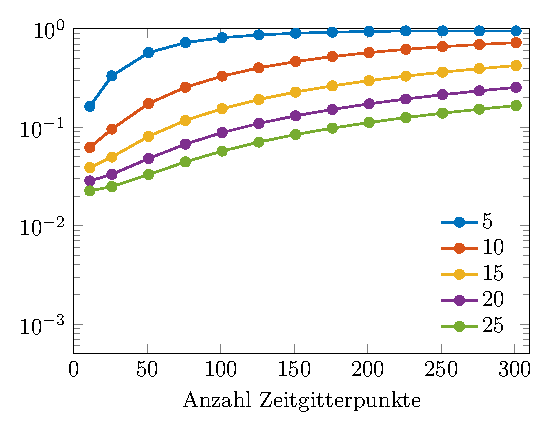
\includegraphics[width=1\textwidth]{figures/chapter4/stability_sine_dataset1_fig_1.pdf}
        \caption{Exakte inf-sup-Konstante $\beta_{\mathcal N}$.}
    \end{subfigure}
    \begin{subfigure}[b]{0.495\textwidth}
        \centering
        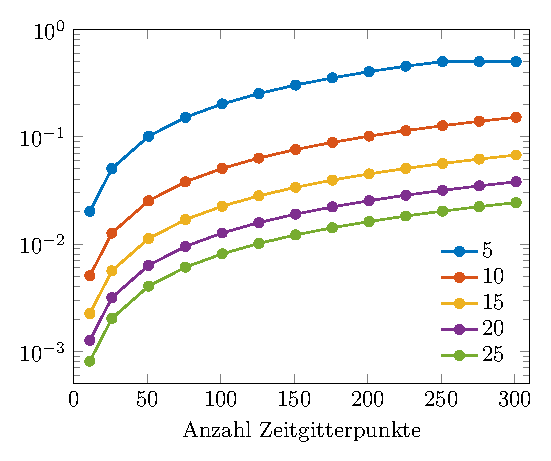
\includegraphics[width=1\textwidth]{figures/chapter4/stability_sine_dataset1_fig_2.pdf}
        \caption{Untere Schranke nach \cref{satz:untere_schranke_fuer_infsup_nach_andreev}.}
    \end{subfigure}
    \caption[Stabilität der Diskretisierung mit homogenen Randbedingungen, erstes Beispiel.]{%
        Zur Stabilität der Diskretisierung des ersten Beispiels.
        Die Farben repräsentieren dabei die verschiedenen Werte für die Dimension $\mathcal J$ der räumlichen Diskretisierung $V_{\mathcal J}$, während auf der horizontalen Achse $\mathcal K$ aufgetragen ist.
        }
    \label{figure:infsup_homogen_ein_feld}
\end{figure}

Als erstes einfaches Modell betrachten wir die Propagator"=Differentialgleichung ohne zeitlichen Wechsel der Felder.
Konkret wählen wir $I = [0, 1]$ sowie $\Omega = [0, 1]$ und ferner den Differentialoperator $A(t) \equiv A \colon V \to V'$ als
\begin{equation}
    A \eta = - \Delta \eta + \eta + \sin(\pi \blank) \eta.
\end{equation}
Dies entspricht einer Verschiebung um $\mu = 1$ und einem zeitlich konstanten Feld $\omega \colon \Omega \to \mathbb{R}$, $\omega = \sin(\pi \blank)$ mit $\norm{\omega}_{L_{\infty}(I; L_{\infty}(\Omega))} = 1 = \mu$.
Damit wird in \cref{satz:bilinearform_messbar_stetig_garding} die G\aa{}rding-Ungleichung mit $\lambda = 0$ erfüllt und wir können die in \cref{satz:untere_schranke_fuer_infsup_nach_andreev} beschriebene untere Schranke für die inf-sup-Konstante $\beta_{\mathcal N}$ auswerten.

\cref{figure:infsup_homogen_ein_feld} zeigt sowohl die exakt bestimmte diskrete inf-sup-Konstante $\beta_{\mathcal N}$ als auch die untere Schranke für verschiedene Werte von $\mathcal J$ und $\mathcal K$.
Zwar kann an dieser Stelle die Konstante $c_{0}$ aus \cref{satz:untere_schranke_fuer_infsup_nach_andreev} nicht näher bestimmt werden, aber es ist auf den ersten Blick ersichtlich, dass die Schranke das tatsächliche Verhalten der inf-sup-Konstante qualitativ gut widerspiegelt.
Ferner wird die CFL"=Bedingung bekräftigt, da für festes $\mathcal J$ und wachsende Anzahl $\mathcal K$ an Zeitgitterpunkten die inf"=sup"=Konstante sich dem Wert $1$ von unten annähert.

Das zweite, etwas komplexere Beispiel enthält nun einen zeitlichen Wechsel bei $T_{f} = 0.5$.
Der Differentialoperator $A(t) \colon V \to V'$ sei gegeben durch
\begin{equation}
    \begin{aligned}
        A(t)\eta =
        &- \Delta \eta + 3 \eta + \chi_{[0, 0.5)}(t) \left[ \sin(\pi \blank) - \sin(3 \pi \blank) \right] \eta
        \\&+ \chi_{[0.5, 1]}(t) \left[ \sin(2 \pi \blank ) + \sin(3 \pi \blank) \right] \eta.
    \end{aligned}
\end{equation}
Erneut ist mit $\mu = 3$ sichergestellt, dass die G\aa{}rding"=Ungleichung mit $\lambda = 0$ erfüllt wird.
\cref{figure:infsup_homogen_zwei_felder} zeigt die Ergebnisse für diese Modelldaten.
Auffallend ist, das die resultierenden Werte nahezu identisch sind mit denen des einfachen Beispiels.
Dies ist dadurch bedingt, dass in beiden Beispielen die Verschiebung $\mu$ so gewählt wurde, dass der Differentialoperator $A(t)$ elliptisch wird.

\begin{figure}[p]
    \centering
    \centering
    \begin{subfigure}[b]{0.495\textwidth}
        \centering
        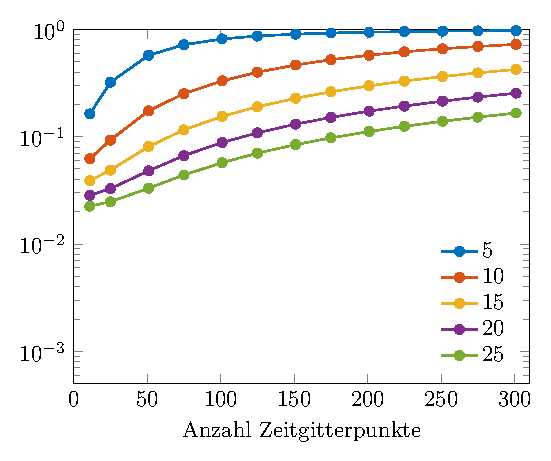
\includegraphics[width=1\textwidth]{figures/chapter4/stability_sine_dataset2_fig_1.pdf}
        \caption{Exakte inf-sup-Konstante $\beta_{\mathcal N}$.}
    \end{subfigure}
    \begin{subfigure}[b]{0.495\textwidth}
        \centering
        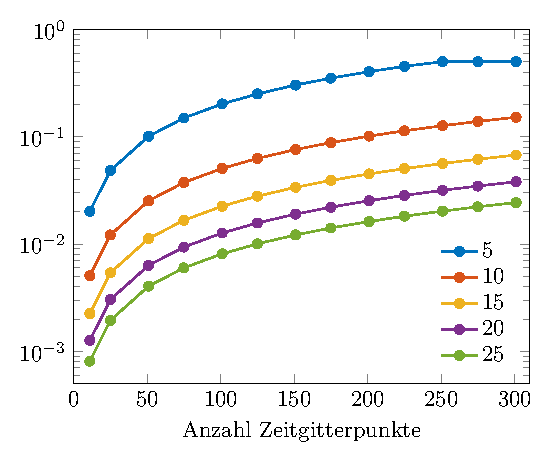
\includegraphics[width=1\textwidth]{figures/chapter4/stability_sine_dataset2_fig_2.pdf}
        \caption{Untere Schranke nach \cref{satz:untere_schranke_fuer_infsup_nach_andreev}.}
    \end{subfigure}
    \caption[Stabilität der Diskretisierung mit homogenen Randbedingungen, zweites Beispiel.]{%
        Ergebnisse des zweiten Beispiels mit homogenen Randbedingungen.
        Erneut repräsentieren die Farben die verschiedenen Werte für $\mathcal J$ und die horizontale Achse die Dimension $\mathcal K$.
        }
    \label{figure:infsup_homogen_zwei_felder}
\end{figure}

\paragraph{Periodische Randbedingungen.} % (fold)
\label{par:periodische_randbedingungen_}

Auch auf die periodischen Randbedingungen wollen wir an dieser Stelle kurz eingehen und das zweite Beispiel nun in diesem Setting noch einmal betrachten.
Dabei übernehmen wir die dortigen Gegebenheiten und passen lediglich die verwendete Diskretisierung $V_{\mathcal J}$ an.
Diese wählen wir erneut in Form eines Fourier-Ansatzes, diesmal als
\begin{equation}
    V_{\mathcal J} := \spn \Set{ v_{j} \given j = 1, \dots, \mathcal J}
\end{equation}
mit den Basisfunktionen
\begin{equation}
    v_{j} := \begin{cases}
        \cos(\pi (j - 1) \blank / L), & \text{falls } j \text{ ungerade},\\
        \sin(\pi j \blank / L), & \text{falls } j \text{ gerade}.
    \end{cases}
\end{equation}

Nach den Aussagen in \cref{section:periodische_randbedingungen} können wir ohne Transformation im Sinne von \cref{lemma:transformation_zu_elliptischem_operator} die G\aa{}rding-Ungleichung im Allgemeinen nicht mit $\lambda = 0$ erfüllen.
Wir verzichten an dieser Stelle darauf, da diese im Wesentlichen nur für die Invertierbarkeit des Operators $A(t)$ benötigt wird und diese, wie bei der numerischen Umsetzung deutlich wurde, ist hier bereits gegeben.

\begin{figure}[p]
    \centering
    \centering
    \begin{subfigure}[b]{0.495\textwidth}
        \centering
        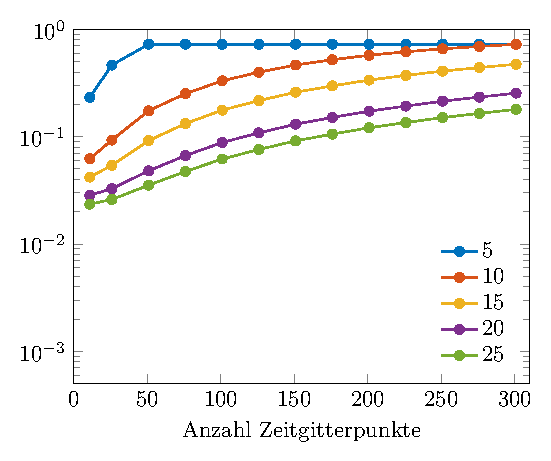
\includegraphics[width=1\textwidth]{figures/chapter4/stability_fourier_dataset1_fig_1.pdf}
        \caption{Exakte inf-sup-Konstante $\beta_{\mathcal N}$.}
    \end{subfigure}
    \begin{subfigure}[b]{0.495\textwidth}
        \centering
        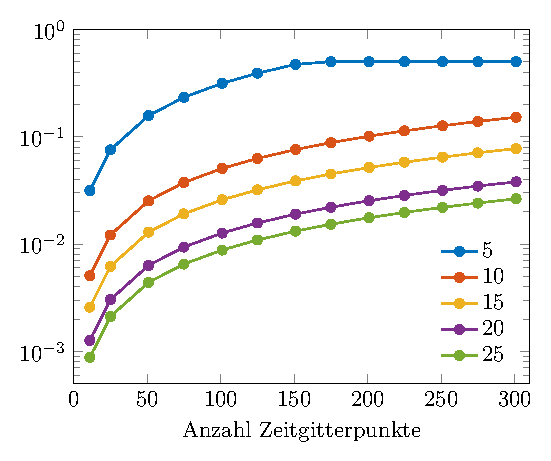
\includegraphics[width=1\textwidth]{figures/chapter4/stability_fourier_dataset1_fig_2.pdf}
        \caption{Untere Schranke nach \cref{satz:untere_schranke_fuer_infsup_nach_andreev}.}
    \end{subfigure}
    \caption[Stabilität der Diskretisierung mit periodisches Randbedingungen.]{%
        Ergebnisse des zweiten Beispiels im Falle periodischer Randbedingungen.
        }
    \label{figure:infsup_periodisch_zwei_felder}
\end{figure}

Die Ergebnisse sind in \cref{figure:infsup_periodisch_zwei_felder} zu sehen.
Diese weisen im Vergleich zum Fall homogener Randbedingungen nur kleine Differenzen auf und liefern sogar leicht bessere, das heißt größere, Werte bei der exakt bestimmten diskreten inf-sup-Konstante.

\paragraph{}
Sowohl im Fall homogener als auch periodischer Randbedingungen bekräftigen die vorliegenden Ergebnisse die Wahl der Diskretisierung.
Zwar handelt es sich dabei um relativ simple Modelle, allerdings legen diese bereits nahe, dass mit der Anpassung der Verschiebung $\mu$ der Felder ein Instrument zur Verfügung steht, mit dem auch in komplizierteren Fällen gute Stabilitätsergebnisse erzielt werden können.

\end{document}

    % % -*- root: ../main.tex -*-

\documentclass[../main.tex]{subfiles}
\begin{document}

\chapter{Reduzierte-Basis-Methode} % (fold)
\label{chapter:rbm}

% chapter reduzierte_basis_methode (end)

Nun wird aufbauend auf das Petrov-Galerkin-Verfahren des vorherigen Kapitels die Reduzierte-Basis-Methode eingeführt und auf das gegebene Setting übertragen.
Anschließend wird die numerische Umsetzung dieser für unsere bereits in \cref{section:galerkin_numerische_umsetzung_und_experimente} betrachtete Problemstellung angegangen und die Ergebnisse diskutiert.

\section{Grundlagen} % (fold)
\label{sub:grb:rb:grundlagen}

Wir beginnen mit einer kurzen Motivation und Einführung der Reduzierte"=Basis"=Methoden.
Dabei handelt es sich um ein relativ junges Verfahren, welches besonders in den letzten Jahren viel Aufmerksamkeit und Weiterentwicklung erfahren hat.
Eine weitaus umfassendere Einführung als die nachfolgende findet man beispielsweise in der Arbeit von \textcite{Patera:2007un}.

Um die Idee hinter der Reduzierte-Basis-Methode zu erklären, benötigen wir das folgende Setting: Sei $\mathcal P \subset \mathbb{R}^{p}$ eine abgeschlossene und konvexe Parametermenge und sei das folgende parametrische Variationsproblem gegeben:
Sei $\mu \in \mathcal P$, finde $u(\mu) \in \mathcal X$ mit
\begin{equation}
    \label{eq:rbm_varprob_allgemein}
    b(u(\mu), v; \mu) = f(v; \mu) \quad \fa v \in \mathcal Y,
\end{equation}
wobei $b(\blank, \blank; \mu) \colon \mathcal X \times \mathcal Y \to \mathbb{R}$ eine Bilinearform und $f(\blank; \mu) \colon \mathcal Y \to \mathbb{R}$ ein lineares Funktional ist, so dass für alle $\mu \in \mathcal P$ das obige Variationsproblem korrekt gestellt ist.
Probleme dieser Art werden oft, wie beispielsweise in \cref{chapter:galerkin} beschrieben, mittels Galerkin-Verfahren auf hochdimensionalen Räumen $\mathcal X^{\mathcal N}$ und $\mathcal Y^{\mathcal N}$ gelöst.
Wir stützen uns darauf, dass der Fehler dieser Diskretisierung theoretisch beliebig klein gehalten werden kann und bezeichnen im Folgenden die Räume $\mathcal X^{\mathcal N}$ und $\mathcal Y^{\mathcal N}$ als Truth-Ansatz- respektive Truth-Testraum und die entsprechende diskrete Lösung $u^{\mathcal N}(\mu) \in \mathcal X^{\mathcal N}$ als Truth-Lösung.

Unter der Annahme, dass die Lösung $u(\mu) \in \mathcal X$ eine gewissen Regularität bezüglich des Parameters $\mu \in \mathcal P$ aufweist, hat die durch die Lösungen gebildete Mannigfaltigkeit $\mathcal M^{\mathcal N} = \Set{u^{\mathcal N}(\mu) \in \mathcal X^{\mathcal N} \given \mu \in \mathcal P}$ meist eine eher niedrige Dimension, vergleiche \cref{fig:figure1}.
Hier setzen die Reduzierte-Basis-Methoden an; der Reduzierte-Basis-Ansatzraum $\mathcal X_{N}$ wird definiert als $N$-dimensionale Approximation
\begin{equation}
    \mathcal X_{N} = \spn\Set{u^{\mathcal N}(\mu_{i}) \given i = 1 \dots N} = \spn\Set{\xi_{1}, \dots, \xi_{N}}
\end{equation}
an $\mathcal M^{\mathcal N}$, wobei $N \ll \mathcal N$ wünschenswert ist.
Die Reduzierte-Basis-Lösung $u_{N}(\mu)$ wird dann durch erneute Galerkin-Projektion von \cref{eq:rbm_varprob_allgemein} auf $\mathcal X_{N}$ und einen noch näher zu bestimmenden Reduzierte-Basis-Testraum $\mathcal Y_{N}$ bestimmt.

\begin{figure}[tb]
    \centering
    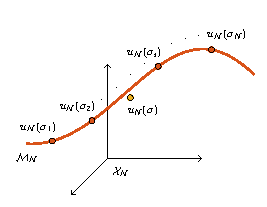
\includegraphics[width=0.6\textwidth]{figures/rb.pdf}
    \caption[%
    Skizze zur Motivation der Reduzierte-Basis-Methode.
    ]{
        Skizzenhafte Darstellung der Funktionsweise der Reduzierte-Basis-Methode.
        Die Reduzierte-Basis-Approximation $u_{N}(\mu)$ ergibt sich als Linearkombination der Finite-Elemente-Snapshots $u^{\mathcal N}(\mu_{i})$, welche mutmaßlich eine glatte parametrische Manigfaltigkeit bilden.
        }
    \label{fig:figure1}
\end{figure}


\section{Grundlagen pt. II} % (fold)
\label{sec:grundlagen}

Wir knüpfen an \cref{chapter:galerkin} an und betrachten zunächst ein abstraktes parametrisches Variationsproblem der Form
\begin{equation}
    \text{Sei } \bm \sigma \in \mathcal P, \text{ finde } u(\bm \sigma) \in \mathcal X \colon b(u(\bm \sigma), v; \bm \sigma) = f(v) \quad \fa v \in \mathcal Y.
\end{equation}
Für den Rest dieses Kapitels fordern wir, dass die Familie von Bilinearformen $b(\blank, \blank; \bm \sigma) \colon \mathcal X \times \mathcal Y \to \mahtbb{R}$ affin vom Parameter $\bm \sigma$ abhängt, genauer die Form
\begin{equation}
     b(\blank, \blank; \bm \sigma) = \sum_{q = 1}^{Q_b} \theta_{b}^{q}(\bm \sigma) b_{q}(\blank, \blank)
 \end{equation}
 mit parameterunabhängigen Bilinearformen $b_{q} \colon \mathcal X \times \mathcal Y \to \mathbb{R}$ und nicht näher spezifizierten Abbildungen $\theta_{b}^{q} \colon \mathcal P \to \mathbb{R}$ für $q = 1, \dots, Q_{b}$.

\begin{Definition}
    Seien $\mathcal X^{\mathcal N}$ und $\mathcal Y^{\mathcal N}$ zwei endlichdimensionale Räume einer Petrov-Galerkin-Diskretisierung und diese Diskretisierung sei durch das folgende Variationsproblem gegeben:
    \begin{equation}
        \text{Sei } \bm \sigma \in \mathcal P, \text{ finde } u^{\mathcal N}(\bm \sigma) \in \mathcal X^{\mathcal N} \colon \quad b(u^{N}(\bm \sigma), v; \bm \sigma) = f(v) \quad \fa v \in \mathcal Y.
    \end{equation}
    Ohne Einschränkung sei dieses Problem korrekt gestellt.
    Wir nennen die Lösung $u^{\mathcal N}(\bm \sigma)$ dieses diskreten Variationsproblems im folgenden \emph{Truth}-Lösung.
\end{Definition}

\begin{Definition}
    Sei $u_{N}(\bm \sigma) \in \mathcal X_{N}$ die Reduzierte-Basis-Lösung und $u^{\mathcal N}(\bm \sigma) \in \mathcal X^{\mathcal N}$ die Truth-Lösung.
    Wir definieren den \emph{Fehler} $e_{N}(\bm \sigma) \in \mathcal X^{\mathcal N}$ als
    \begin{equation}
        e_{N}(\bm \sigma) := u^{\mathcal N}(\bm \sigma) - u_{N}(\bm \sigma).
    \end{equation}
    Weiter definieren wir das \emph{Residuum} $r_{N}(\blank; \bm \sigma) \colon \mathcal Y^{\mathcal N} \to \mathbb{R}$ durch
    \begin{equation}
    \label{eq:variationsproblem_residuum}
        r_{N}(v; \bm \sigma) := b(e_{N}(\bm \sigma), v; \bm \sigma), \quad v \in \mathcal Y^{\mathcal N}.
    \end{equation}
\end{Definition}

\begin{Lemma}
    Das Residuum $r_{N}(\blank; \bm \sigma)$ ist für alle $\bm \sigma \in \mathcal P$ ein stetiges lineares Funktional, kurz also $r_{N}(\blank; \bm \sigma) \in \mathcal (\mathcal Y^{\mathcal N})'$.

    \begin{Beweis}
        Sowohl Linearität als auch Stetigkeit sind direkt ersichtlich, denn das Residuum kann nach Definition von $u^{\mathcal N}(\bm \sigma)$ geschrieben werden als
        \begin{equation}
            \begin{aligned}
            r_{N}(v; \bm \sigma)
            &= b(e_{N}(\bm \sigma), v; \bm \sigma)
            = b(u^{\mathcal N}(\bm \sigma), v; \bm \sigma) - b(u_{N}(\bm \sigma), v; \bm \sigma)
            \\&= f(v) - b(u_{N}(\bm \sigma), v; \bm \sigma).
            \end{aligned}
        \end{equation}
    \end{Beweis}
\end{Lemma}

Die $(\mathcal Y^{\mathcal N})'$-Norm des Residuums liefert uns nun ein brauchbares Maß für den Fehler zwischen Reduzierte-Basis- und Truth-Lösung.

\begin{Lemma}
    Sei $u_{N}(\bm \sigma) \in \mathcal X_{N}$ die Reduzierte-Basis-Lösung und $u^{\mathcal N}(\bm \sigma) \in \mathcal X^{\mathcal N}$ die Truth-Lösung.
    Dann gilt
    \begin{equation}
        \norm{u^{\mathcal N}(\bm \sigma) - u_{N}(\bm \sigma)}_{\mathcal X} \leq \frac{\norm{r_{N}(\blank; \bm \sigma)}_{(\mathcal Y^{\mathcal N})'}}{\beta_{\mathcal N}(\bm \sigma)}.
    \end{equation}

    \begin{Beweis}
        Da nach \cref{vorheriges Lemma} das Residuum ein Funktional auf $\mathcal Y^{N}$ ist, können wir \cref{eq:variationsproblem_residuum} als Variationsproblem auffassen, dessen eindeutige Lösung gerade $e_{N}(\bm \sigma)$ ist.
        Die Aussage folgt nun aus dem \acl{bnb}, \cref{satz:bnb_theorem}.
    \end{Beweis}
\end{Lemma}


\subsection{Bestimmung der inf-sup-Konstante} % (fold)
\label{sub:bestimmung_der_inf_sup_konstante}

Wie bei der Herleitung des Fehlers zwischen der Reduzierte-Basis-Lösung und der Truth-Lösung ersichtlich wurde, wird eine Möglichkeit benötigt die inf-sup-Konstante $\beta^{\mathcal N}(\mu)$ für viele verschiedene Parameter $\mu \in \mathcal P$ zu bestimmen, oder zumindest von unten zu beschränken.
Hierfür bietet sich die sogenannte \ac{SCM} an, welche speziell für die Anwendung bei Reduzierte-Basis-Methoden entwickelt wurde und eine sinnvolle Offline-Online-Zerlegung ermöglicht.

Wir orientieren uns dabei an dem Originalartikel von \textcite{Huynh2007} und den Verbesserungen von \textcite{Chen2009}.

Seien wie zuvor $\mathcal X^{\mathcal N}$ und $\mathcal Y^{\mathcal N}$ Ansatz- beziehungsweise Testraum des Truth"=Variationsproblems welches durch
\begin{equation}
0
\end{equation}


% subsection bestimmung_der_inf_sup_konstante (end)

% subsection grundlagen (end)

\section{Numerische Umsetzung} % (fold)
\label{sub:grb:rb:numerische_umsetzung}

% subsection numerische_umsetzung (end)

% section reduzierte_basis_methode (end)

% chapter reduzierte_basis_methode (end)

\end{document}

    % % -*- root: ../main.tex -*-

\documentclass[../main.tex]{subfiles}
\begin{document}

\chapter{Fazit \& Ausblick} % (fold)
\label{chapter:ausblick}

In diesem abschließenden Kapitel wollen wir die Ergebnisse dieser Arbeit noch einmal diskutieren.
Dabei betrachten wir diese hauptsächlich unter dem Aspekt der Anwendbarkeit auf die aus der \nameref{chapter:einleitung} bekannte selbstkonsistente Feldtheorie.

Analog zum Aufbau der Arbeit beginnen wir mit den funktionalanalytischen Ergebnissen aus \cref{chapter:propagator_differentialgleichung}, bevor wir weiter auf die zugrundeliegende Diskretisierung mittels \nameref{chapter:galerkin} und zuletzt auf die darauf aufbauende \nameref{chapter:rbm} eingehen.

\paragraph{Funktionalanalytische Ergebnisse.} % (fold)
\label{par:funktionalanalytische_ergebnisse}

\cref{chapter:propagator_differentialgleichung} lässt sich, neben der Herleitung der parametrischen Raum"=Zeit"=Variationsformulierung für die Propagator"=Differentialgleichung, zu den folgenden beiden Hauptergebnissen zusammenfassen:

\begin{enumerate}[label={\itshape\roman*.},ref={\itshape\roman*}]
    \item
    Der Nachweis, dass die hergeleitete Raum"=Zeit"=Variationsformulierung ein im Sinne von Hadamard korrekt gestelltes Problem darstellt.
    \item
    Die Untersuchung der Regularität der Lösungen der parametrischen Raum"=Zeit"=Variationsformulierung bezüglich der Parameter.
    Dabei wurde insbesondere eine hinreichende Bedingung dafür angegeben, wann diese Abhängigkeit analytisch ist.
\end{enumerate}

Vor allem der zweite Punkt bietet noch Potenzial für weitere Untersuchungen.
Die im Rahmen dieser Arbeit hergeleitete hinreichende Bedingung (siehe \cref{satz:loesungen_analytisch}) erweist sich als äußerst restriktiv, da sie maßgeblich festlegt, wie groß die Amplitude der verwendeten Felder sein darf und die zu erfüllende Schranke relativ niedrig ist.

Inwiefern dieses Ergebnis mit dem Ziel der analytischen Regularität verbessert werden kann, ist an dieser Stelle unklar.
Im Rahmen der Forschungsphase für das erzielte Ergebnis wurden verschiedene Ansätze verfolgt, die im Endeffekt alle zu einer ähnlich einschränkenden hinreichenden Bedingung führten.

Alternativ kann der Anspruch an die Regularität verringert werden, da Analytizität für die Anwendung der Reduzierte"=Basis"=Methode zwar gut, aber nicht notwendig ist.
Aufgrund der erzielten Ergebnisse liegt es nahe, dass schwächere Regularitätsergebnisse unter deutlich angenehmeren Bedingungen erreicht werden können.

\paragraph{Petrov-Galerkin-Diskretisierung.} % (fold)
\label{par:petrov_galerkin_diskretisierung}

In \cref{chapter:galerkin} wurde eine Diskretisierung durchgeführt, die als Grundlage für die Reduzierte"=Basis"=Methode verwendbar ist.
Weiter wurde eine hinreichende CFL"=Bedingung angegeben, unter welcher diese Diskretisierung stabil ist.

Auch hier bietet sich weiteres Verbesserungspotenzial.
Als erste einfache Verbesserung bietet es sich an, bei der numerischen Umsetzung die Raum"=Zeit"=Struktur stärker zu nutzen.
So müssen die vorkommenden Kronecker"=Produkte nicht zu $\mathcal N$-dimensionalen Objekten ausgewertet werden, da viele Berechnungen, die auf diesen Objekten basieren, durch Äquivalenzaussagen zu Berechnungen in den Dimensionen $\mathcal K$ und $\mathcal J$ überführt werden können.

Eine deutlich weiter ausholende Option ist, ein bedingungslos stabiles Verfahren zu konstruieren.
\textcite[Section 5.2]{Andreev:2012ep} hat gezeigt, dass die CFL"=Bedingung für das verwendete Verfahren möglicherweise verbessert, aber im Allgemeinen nicht entfernt werden kann.
Eine einfache Variante, um aus dem vorliegenden Verfahren ein bedingungslos stabiles zu erhalten, ist es, für den Testraum eine verfeinerte Zeitdiskretisierung zu verwenden.
Teilt man die Zeitgitterintervalle des Ansatzraumes für den Testraum jeweils in der Mitte auf, so führt dies zu bedingungsloser Stabilität.
Als Problem erweist sich nun aber, dass das resultierende System in Ansatz- und Testraum nicht mehr die gleiche Dimension besitzt und dementsprechend nur noch als Residuum"=minimierendes Variationsproblem aufgefasst werden kann.
Dieses kann aber nicht mehr als Grundlage für die Reduzierte"=Basis"=Methode verwendet werden.

Es bleibt zu untersuchen, ob und wie das verwendete Verfahren optimiert oder möglicherweise durch ein \enquote{besseres} Petrov"=Galerkin"=Verfahren ersetzt werden kann.

\paragraph{Reduzierte"=Basis"=Methode.} % (fold)
\label{par:reduzierte_basis_methode}

Als nächster Schritt wurde in \cref{chapter:rbm} die Reduzierte"=Basis"=Methode eingeführt.
Die theoretischen Grundlagen können zwar kurz gefasst werden, nichtsdestotrotz weist dieses Verfahren verschiedene verbesserungswürdige Punkte auf.

Wir beschränken uns auf den nach den Beispielen in \cref{sec:cha5_rbm:beispiele} offensichtlichen Ansatzpunkt, die Berechnung einer unteren Schranke für die parameterabhängige inf"=sup"=Konstante.
Dies stellt ein Kernstück der Reduzierte"=Basis"=Methode dar und wurde hier mit der \acl{scm} angegangen.
Dabei hat sich herausgestellt, dass diese stark unter dem Fluch der Dimensionalität leidet.
Ist die \ac{scm} bei einem Parameter noch in wenigen Minuten ausführbar, so benötigt sie bereits bei einer Parameterzahl im mittleren einstelligen Bereich mehrere Stunden.


Um dies zu verbessern, bietet sich zum einen die Verwendung einer optimierten \ac{scm}-Variante an wie beispielsweise \cite{Huynh2010}.
Zum anderen können möglicherweise die Schranken nach \cite{Schwab:2009ec} (siehe \cref{korrolar:ss09:theorem51_abschaetzungen}) als Ersatz zur \ac{scm} verwendet werden.
Für Letzteres bleibt aber zunächst die Exaktheit dieser Schranken zu untersuchen.
Spiegelt die Abschätzung das Verhalten der exakten inf"=sup"=Konstanten nur unzureichend wider, dann verfälscht dies insbesondere die Resultate des verwendeten Greedy"=Verfahrens.

Auch das Greedy-Iterationsverfahren der Reduzierte"=Basis"=Methode scheint stark unter der Erhöhung der Parameterdimension zu leiden, liefert hier aber nur bedingt aussagekräftige Ergebnisse, da die Bestimmung der inf-sup-Konstanten die weitere Analyse für höhere Dimensionen erschwert.

\paragraph{Selbstkonsistente Feldtheorie.} % (fold)
\label{par:selbstkonsistente_feldtheorie}

Als größter offener Punkt verbleibt die Frage, wie die in dieser Arbeit vorgestellte Modellreduktion verwendet werden kann, um die Berechnungen im Rahmen der selbstkonsistenten Feldtheorie zu beschleunigen.

Die vergleichsweise einfachste Option stellt die Substitution des in der \nameref{chapter:einleitung} beschriebenen Differentialgleichung"=Lösers im iterativen Verfahren durch die konstruierte Reduzierte"=Basis"=Methode dar.
Diese erfordert in der aktuellen Umsetzung a priori relativ tiefgehende Informationen, beispielsweise Symmetrien, über die resultierenden stabilen Felder, da sonst die Dimension des verwendeten Parameterraumes unpraktikabel groß wird.
Weiter muss hierfür bei Änderung der Modellparameter vor dem iterativen Verfahren stets zunächst der Offline-Anteil der Reduzierte"=Basis"=Methode ausgeführt werden, was bei aktueller Umsetzung jegliche mögliche Zeiteinsparung durch die Modellreduktion zerstört.

Um auf solches a priori-Wissen verzichten zu können, ist eine dynamische Reduzierte"=Basis"=Methode gefragt, die nicht einfach nur als Löser"=Ersatz für die Propagator"=Differentialgleichungen verwendet wird.
Diese sollte nach Möglichkeit direkt mit dem iterativen Verfahren gekoppelt sein und während der Ausführung \enquote{lernen}, welche Funktionen ein zur Modellreduktion der Felder geeignetes System darstellen.

Unseres Wissens wurden dynamische Reduzierte"=Basis"=Methoden dieser Art bisher nicht untersucht und stellen damit einen größeren, noch unerforschten Bereich dar.

\end{document}


    % % % -*- root: ../main.tex -*-

\iftoggle{dictum}{
    \setchapterpreamble[ul][0.6\textwidth]{%
        \dictum[Robert Heinlein, \textit{Time Enough For Love}]{\enquote{Progress isn't made by early risers. It's made by lazy men trying to find easier ways to do something.}}
        \vspace*{2\baselineskip}
    }
}{}
\chapter{Der eindimensionale Fall}
\label{sec:der_eindimensionale_fall}
\label{cha:der_eindimensionale_fall}

\todo[inline]{Kapitel ordentlich überarbeiten. Mittlerweile besser, aber noch deutlich verbesserungswürdig!}
\todo[inline]{Sind ein paar notationelle Kleinigkeiten zu korrigieren, also mal ordentlich durchlesen!}
\todo[inline]{Die Abschätzung in Satz 4.4. ist schon heftig. Da bleibt ja so gut wie kein Spielraum für den Faktor K...}

In diesem Kapitel beschränken wir uns zunächst auf den vereinfachten Fall einer Raumdimension.
Es sei also $\Omega \subset \mathbb{R}$ ein Intervall.
Ohne Beschränkung der Allgemeinheit wählen wir $\Omega = [0, L]$ für ein $0 < L < \infty$.

\todo[inline]{Eventuell wäre, insbesondere mit der gewünschten Anwendung bei SCFT-Verfahren, eine Entwicklung in Cosinus-Funktionen (oder direkt Fourier-Reihen) sinnvoller.
Insbesondere wären Cosinus-Funktionen achsensymmetrisch und automatisch nicht-homogen; beides Eigenschaften, welche die Felder $\omega$ bei der SCFT oftmals aufweisen.}


Als Ansatzfunktionen für eine geeignete Entwicklung des Operators $A$ in eine affin parametrische Darstellung wählen wir Sinusfunktionen, welche zusätzlich gewichtet werden, so dass wir die gewünschten Konvergenzeigenschaften erhalten.
Zusätzlich zu den Sinusfunktionen fügen wir eine konstante Funktion $\varphi_{0}$ hinzu, um so inhomogene Randbedingungen für $\omega$ zuzulassen.

Da die Parameter $\sigma$ weiterhin aus der Menge $\mathcal S = [-1, 1]^{\mathbb{N}}$ kommen, skalieren wir die Ansatzfunktionen mit einem Faktor $K \in \mathbb{R}_{+}$.
Dieser Faktor wird später durch die Anforderungen, die wir durch die gewünschte analytische Abhängigkeit vom Parameter erhalten, genauer bestimmt.

Konkret kommt nun
\begin{equation}
    \label{eq:sinusfunktionen_ansatz}
    \varphi_{0} = K, \qquad
    \varphi_{j} = \frac{K}{(\pi j)^{1 + \epsilon}} \sin(\tfrac{\pi j}{L} \blank), \quad j \geq 1,
\end{equation}
als Funktionensystem $\Set{ \varphi_{j} }_{j \geq 0}$ zum Einsatz.
Damit schreiben wir den parametrischen Faktor $\omega$ der linearen Evolutionsgleichung aus dem vorherigen Kapitel als
\begin{equation}
    w(\blank; \sigma) \colon \Omega \to \mathbb{R}, \quad w(x; \sigma) = \sum_{j = 0}^{\infty} \sigma_{j} \varphi_{j}(x)
\end{equation}
mit $\sigma \in \mathcal S$.
Damit schreibt sich die affine Zerlegung des Differentialoperators $A = - c \Delta + \omega$ als
\begin{equation}
    A = \hat A + \sum_{j = 0}^{\infty} \sigma_{j} A_{j}
\end{equation}
mit
\begin{equation}
    \label{eq:1d:affine_zerlegung}
    \hat A = - c \Delta, \qquad A_{j} = \varphi_{j}
\end{equation}
und den zugehörigen Bilinearformen
\begin{equation}
    \hat a(\eta, \zeta) = c \skprod{\grad \eta}{\grad \zeta}_{L_{2}(\Omega)}, \qquad a_{j}(\eta, \zeta) = \skprod{\varphi_{j} \eta}{\zeta}_{L_{2}(\Omega)}.
\end{equation}


Zunächst rechnen wir nun verschiedene, später benötigte, Normen nach.
\begin{Lemma}
    Es gilt
    \begin{alignat}{2}
        \norm{\varphi_{0}}_{L_{\infty}(\Omega)} &= K,
        \qquad&
        \norm{\varphi_{j}}_{L_{\infty}(\Omega)} &= \frac{K}{(\pi j)^{1 + \epsilon}} , \quad j \geq 1,
    \intertext{sowie}
        \norm{\varphi_{0}}_{H^{1}(\Omega)}  &= K \sqrt{L},
        \qquad&
        \norm{\varphi_{j}}_{H^{1}(\Omega)}  &= \frac{K \sqrt{L^{2} + (\pi j)^{2}}}{\sqrt{2L} (\pi j)^{1 + \epsilon}}
        , \quad j \geq 1.
    \end{alignat}
\end{Lemma}

\begin{Lemma}
    Die Funktionen $\Set{ \varphi_{j} }_{j \geq 1}$ bilden ein Orthogonalsystem in $H^{1}(\Omega)$, denn es gilt
    \begin{equation}
        \skprod{\varphi_{j}}{\varphi_{k}}_{H^{1}(\Omega)} = \begin{cases}
            \frac{K^{2}}{2L} \frac{L^{2} + (\pi j)^{2}}{(\pi j)^{2(1 + \epsilon)}}
            ,   &j = k \\
            0,          &j \neq k.
        \end{cases}
    \end{equation}
\end{Lemma}

\begin{Lemma}
    Sei $\sigma \in \mathcal S$ und $\epsilon > 0$, dann konvergiert obiges $\omega(\blank; \sigma)$ in $L_{\infty}(\Omega)$.
    Ist $\epsilon > 1$, dann gilt auch Konvergenz in $H^{1}_{0}(\Omega)$.

    \begin{Beweis}
        Sei zunächst $\epsilon > 0$.
        Da $\mathcal S = [0, 1]^{\mathbb{N}}$ ist, erhalten wir die Konvergenz in $L_{\infty}(\Omega)$ nach dem Weierstraßschen Majorantenkriterium via
        \begin{align}
            \sum_{j = 0}^{\infty} \norm{\sigma_{j} \varphi_{j}}_{L_{\infty}(\Omega)}
            &= \sum_{j = 0}^{\infty} \abs{\sigma_{j}} \norm{\varphi_{j}}_{L_{\infty}(\Omega)}
             \leq \norm{\varphi_{0}}_{L_{\infty}(\Omega)} + \sum_{j = 1}^{\infty}  \norm{\varphi_{j}}_{L_{\infty}(\Omega)}
            \\&= K + \sum_{j = 1}^{\infty} \frac{K}{(\pi j)^{1 + \epsilon}}
            = K + \frac{K}{\pi^{1 + \epsilon}} \sum_{j = 1}^{\infty} \frac{1}{j^{1+\epsilon}}
        \end{align}
        Diese Reihe konvergiert bekanntlich für alle $\epsilon > 0$, womit wir bereits die Konvergenz von $\omega$ in $L_{\infty}(\Omega)$ erhalten.

        Sei nun $\epsilon > 1$.
        Betrachte
        \begin{align}
            \sum_{j = 0}^{\infty} \norm{\sigma_{j} \varphi_{j}}_{H^{1}(\Omega)}
            &= \sum_{j = 0}^{\infty} \abs{\sigma_{j}} \norm{\varphi_{j}}_{H^{1}(\Omega)}
            \leq  \norm{\varphi_{0}}_{H^{1}(\Omega)} + \sum_{j = 1}^{\infty} \norm{\varphi_{j}}_{H^{1}(\Omega)}
            \\&= K \sqrt{L} + \sum_{j = 1}^{\infty} \frac{K \sqrt{L^{2} + (\pi j)^{2}}}{\sqrt{2L} (\pi j)^{1 + \epsilon}}
            \\&= K \sqrt{L} + \frac{K}{\sqrt{2L}} \sum_{j = 1}^{\infty} \frac{\sqrt{L^{2} + (\pi j)^{2}}}{(\pi j)^{1 + \epsilon}}
            \\&\leq K \sqrt{L} + \frac{K}{\sqrt{2L}} \sum_{j = 1}^{\infty} \frac{L + \pi j}{(\pi j)^{1 + \epsilon}}
            \\&= K \sqrt{L} + \frac{K}{\sqrt{2L}} \sum_{j = 1}^{\infty} \frac{L}{(\pi j)^{1 + \epsilon}} + \frac{K}{\sqrt{2L}} \sum_{j = 1}^{\infty} \frac{1}{(\pi j)^{\epsilon}}
        \end{align}
        Wegen $\epsilon > 1$ konvergiert sowohl die erste als auch die zweite Reihe.
        Zusammen liefert dies die Konvergenz in $H^{1}_{0}(\Omega)$.
    \end{Beweis}
\end{Lemma}

Wir wollen nun die Regularität von $\omega(\blank; \sigma)$ in Abhängigkeit vom Parameter $\sigma$ nachweisen.

\todo[inline]{Anpassen! Lässt sich die Schranke verbessern?}
\begin{Satz}
\label{satz:regularitaet_nachrechnen}
    Seien $\epsilon > 0$ und $0 < \kappa < 1$ so gewählt, dass
    \begin{equation}
        \sum_{j = 1}^{\infty} \frac{1}{j^{2 + \epsilon}} \leq \frac{(\kappa c (\tfrac{\pi}{L})^{2} - K) \pi^{2 + \epsilon}}{4 C_{\infty} K L^{3/2}}
    \end{equation}
    gilt,
    wobei $c$ und $K$ die Konstanten aus \eqref{eq:def_op_A} respektive \eqref{eq:sinusfunktionen_ansatz} und $C_{\infty}$ die Einbettungskonstante von $H^{1}_{0}(\Omega) \hookrightarrow L_{\infty}(\Omega)$ sind.
    Dann erfüllt die affine Zerlegung $\Set{\hat A, A_{j} \given j \in \mathbb{N}_{0}}$ \thref{thm:kunoth:assumption2}.

    \begin{Beweis}
        Wir weisen zunächst die inf-sup-Bedingungen \eqref{eq:kunoth:ass2_gamma_0} für $\hat a(\blank, \blank)$ nach und bestimmen die Konstante $\gamma_{0}$.
        Da $\hat a(\blank, \blank)$ symmetrisch ist, genügt es, die inf-sup-Bedingung \eqref{eq:kunoth:ass2_gamma_0_a} nachzuweisen. Die zweite inf-sup-Bedingung \eqref{eq:kunoth:ass2_gamma_0_b} folgt dann analog mit dem selben $\gamma_{0}$.

        Nach \thref{lem:sauter:2.1.48} reicht es, für alle $\eta \in H^{1}_{0}(\Omega)$ ein $\zeta = \zeta(\eta) \in H^{1}_{0}(\Omega)$ und von $\eta$ und $\zeta$ unabhängige Konstanten $C_{1}, C_{2} > 0$ mit
        \begin{equation}
            \hat a(\eta, \zeta) \geq C_{1} \norm{\eta}_{H^{1}(\Omega)}^{2} \quad \text{und} \quad \norm{\zeta}_{H^{1}(\Omega)} \leq C_{2} \norm{\eta}_{H^{1}(\Omega)}
        \end{equation}
        zu finden.
        Dann ist die inf-sup-Bedingung \eqref{eq:kunoth:ass2_gamma_0_a} mit $\gamma_{0} = \frac{C_{1}}{C_{2}}$ erfüllt.

        Sei nun also $\eta \in H^{1}_{0}(\Omega)$ beliebig.
        Wir wählen $\zeta = \eta \in H^{1}_{0}(\Omega)$, das heißt, es gilt $C_{2} = 1$.
        Es ergibt sich
        \begin{align}
            \hat a(\eta, \zeta) = \hat a(\eta, \eta) = c \skprod{\grad \eta}{\grad \eta}_{L_{2}(\Omega)} = c \norm{\grad \eta}_{L_{2}(\Omega)}^{2} \geq c \gamma_{\Omega}^{2} \norm{\eta}_{H^{1}(\Omega)}^{2},
        \end{align}
        wobei die letzte Abschätzung aus der Poincaré-Friedrichs-Ungleichung \eqref{eq:gl:poincare_friedrichs_ungleichung} folgt.
        Zusammen liefert dies $\gamma_{0} = c \gamma_{\Omega}^{2}$ als inf-sup-Konstante.

        Für den vorliegenden Fall können wir $\gamma_{\Omega}^{2}$ exakt bestimmen.
        Nach \cite[Chapter 11]{Strauss:2007vz} entspricht das Quadrat der optimalen Poincaré-Friedrichs-Konstante $\gamma_{\Omega}^{2}$ gerade dem kleinsten Eigenwert des Laplace-Operators auf $\Omega$ mit Dirichlet-Randbedingung.
        Dieser hat für $\Omega = [0, L]$ den Wert $\frac{\pi^{2}}{L^{2}}$.
        Wir erhalten damit also $\gamma_{0} = c \frac{\pi^{2}}{L^{2}}$.

        Seien nun $\eta, \zeta \in H^{1}_{0}(\Omega)$.
        Für $j = 0$ gilt die simple Abschätzung
        \begin{equation}
            \begin{aligned}
                a_{0}(\eta, \zeta)
                &= \skprod{\varphi_{0} \eta}{\zeta}_{L_{2}(\Omega)}
                = K \skprod{\eta}{\zeta}_{L_{2}(\Omega)}
                \\&\leq K \norm{\eta}_{L_{2}(\Omega)} \norm{\zeta}_{L_{2}(\Omega)}
                \leq K \norm{\eta}_{H^{1}(\Omega)} \norm{\zeta}_{H^{1}(\Omega)}
            \end{aligned}
        \end{equation}
        Betrachte für $j \geq 1$
        \begin{align}
            a_{j}(\eta, \zeta)
            &= \skprod{\varphi_{j} \eta}{\zeta}_{L_{2}(\Omega)}
            = \int_{0}^{L} \varphi_{j} \eta \zeta \diff x
            \intertext{da $\varphi_{j}$ integrierbar ist und $\varphi_{j}(0) = 0$, können wir dies umschreiben zu}
            a_{j}(\eta, \zeta)
            &= \int_{0}^{L} \frac{\diff}{\diff x} \left( \int_{0}^{x} \varphi_{j}(y) \diff y \right) \eta \zeta \diff x
            \intertext{woraus wir mittels partieller Integration und $\eta, \zeta \in H^{1}_{0}(\Omega)$ folgenden Ausdruck erhalten}
            a_{j}(\eta, \zeta)
            &= - \int_{0}^{L} \left( \int_{0}^{x} \varphi_{j}(y) \diff y \right) (\eta \zeta)' \diff x
            \leq \norm*{\left( \int_{0}^{x} \varphi_{j}(y) \diff y \right) (\eta \zeta)'}_{L_{1}(\Omega)}
            \\&\leq \norm*{\int_{0}^{x} \varphi_{j}(y) \diff y }_{L_{\infty}(\Omega)} \norm{(\eta \zeta)'}_{L_{1}(\Omega)}.
        \end{align}
        Die erste Norm können wir weiter abschätzen mit
        \begin{equation}
            \begin{aligned}
                \norm*{\int_{0}^{x} \varphi_{j}(y) \diff y }_{L_{\infty}(\Omega)}
                &= \norm*{\int_{0}^{x} \frac{K}{(\pi j)^{1 + \epsilon}} \sin(\tfrac{\pi j}{L} y) \diff y}_{L_{\infty}(\Omega)}
                \\&= \norm*{\frac{K L}{(\pi j)^{2 + \epsilon}} \left( 1 - \cos(\tfrac{\pi j}{L} x) \right) }_{L_{\infty}(\Omega)}
                \leq \frac{2 K L}{(\pi j)^{2 + \epsilon}}
            \end{aligned}
        \end{equation}
        Aus der zweiten Norm erhalten wir mittels Minkowski- und Hölderungleichung sowie der Einbettung $H^{1}_{0}(\Omega) \hookrightarrow L_{\infty}(\Omega)$ die Abschätzung
        \begin{equation}
            \begin{aligned}
                \norm{(\eta \zeta)'}_{L_{1}(\Omega)}
                &= \norm{\eta' \zeta + \eta \zeta'}_{L_{1}(\Omega)}
                \leq \norm{\eta' \zeta}_{L_{1}(\Omega)} + \norm{\eta \zeta'}_{L_{1}(\Omega)}
                \\&\leq \norm{\eta'}_{L_{1}(\Omega)} \norm{\zeta}_{L_{\infty}(\Omega)} + \norm{\eta}_{L_{\infty}(\Omega)} \norm{\zeta'}_{L_{1}(\Omega)}
                \\&\leq \norm{1}_{L_{2}(\Omega)} \norm{\eta'}_{L_{2}(\Omega)} \norm{\zeta}_{L_{\infty}(\Omega)} + \norm{\eta}_{L_{\infty}(\Omega)} \norm{1}_{L_{2}(\Omega)} \norm{\zeta'}_{L_{2}(\Omega)}
                \\&\leq \sqrt{L} C_{\infty} \norm{\eta'}_{L_{2}(\Omega)} \norm{\zeta}_{H^{1}(\Omega)} + \sqrt{L} C_{\infty} \norm{\eta}_{H^{1}(\Omega)} \norm{\zeta'}_{L_{2}(\Omega)}
                % \\&\leq \norm{\eta'}_{L_{2}(\Omega)} \norm{\zeta}_{L_{2}(\Omega)} + \norm{\eta}_{L_{2}(\Omega)} \norm{\zeta'}_{L_{2}(\Omega)}
                \\&\leq 2 \sqrt{L} C_{\infty} \norm{\eta}_{H^{1}(\Omega)} \norm{\zeta}_{H^{1}(\Omega)}
            \end{aligned}
        \end{equation}
        Zusammen also
        \begin{align}
            a_{j}(u, v)
            &\leq \norm*{\int_{0}^{x} \varphi_{j}(y) \diff y }_{L_{\infty}(\Omega)} \norm{(\eta \zeta)'}_{L_{1}(\Omega)}
            \\&\leq \frac{4 K L^{3 / 2} C_{\infty}}{(\pi j)^{2 + \epsilon}} \norm{\eta}_{H^{1}(\Omega)} \norm{\zeta}_{H^{1}(\Omega)}.
        \end{align}
        Betrachte nun
        \begin{align}
                    \sum_{j = 0}^{\infty} \norm{A_{j}}_{\mathcal L(V, V')}
            &= \norm{A_{0}}_{\mathcal L(V, V')} + \sum_{j = 1}^{\infty} \norm{A_{j}}_{\mathcal L(V, V')}
            \\&\leq K + \sum_{j = 1}^{\infty} \frac{4 K L^{3 / 2} C_{\infty}}{(\pi j)^{2 + \epsilon}}
            \\&\leq K + \frac{4 K L^{3 / 2} C_{\infty}}{\pi^{2+ \epsilon}} \sum_{j = 1}^{\infty} \frac{1}{j^{2 + \epsilon}}
        \end{align}
        Fordern wir nun die Gültigkeit von \eqref{eq:kunoth:ass2_abs_reihe}, also
        \begin{equation}
            \sum_{j \geq 0} \norm{A_{j}}_{\mathcal L(V, V')} \leq \kappa \gamma_{0}
        \end{equation}
        für ein $0 < \kappa < 1$, dann ist damit also
        \begin{equation}
            \sum_{j = 1}^{\infty} \frac{1}{j^{2 + \epsilon}} \leq \frac{(\kappa (\tfrac{\pi}{L})^{2} - K) \pi^{2+ \epsilon}}{4 K L^{3/2} C_{\infty}}
        \end{equation}
        mit $\epsilon > 0$ hinreichend.
    \end{Beweis}
\end{Satz}

Zusammenfassend erhalten wir damit die folgende Aussage.

\todo[inline]{Besser ausformulieren}
\begin{Satz}
    Seien $\mathcal X$ und $\mathcal Y$ gegeben wie in~\eqref{eq:ps:rzvp:ansatzraum_testraum}.
    Weiter sei $\Set{\hat A, A_{j} \given j \in \mathbb{N}_{0}}$ die affine Zerlegung von $A = -c \Delta + \omega$ wie in \eqref{eq:1d:affine_zerlegung} und es gelte \thref{satz:regularitaet_nachrechnen}.
    Für jedes $\sigma \in \mathcal S$ sei $B(\sigma) \in \mathcal L(\mathcal X, \mathcal Y')$ definiert durch
    \begin{equation}
        \label{eq:ps:rg:theorem21_variationsproblem_als_operatorgleichung_parametrisch}
        \skprod{B(\sigma) u}{v}_{\mathcal Y' \times \mathcal Y} = b(u, v; \sigma), \quad u \in \mathcal X,~y \in \mathcal Y,
    \end{equation}
    mit $b(\blank, \blank; \sigma)$ wie in~\eqref{eq:ps:rzvp:schwache_formulierung_lhs_b_2}.
    Dann ist $B(\sigma)$ für jedes $\sigma \in \mathcal S$ stetig invertierbar und die parametrische Familie von Lösungen $u(\sigma)$ des parametrischen Raum-Zeit-Variationsproblems \eqref{eq:ps:rzvp:schwache_formulierung_2} hängt analytisch von $\sigma$ ab.

    \begin{Beweis}
        Direkte Folgerung aus \thref{satz:regularitaet_nachrechnen} und \thref{satz:ps:rg:kunoth13_theorem21}.
    \end{Beweis}
\end{Satz}

% subsection nachrechnen_von_thref_thm_kunoth_assumption2 (end)

% section der_eindimensionale_fall (end)

\clearpage
\section{Zu klärende Fragen} % (fold)
\label{sub:zu_kl_rende_fragen}

\begin{enumerate}
    \item Wohldefiniertheit der PDE \eqref{eq:parabolische_pde}, das heißt die Voraussetzungen von \thref{satz:gl:le:ss09_theorem51} nachweisen. Weiterhin lassen sich damit die inf-sup-Bedingung von \eqref{eq:ps:rzvp:schwache_formulierung} nachrechnen und damit die Schranken für $B$ und $B^{-1}$ bestimmen.
    \item Parametrische Variante des Variationsproblems herleiten.
    Dazu Ansetzen mit Entwicklung des Parameters $\omega$ in eine Reihe
    \begin{equation}
        \omega = \sum_{j = 0}^{\infty} \sigma_{j} \varphi_{j}.
    \end{equation}
    Dabei ergeben sich folgende Fragen:
    \begin{enumerate}
        \item Konvergenz der Reihe? Notwendig ist Konvergenz in $L_{\infty}(\Omega)$, da die Norm $\norm{\omega}_{L_{\infty}(\Omega)}$ mehrfach in Abschätzungen verwendet wird.
        \item Weiterhin ist eventuell Konvergenz in einem Unterraum $Z \hookrightarrow L_{\infty}(\Omega)$ wünschenswert.
        Zum Beispiel in $H^{1}(\Omega)$?
        \item Welche Bedingungen ergeben sich an $\sigma_{j}$ und $\varphi_{j}$?
        \item Welches Funktionensystem $\Set{ \varphi_{j} }_{j}$ ist überhaupt sinnvoll?
        Die Wahl der $\varphi_{j}$ entscheidet maßgeblich über Konvergenz der Reihenentwicklung.
        Welche Randvorgaben sind angestrebt?
        Dies wird ebenfalls durch die $\varphi_{j}$ geregelt.
    \end{enumerate}
    \item Welche affine Zerlegung $A(\sigma) = A_{0} + \sum_{j} \sigma_{j} A_{j}$ ist brauchbar?
    Wie genau sehen die $A_{j}$ aus?
    \item Nachweisen, dass $A(\sigma)$ \thref{ann:ps:rg:kunoth13_assumption1} oder \thref{thm:kunoth:assumption2} erfüllt und mittels \thref{satz:ps:rg:kunoth13_theorem21} die gewünschte Regularität von $B(\sigma)$ bezüglich $\sigma$ gewinnen.
    \item Die Abschätzungen in \thref{satz:regularitaet_nachrechnen} lassen sich noch deutlich verbessern.
    Das gilt wahrscheinlich auch für andere Abschätzungen!
\end{enumerate}


    % Alles, was noch unbedingt rein muss
    % % -*- root: ../main.tex -*-

\iftoggle{dictum}{
    \setchapterpreamble[ul][0.6\textwidth]{%
        \dictum[Terry Pratchett]{\enquote{Coffee is a way of stealing time that should by rights belong to your older self.}}
        \vspace*{2\baselineskip}
    }
}{}
\chapter{Funktionalanalytische Grundlagen} % (fold)
\label{cha:funktionalanalytische_grundlagen}

\todo[inline]{Ständig: ordnen, sortieren, aufräumen, erweitern.}

\section{Orthogonale Funktionen und Polynome}
\label{sec:orthogonale_funktionen_und_polynome}

\begin{Satz}[Orthogonalität trigonometrischer Funktionen]
\label{satz:trigonometrische_funktionen_orthogonal}
    Seien $k, l \in \mathbb{N}$.
    Dann gilt
    \begin{align}
        \skprod{\sin(\pi k x)}{\sin(\pi l x)}_{L_{2}([0, 1])} &= \frac{1}{2} \delta_{kl},
        % \quad\text{und}\quad
        \\\skprod{\cos(\pi k x)}{\cos(\pi l x)}_{L_{2}([0, 1])} &= \frac{1}{2} \delta_{kl},
        \\\skprod{\sin(\pi k x)}{\cos(\pi l x)}_{L_{2}([0, 1])} &= 0.
    \end{align}
\end{Satz}

\begin{Definition}[Legendre-Polynome]
\label{def:legendre_polynome}
    Sei $I = [-1, 1]$.
    Die Legendre-Polynome $L_{n} \in \Pi_{n}$ sind definiert durch
    \begin{equation}
        L_{n}(x) = \frac{1}{2^{n}n!}\frac{\diff^{n}}{\diff x^{n}} (x^{2} - 1)^{n}.
    \end{equation}
    Durch die Transformation $x \mapsto 2x - 1$ erhält man die auf das Interval $[0, 1]$ geshifteten Legendre-Polynome $\tilde L_{n}$.
\end{Definition}

\begin{Satz}[Orthogonalität der Legendre-Polynome]
\label{satz:legendre_polynome_orthogonal}
    Die Legendre-Polynome $L_{n}$ sind orthogonal bezüglich der $L_{2}([-1, 1])$-Norm, denn es gilt
    \begin{equation}
        \skprod{L_{n}}{L_{m}}_{L_{2}([-1, 1])} = \frac{2}{2n + 1} \delta_{n m}.
    \end{equation}
    Auch für die geshifteten Legendre-Polynome $\tilde L_{n}$ gilt Orthogonalität, denn es ist
    \begin{equation}
        \skprod{\tilde L_{n}}{\tilde L_{m}}_{L_{2}([0, 1])} = \frac{1}{2n + 1} \delta_{n m}.
    \end{equation}
\end{Satz}

\begin{Bemerkung}
\label{satz:legendre_polynome_rekursion}
    Die Legendre-Polynome $L_{n}$ erfüllen die Rekursionsformel
    \begin{equation}
        n L_{n}(x) = (2n - 1) x L_{n-1}(x) - (n - 1) L_{n-2}(x), \quad L_{0}(x) = 1, L_{1}(x) = x.
    \end{equation}
    Analog gilt für die erste Ableitung $L_{n}'$ die Rekursionsformel
    \begin{equation}
        (n - 1) L_{n}'(x) = (2n -1) x L_{n-1}'(x) - n L_{n-2}'(x), \quad L_{0}'(x) = 0, L_{1}'(x) = 1.
    \end{equation}
\end{Bemerkung}

\section{Sonstiges} % (fold)
\label{sec:sonstiges}

% \begin{Lemma}
%     $\mathcal C^{0}([a, b]; X)$ liegt dicht in $L_{p}(a, b; X)$ für $1 \leq p < \infty$.
% \end{Lemma}

% TODO: zitieren
\begin{Satz}[Poincaré-Friedrichs-Ungleichung, vgl. {{\cite[Lemma 89.4]{HankeBourgeois:2009fk}}}]
\label{satz:poincare_ungleichung}
    Sei $\Omega \subset \mathbb{R}^{n}$ offen, beschränkt und mit Lipschitz-Rand.
    Dann existiert eine Konstante $\gamma_{\Omega} > 0$ mit
    \begin{equation}
        \label{eq:gl:poincare_friedrichs_ungleichung}
        \norm{\grad u}_{L_{2}(\Omega)} \geq \gamma_{\Omega} \norm{u}_{H^{1}(\Omega)} \quad \fa u \in H^{1}_{0}(\Omega).
    \end{equation}
\end{Satz}

\begin{Satz}[Poincaré-Friedrichs-Ungleichung, vgl. {{\cite[Theorem II.1.7]{Braess:2007wm}}}]
    Es sei $\Omega \subset \mathbb{R}^{n}$ beschränkt und in einem $n$-dimensionalen Würfel mit Seitenlänge $s$ enthalten.
    Dann gilt
    \begin{equation}
        (1 + s)^{m} \abs{u}_{H^{m}} \geq \norm{u}_{H^{m}} \geq \abs{u}_{H^{m}} \quad \text{für alle}~u \in H^{m}_{0}(\Omega).
    \end{equation}
\end{Satz}

\begin{Lemma}[{{\cite[Remark 2.1.48]{Sauter:9_WoPZ0Y}}}]
\label{lem:sauter:2.1.48}
    Seien $X$ und $Y$ zwei reflexive Banachräume und $a \colon X \times Y \to \mathbb{R}$ eine Bilinearform.
    Finden wir für jedes $x \in X$ ein $y_{x} \in Y$, so dass
    \begin{equation}
        \label{eq:lem:sauter:2.1.48:eq1}
        \abs{a(x, y_{x})} \geq C_{1} \norm{x}_{X}^{2} \quad \text{und} \quad \norm{y_{x}}_{Y} \leq C_{2} \norm{x}_{X}
    \end{equation}
    mit von $x$ und $y_{x}$ unabhängigen Konstanten $C_{1}, C_{2} > 0$ gilt, dann folgt daraus die inf-sup-Bedingung
    \begin{equation}
    \label{eq:lem:sauter:2.1.48:inf_sup}
        \inf_{0 \neq x \in X} \sup_{0 \neq y \in Y} \frac{a(x, y)}{\norm{x}_{X}\norm{y}_{Y}} \geq \gamma > 0
    \end{equation}
    mit $\gamma = \frac{C_{1}}{C_{2}}$.

    \begin{Beweis}
        Seien $x \in X$ und $y_{x} \in Y$ so, dass \cref{eq:lem:sauter:2.1.48:eq1} erfüllt ist.
        Dann gilt
        \begin{align}
            \inf_{0 \neq x \in X} \sup_{0 \neq y \in Y} \frac{\abs{a(x, y)}}{\norm{x}_{X} \norm{y}_{Y}}
            &\geq
            \inf_{0 \neq x \in X} \frac{\abs{a(x, y_{x})}}{\norm{x}_{X} \norm{y_{x}}_{Y}}
            \\&\geq
            \inf_{0 \neq x \in X} \frac{C_{1} \norm{x}^{2}_{X}}{\norm{x}_{X} C_{2} \norm{x}_{X}}
            =
            \frac{C_{1}}{C_{2}}
            > 0.
        \end{align}
    \end{Beweis}
\end{Lemma}

% section sonstiges (end)

    % %!TEX root = ../main.tex

\chapter{Notizen} % (fold)
\label{cha:notizen}

% section zum_petrov_galerkin_verfahren (end)

\section{Reduzierte-Basis-Methode} % (fold)
\label{sec:reduzierte_basis_methode}

Bei der Reduzierte-Basis-Methode für die Raum-Zeit-Variationsformulierung parabolischer partieller Differentialgleichungen haben sich folgende Punkte ergeben, welche eine Anmerkung verdienen.

Seien dazu $\mathcal X^{\mathcal N} = \spn\Set{\phi_{n}}_{n=1}^{\mathcal N}$ und $\mathcal Y^{\mathcal M} = \spn\Set{\psi_{m}}_{m = 1}^{\mathcal M}$ endlichdimensionale Hilberträume, beispielsweise aus dem Petrov-Galerkin-Verfahren.
Im Allgeimeinen muss hier nicht $\mathcal N = \mathcal M$ gelten.
Weiter bezeichnen wir mit $\mathcal X_{N} \subset \mathcal X^{\mathcal N}$ und $\mathcal Y_{\mathcal M} \subset \mathcal Y_{M}$ die Reduzierte-Basis-Räume.

Wir betrachten das abstrakte Variationsproblem
\begin{equation}
    b(u, v; \mu) = f(v; \mu) \qquad \text{mit}~u \in \mathcal X,~v \in \mathcal Y,
\end{equation}
wobei $b \colon \mathcal X \times \mathcal Y \times \mathcal P \to \mathbb{R}$ eine affin parametrische Bilinearform und $f \colon \mathcal Y \times \mathcal P \to \mathbb{R}$ ein affin parametrisches lineares stetiges Funktional sei,
das heißt, es gelte
\begin{equation}
    b(u, v; \mu) = \sum_{q = 1}^{Q_b} \theta^{b}_{q}(\mu) b_{q}(u, v)
    \qquad \text{und} \qquad
    f(v; \mu) = \sum_{q = 1}^{Q_f} \theta^{f}_{q}(\mu) f_{q}(v).
\end{equation}

\paragraph{A posteriori Fehlerschätzer} % (fold)
\label{par:a_posteriori_fehlersch_tzer}

Der A-posteriori-Fehlerschätzer ergibt sich wie bei Reduzierte-Basis-Methoden üblich folgendermaßen:

Sei $\mu \in \mathcal P$ ein Parameter, $u^{\mathcal N}(\mu) \in \mathcal X^{\mathcal N}$ die Truth-Lösung des Variationsproblem für $\mu$ und $u_{N}(\mu) \in \mathcal X_{N}$ die entsprechende Reduzierte-Basis-Lösung.
Definiere den Fehler
\begin{equation}
    e_{N}(\mu) := u^{\mathcal N}(\mu) - u_{N}(\mu) \in \mathcal X^{\mathcal N}.
\end{equation}
Weiter wird das Residuum für alle $v \in \mathcal Y^{\mathcal M}$ definiert als
\begin{equation}
    r_{N}(v; \mu) = b(e_{N}(\mu), v; \mu) = f(v; \mu) - b(u_{N}(\mu), v; \mu).
\end{equation}
Fasst man das Residuum als rechte Seite des obigen Variationsproblems auf, dann ist $e_{N}(\mu)$ die zugehörige Lösung.
Weiter können wir die übliche Abschätzung (Lemma von Cea bzw. ähnliche Aussage) verwenden und erhalten die Ungleichung
\begin{equation}
    \norm{e_{N}(\mu)}_{\mathcal X} \leq \frac{1}{\beta^{\mathcal N}(\mu)} \norm{r_{N}(\blank; \mu)}_{\mathcal Y^{\mathcal M}'}.
\end{equation}
Dabei ist $\beta^{\mathcal N}(\mu)$ die inf-sup-Konstante des Truth-Probelms für den Parameter $\mu$.

\paragraph{Berechnung der inf-sup-Konstante} % (fold)
\label{par:berechnung_der_inf_sup_konstante}

Die obige inf-sup-Konstante $\beta^{\mathcal N}(\mu)$ wird in der Offline-Phase der Reduzierte-Basis-Methode für jeden Parameter $\mu$ des verwendeten Trainingsraums benötigt, muss also effizient auswertbar sein.

Zunächst eine Erklärung, wie man $\beta^{\mathcal N}(\mu)$ grundsätzlich berechnen kann.
Dazu greift man auf den sogenannten \emph{Supremizing Operator} zurück.
Dieser ist eine Abbildung $T_{\mu} \colon \mathcal X^{\mathcal N} \to \mathcal Y^{\mathcal M}$ definiert durch
\begin{equation}
    \skp{T_{\mu} u}{v}{\mathcal Y^{\mathcal M}} = b(u, v; \mu) \quad \fa v \in \mathcal Y^{\mathcal M}.
\end{equation}
Weiter gilt
\begin{equation}
    T_{\mu}u = \arg \sup_{v \in \mathcal{Y}^{\mathcal M}}  \frac{b(u, v; \mu)}{\norm{v}_{\mathcal Y^{\mathcal M}}}
\end{equation}
und damit
\begin{equation}
    \beta^{\mathcal N}(\mu) = \inf_{u \in \mathcal X^{\mathcal N}} \frac{\norm{T_{\mu}u}_{\mathcal Y^{\mathcal M}}}{\norm{u}_{\mathcal X^{\mathcal N}}}.
\end{equation}
Mittels des Rieszschen Darstellungssatzes lässt sich der Operator $T_{\mu}$ berechnen.

Sei dazu $\mat{Y} = [\skp{\psi_{m}}{\psi_{m'}}{\mathcal Y^{\mathcal M}}]_{m, m'}$, $\mat{X} = [\skp{\phi_{n}}{\phi_{n'}}{\mathcal X^{\mathcal N}}]_{n, n'}$ und $\mat{B}_{\mu} = [b(\phi_{n}, \psi_{m}; \mu)]_{m, n}$.
Dann gilt
\begin{equation}
    \mat{Y} \vec{T}_{\mu} = \mat{B}_{\mu}.
\end{equation}
Eingesetzt ergibt sich dann das Quadrat der inf-sup-Konstante dann als
\begin{equation}
    (\beta^{\mathcal N}(\mu))^{2} = \inf_{\vec{u} \in \mathbb{R}^{\mathcal N}} \frac{\vec{u}\Transp \mat{B}_{\mu}\tranps \mat{Y}^{-1} \mat{B}_{\mu} \vec{u}}{\vec{u}\Transp \mat{X} \vec{u}}
\end{equation}
und lässt sich als kleinster Eigenwert $\lambda$ des verallgemeinerten Eigenwertproblems
\begin{equation}
    \mat{B}_{\mu}\tranps \mat{Y}^{-1} \mat{B}_{\mu} \vec{x} = \lambda \mat{X} \vec{x}
\end{equation}
bestimmen.

Für die Successive Constraint Method, siehe \textcite{Huynh2007}.


% paragraph berechnung_der_inf_sup_konstante (end)

\paragraph{Stabiler Reduzierte-Basis-Testraum} % (fold)
\label{par:stabiler_reduzierte_basis_testraum}

Bei der Reduzierte-Basis-Methode für parabolische Probleme ergibt sich das Problem, dass die Lösungen nur den Reduzierte-Basis-Ansatzraum aufspannen. Der Testraum muss dagegen anderweitig konstruiert werden.
Hier scheint es verschiedene, hauptsächlich heuristisch motivierte Ansätze zu geben, die wiederum den obigen Supremizing Operator verwenden.
Beispiele sind \textcite[Abschnitt 4.2]{Mayerhofer:2014vx} beziehungsweise \textcite{Dahmen:2014cl}.

Momentan implementiert ist \textcite[Abschnitt 4.2]{Mayerhofer:2014vx}.
% paragraph stabiler_reduzierte_basis_testraum (end)


\section{Petrov-Galerkin} % (fold)
\label{sec:petrov_galerkin}

Die Zeitdiskretisierung wurde ausgetauscht. Statt Legendre-Polynomen werden nun, da es weit verbreitet zu sein scheint und laut \textcite{Andreev:2012uh,Andreev:2012ep,Andreev:2013gk} mit guten Stabilitätsergebnissen, nodale Hutfunktionen für den Ansatzraum und Indikatorfunktionen für den Testraum verwendet. Dabei wird im Allgeimeinen die Zeitdiskretisierung des Testraumes um den Faktor 2 verfeinert, wodurch sich die inf-sup-Stabilität ohne Beachtung einer CFL-Bedingung ergibt. (Die räumliche Diskretisierung muss ein, zwei Bedingungen erfüllen, mal checken).

Durch den größeren Testraum ergibt sich ein überbestimmtes System, welches im Sinne einer Residuum-Minimierung gelöst werden muss. Es lässt sich zeigen, dass dieses \emph{Minimales Residuum Petrov-Galerkin-Verfahren} ähnliche Aussagen wie das übliche Petrov-Galerkin-Verfahren erfüllt.

% section petrov_galerkin (end)

\section{Weiteres} % (fold)
\label{sec:weiteres}

\begin{itemize}
    \item Im Moment ist die periodische Randbedingung am laufen. Wird durch Fourier-Disrektisierung mit Konstanter Basisfunktion geregelt. Die Theorie wird aber für $H^{1}_{0, per}(\Omega) := H^{1}_{per}(\Omega) / \mathbb{R}$ angeregt. Schlimm? Wie anders lösbar?
    \item Wie könnte man die Anzahl der verwendeten Feld-Entwicklungsfunktionen einschränken?
    \item
\end{itemize}

% section weiteres (end)

    % %!TEX root = ../main.tex

\section{Eindimensionaler Fall mit $\omega \in \mathbb{R}$ und ohne Quellterm}

Sei $I := [0, \hat t]$ für ein $0 < \hat t < \infty$ und $\Omega := [0, 1]$.
Betrachte folgende parametrisierte PDE
\begin{align}
    \begin{cases}
    u_{t}(t, x) = \sigma u_{xx}(t, x) - \omega u(t, x), & (t, x) \in I \times \Omega\\
    u(0, x) = g(x), & x \in \Omega \\
    u(t, 0) = u(t, 1) = 0, & t \in I
    \end{cases}
\end{align}
mit Konstanten $\sigma, \omega \in \mathbb{R}$.

Ein Separation der Variablen Ansatz $u(t, x) = X(x) T(t)$ liefert
\begin{equation}
    X(x)T'(t) = \sigma X''(x) T(t) - \omega X(x) T(t)
\end{equation}
oder auch
\begin{equation}
    \frac{T'(t)}{T(t)} = \sigma \frac{X''(x)}{X(x)} - \omega = \lambda
\end{equation}
mit $\lambda \in \mathbb{R}$.

Ohne Einschränkung sei $\lambda \neq 0$, dann erhalten wir zum einen die Dgl.
    $T'(t) = \lambda T(t)$,
deren Lösung
\begin{equation}
    T(t) = d_{3} e^{\lambda t}
\end{equation}
ist, und zum anderen die Dgl.
    $X''(x) =  \frac{\lambda + \omega}{\sigma} X(x)$
mit der Lösung
\begin{equation}
    X(x) = d_{1} e^{\sqrt{\frac{\lambda + \omega}{\sigma}} x} + d_{2} e^{-\sqrt{\frac{\lambda + \omega}{\sigma}}x},
\end{equation}
wobei $d_{1}, d_{2}, d_{3} \in \mathbb{R}$.

Als nächstes Verwenden wir die Anfangs- und Randbedingungen um die Konstanten $d_{i}$ zu bestimmen.
Sei
\begin{equation}
    u(t, x) = \left( d_{1} e^{\sqrt{\frac{\lambda + \omega}{\sigma}} x} + d_{2} e^{-\sqrt{\frac{\lambda + \omega}{\sigma}}x} \right) \left( d_{3} e^{\lambda t} \right),
\end{equation}
Betrachten wir zunächst die Randbedingung $u(t, 0) = u(t, 1) = 0$, dann erhalten wir aus
\begin{equation}
    0 = u(t, 0) = \left( d_{1} + d_{2} \right) \left( d_{3} e^{\lambda t} \right),
\end{equation}
oder äquivalent $d_{1} = - d_{2}$, und aus
\begin{equation}
    0 = u(t, 1) = \left( d_{1} e^{\sqrt{\frac{\lambda + \omega}{\sigma}}} + d_{2} e^{-\sqrt{\frac{\lambda + \omega}{\sigma}}} \right) \left( d_{3} e^{\lambda t} \right) =
    d_{1} \left( e^{\sqrt{\frac{\lambda + \omega}{\sigma}}} - e^{-\sqrt{\frac{\lambda + \omega}{\sigma}}} \right) \left( d_{3} e^{\lambda t} \right),
\end{equation}
ohne Einschränkung $d_{1} \neq 0$, die Gleichung
\begin{equation}
    0 = e^{\sqrt{\frac{\lambda + \omega}{\sigma}}} - e^{-\sqrt{\frac{\lambda + \omega}{\sigma}}}.
\end{equation}
Aus dieser erhalten wir durch Äquivalenzumformungen
\begin{align}
    e^{\sqrt{\frac{\lambda + \omega}{\sigma}}} - e^{-\sqrt{\frac{\lambda + \omega}{\sigma}}} = 0
    &\quad \iff \quad
    e^{2\sqrt{\frac{\lambda + \omega}{\sigma}}} = 1
    \quad \iff \quad
    \sqrt{\tfrac{\lambda + \omega}{\sigma}} = k \pi i
    \\&\quad \iff \quad
    \tfrac{\lambda + \omega}{\sigma} = -k^2 \pi^2
    \quad \iff \quad
    \lambda = -k^2 \pi^2 \sigma - \omega,
\end{align}
mit $k \in \mathbb{Z}$ beliebig.
Einsetzen liefert nun
\begin{align}
    u_{k}(t, x) &= d_{1} \left( e^{k \pi i x} - e^{-k \pi i x} \right) \left( d_{3} e^{- (k^2 \pi^2 \sigma + \omega) t} \right)
    \\&= 2 d_{1} d_{3} i \sin(k \pi x) e^{-(k^2 \pi^2 \sigma + \omega)t},
\end{align}
wobei wir $\beta_{k} := 2 d_{1} d_{3} i$ setzen.

Da jedes $u_{k}$, $k \in \mathbb{Z}$, eine Lösung ist, erhalten wir durch
\begin{equation}
    u(t, x) = \sum_{k = 1}^{\infty} u_{k}(t, x) = \sum_{k = 1}^{\infty} \beta_{k} \sin(k \pi x) e^{-(k^2 \pi^2 \sigma + \omega)t}
\end{equation}
ebenfalls eine Lösung.
Damit die Anfangsbedingung erfüllt wird, muss
\begin{equation}
    g(x) = u(x, 0) = \sum_{k = 1}^{\infty} \beta_{k} \sin(k \pi x)
\end{equation}
gelten, was genau dann der Fall ist, wenn
\begin{equation}
    \beta_{k} = 2 \int_{0}^{1} g(x) \sin(k \pi x) \diff x.
\end{equation}

Da $u_{k}$ analytisch in $\omega$ für alle $k \in \mathbb{Z}$, ist auch $u$ analytisch in $\omega$ und es gilt
\begin{equation}
    \frac{\partial^{j} u(t, x; \omega)}{\partial \omega^{j}} = \sum_{k = 1}^{\infty} (-t)^{j} \beta_{k} \sin(k \pi x) e^{-(k^{2} \pi^{2} \sigma + \omega)t}.
\end{equation}


    %%% Anhang
    \appendix{}

    % DVD Inhalt
    % % -*- root: ../main.tex -*-

\documentclass[../main.tex]{subfiles}
\begin{document}

\chapter{Inhalt der Begleit-DVD} % (fold)
\label{cha:inhalt_der_begleit_dvd}

Dieser Arbeit liegt eine DVD bei, welche die Implementierungen der beschriebenen Verfahren, sowie die in \cref{cha:Beispiele} angeführten Beispiele enthält.
Weiterhin findet man den Inhalt der DVD identisch auch als Git-Repository unter \url{https://github.com/nobbs/thesis}.

Die Implementierungen sind vollständig in \textcite{Matlab} gehalten und daher plattformunabhängig.
Neben dem eigentlichen MATLAB-Softwarepaket wird nur die \emph{Optimization Toolbox} benötigt für die in \cref{scm} beschrieben Successive Constraint Method benötigt.

\begin{figure}[tb]
    \dirtree{%
    .1 /.
    .2 code.
    .3 examples.
    .4 datasets.
    .3 lib.
    .3 src.
    .3 test.
    .2 config.
    .2 doc.
    .3 index.html.
    .2 tex.
    .2 README.md.
    }
    \caption{Ausschnitt der Verzeichnisstruktur}
    \label{fig:dvd}
\end{figure}

Ein Ausschnitt der wichtigsten Elemente der Verzeichnisstruktur findet sich in \cref{fig:dvd}.

\section{Sonstiger Kram} % (fold)
\label{sec:sonstiger_kram}


\begin{Lemma}[Berechnung der Rieszchen Darstellung]
\label{lemma:berechnung_rieszsche_darstellung}
    Sei $X$ ein endlichdimensionaler Hilbertraum mit Basis ${\phi_i}_{i=1}^{N}$.
    Sei weiter $g \in X'$.
    Der Koeffizientenvektor $\vec{v} \in \mathbb{R}^{N}$ der Rieszschen Darstellung $v_g = \sum_{i=1}^{N} v_{i} \phi_{i} \in X$ von $g$, das heißt, es gilt $\skp{v_g}{w}{X} = \skp{g}{w}{X' \times X}$ für alle $w \in X$, lässt sich durch das Gleichungssystem $\mat{K}\vec{v} = \vec{g}$ berechnen, wobei $\mat{K} = [\skp{\phi_{i}}{\phi_{j}}{X}]_{i,j}$ die Massematrix zum inneren Produkt auf $X$ sei und weiter $\vec{g} = [\skp{g}{\phi_{i}}{X' \times X}]_{i}$ sei.
\end{Lemma}

% section sonstiger_kram (end)

\end{document}


    %% Los geht's mit den Verzeichnissen

    % Abbildungsverzeichnis
    \listoffigures

    % Tabellenverzeichnis
    % \listoftables

    % Symbolverzeichnis
    % \printnomenclature{}

    % Akronymverzeichnis
    % \printacronyms[heading=chapter*]

    % Literaturverzeichnis
    \printbibliography

    % Eidesstattliche Erklärung
    % %!TEX root = ../main.tex

\chapter{Eidesstattliche Erklärung} % (fold)
\label{cha:eidesstattliche_erklaerung}

Ich versichere hiermit, dass ich die vorliegende Masterarbeit selbständig
verfasst und keine anderen als die angegebenen Quellen und Hilfsmittel benutzt
habe, wobei ich alle wörtlichen und sinngemäßen Zitate als solche gekennzeichnet
habe. Die Arbeit wurde bisher keiner anderen Prüfungsbehörde vorgelegt und auch
nicht veröffentlicht.\\[6ex]

\ort, den \today

\hdashrule[-0.5cm]{5cm}{0.5pt}{1pt}

\textsc{\autor}

% chapter eidesstattliche_erklaerung (end)

\end{document}
